\documentclass[12pt,twoside,a4paper]{report}
\usepackage{etex}
% Select encoding of your inputs.
\usepackage[utf8]{inputenc}

% Make latex understand and use the typographic
% rules of the language used in the document.
\usepackage[english, danish]{babel}

% Use the vector font Latin Modern which is going
% to be the default font in latex in the future.
\usepackage{lmodern}

% Choose the font encoding
\usepackage[T1]{fontenc}

% Use colour in tables
\usepackage[table]{xcolor}

\usepackage{array}

\usepackage{multirow}

% load a colour package
\usepackage{xcolor}
\definecolor{aaublue}{RGB}{33,26,82}% dark blue

% The standard graphics inclusion package
\definecolor{white}{RGB}{255,255,255} % define color white
\usepackage{graphicx}
\usepackage{adjustbox}

% Set up how figure and table captions are displayed
\usepackage{caption}
\captionsetup{%
  font=footnotesize,% set font size to footnotesize
  labelfont=bf % bold label (e.g., Figure 3.2) font
}

% Enable row combination in tables
\usepackage{multirow}

% Make space between table lines and text
\renewcommand{\arraystretch}{1.5}

% Make the standard latex tables look so much better
\usepackage{array,booktabs}

% Enable the use of frames around, e.g., theorems
% The framed package is used in the example environment
\usepackage{framed}
\usepackage{colortbl}
\usepackage{longtable}
\usepackage{xcolor}

\usepackage{textcomp}

%%%%%%%%%%%%%%%%%%%%%%%%%%%%%%%%%%%%%%%%%%%%%%%%
% Mathematics
%%%%%%%%%%%%%%%%%%%%%%%%%%%%%%%%%%%%%%%%%%%%%%%%
% Defines new environments such as equation,
% align and split 
\usepackage{amsmath}
\usepackage{relsize}
% Adds new math symbols
\usepackage{amssymb}
% Use theorems in your document
% The ntheorem package is also used for the example environment
% When using thmmarks, amsmath must be an option as well. Otherwise \eqref doesn't work anymore.
\usepackage[framed,amsmath,thmmarks]{ntheorem}

%%%%%%%%%%%%%%%%%%%%%%%%%%%%%%%%%%%%%%%%%%%%%%%%
% Page Layout
%%%%%%%%%%%%%%%%%%%%%%%%%%%%%%%%%%%%%%%%%%%%%%%%
% Change margins, papersize, etc of the document
\usepackage[
  left=25mm,% left margin on an odd page %tidligere 25mm for baade right og left
  right=25mm,% right margin on an odd page
  top=35mm,
  ]{geometry}
  
% Modify how \chapter, \section, etc. look
% The titlesec package is very configureable
\usepackage{titlesec}
\makeatletter
\def\ttl@mkchap@i#1#2#3#4#5#6#7{%
    \ttl@assign\@tempskipa#3\relax\beforetitleunit
    \vspace{\@tempskipa}%<<<<<< REMOVE THE * AFTER \vspace
    \global\@afterindenttrue
    \ifcase#5 \global\@afterindentfalse\fi
    \ttl@assign\@tempskipb#4\relax\aftertitleunit
    \ttl@topmode{\@tempskipb}{%
        \ttl@select{#6}{#1}{#2}{#7}}%
    \ttl@finmarks  % Outside the box!
    \@ifundefined{ttlp@#6}{}{\ttlp@write{#6}}}
\makeatother

\titlespacing{\chapter}{0pt}{0pt}{10pt}
\titlespacing{\section}{0pt}{0pt}{-5pt}
\titlespacing{\subsection}{0pt}{8pt}{-5pt}
\titlespacing{\subsubsection}{0pt}{6pt}{-10pt}

\titleformat*{\section}{\normalfont\Large\bfseries\color{aaublue}}
\titleformat*{\subsection}{\normalfont\large\bfseries\color{aaublue}}
\titleformat*{\subsubsection}{\normalfont\normalsize\bfseries\color{aaublue}}
%\titleformat*{\paragraph}{\normalfont\normalsize\bfseries\color{aaublue}}
%\titleformat*{\subparagraph}{\normalfont\normalsize\bfseries\color{aaublue}}

%Formatting chapter headers. Predefined styles that can be used as option to the package: Sonny, Lenny, Glenn, Conny, Rejne, Bjarne, PetersLenny and Bjornstrup

%\usepackage[Sonny]{fncychap}

\usepackage{titlesec, blindtext, color}
%\color{gray75}{gray}{0.75}
\newcommand{\hsp}{\hspace{20pt}}
\titleformat{\chapter}[hang]{\Huge\bfseries}{\thechapter\hsp\textcolor{aaublue}{|}\hsp}{0pt}{\Huge\bfseries}


% Change the headers and footers
\usepackage{fancyhdr}
\setlength{\headheight}{15pt}
\pagestyle{fancy}
\fancyhf{} %delete everything
\renewcommand{\headrulewidth}{0pt} %remove the horizontal line in the header
\fancyhead[RO,LE]{\color{aaublue}\small\nouppercase\leftmark} %even page - chapter title

\fancyhead[LO]{}
\fancyhead[RE]{} 
\fancyhead[CE]{}
\fancyhead[CO]{}

\fancyfoot[RE,LO]{\thepage}
\fancyfoot[LE,RO]{B205} %page number on all pages
\fancyfoot[CE,CO]{}



% change first page of all chapters header and footer to fancy style
\makeatletter
\let\ps@plain\ps@fancy
\makeatother

% Do not stretch the content of a page. Instead,
% insert white space at the bottom of the page
\raggedbottom

% Enable arithmetics with length. Useful when typesetting the layout.
\usepackage{calc}

%%%%%%%%%%%%%%%%%%%%%%%%%%%%%%%%%%%%%%%%%%%%%%%%
% Bibliography
%%%%%%%%%%%%%%%%%%%%%%%%%%%%%%%%%%%%%%%%%%%%%%%%
%setting references (using numbers) and supporting i.a. Chicargo-style:
\usepackage{etex}
\usepackage{etoolbox}
\usepackage{keyval}
\usepackage{ifthen}
\usepackage{url}
\usepackage{csquotes}
\usepackage[backend=biber, url=true, doi=true, style=numeric, sorting=none]{biblatex}
\addbibresource{setup/bibliography.bib}




%% Add the \citep{key} command which display a
%% reference as [author, year]
%\usepackage[square]{natbib}
%\usepackage{natbib}
%% Appearance of the bibliography
%\bibliographystyle{setup/apalike}
%%\bibliographystyle{IEEEtran}

%%%%%%%%%%%%%%%%%%%%%%%%%%%%%%%%%%%%%%%%%%%%%%%%
% Misc
%%%%%%%%%%%%%%%%%%%%%%%%%%%%%%%%%%%%%%%%%%%%%%%%

% Add bibliography and index to the table of
% contents
% %\usepackage[nottoc, notlof, notlot]{tocbibind}
\usepackage{tocloft}
% Add the command \pageref{LastPage} which refers to the
% page number of the last page
\setlength{\cftbeforetoctitleskip}{0 cm}

\usepackage[
  %disable, %turn off todonotes
  colorinlistoftodos, %enable a coloured square in the list of todos
  %inline,
  textwidth=\marginparwidth, %set the width of the todonotes
  textsize=scriptsize, %size of the text in the todonotes
  ]{todonotes}
    
\usepackage{wrapfig}
% Enables figures with text wrapped tightly around it 

%%% Section debth included in table of contents (1 = down to sections) %%%
\setcounter{tocdepth}{1}

%%% Section debth for numbers (1 = down to sections) %%%
\setcounter{secnumdepth}{1}

\renewcommand{\cftpartpresnum}{Part~}
\let\cftoldpartfont\cftpartfont
\renewcommand{\cftpartfont}{\cftoldpartfont\cftpartpresnum}

%%%%%%%%%%%%%%%%%%%%%%%%%%%%%%%%%%%%%%%%%%%%%%%%
% Hyperlinks
%%%%%%%%%%%%%%%%%%%%%%%%%%%%%%%%%%%%%%%%%%%%%%%%

% Enable hyperlinks and insert info into the pdf
% file. Hypperref should be loaded as one of the 
% last packages
\usepackage{nameref}
\usepackage{hyperref}
\hypersetup{%
	%pdfpagelabels=true,%
	plainpages=false,%
	pdfauthor={Author(s)},%
	pdftitle={Title},%
	pdfsubject={Subject},%
	bookmarksnumbered=true,%
	colorlinks,%
	citecolor=aaublue,%
	filecolor=aaublue,%
	linkcolor=aaublue,% you should probably change this to black before printing
	urlcolor=aaublue,%
	pdfstartview=FitH%
}

% remove all indentations
\setlength\parindent{0pt}
\parskip 5mm
\usepackage{verbatim}

\definecolor{Gra}{RGB}{230,230,230}

%creates a nice-looking C#-text
\newcommand{\CC}{C\nolinebreak\hspace{-.05em}\raisebox{.3ex}{\scriptsize\text \#} }

%enables multi column lists
\usepackage{multicol}

%enables code-examples
\usepackage{listings}

\definecolor{coolblue}{RGB}{32,95,128}
\definecolor{mygreen}{rgb}{0,0.6,0}
\definecolor{mygray}{rgb}{0.5,0.5,0.5}
\definecolor{mymauve}{rgb}{0.58,0,0.82}
\usepackage{textcomp}
\definecolor{listinggray}{gray}{0.9}
\definecolor{lbcolor}{rgb}{0.9,0.9,0.9}

\lstset{
%  backgroundcolor=\color{white},   % choose the background color; you must add \usepackage{color} or \usepackage{xcolor}
%  basicstyle=\footnotesize,        % the size of the fonts that are used for the code
%  breakatwhitespace=false,         % sets if automatic breaks should only happen at whitespace
%  breaklines=true,                 % sets automatic line breaking
%  captionpos=t,                    % sets the caption-position to bottom
%  commentstyle=\color{mygreen},    % comment style
%  deletekeywords={...},            % if you want to delete keywords from the given language
%  escapeinside={\%*}{*)},          % if you want to add LaTeX within your code
%  extendedchars=true,              % lets you use non-ASCII characters; for 8-bits encodings only, does not work with UTF-8
%  frame=single,                    % adds a frame around the code
%  keepspaces=true,                 % keeps spaces in text, useful for keeping indentation of code (possibly needs columns=flexible)
%  keywordstyle=\color{blue},       % keyword style
%  language=C++,                 % the language of the code
%  morekeywords={*,...},            % if you want to add more keywords to the set
%  numbers=left,                    % where to put the line-numbers; possible values are (none, left, right)
%  numbersep=5pt,                   % how far the line-numbers are from the code
%  numberstyle=\tiny\color{mygray}, % the style that is used for the line-numbers
%  rulecolor=\color{black},         % if not set, the frame-color may be changed on line-breaks within not-black text (e.g. comments (green here))
%  showspaces=false,                % show spaces everywhere adding particular underscores; it overrides 'showstringspaces'
%  showstringspaces=false,          % underline spaces within strings only
%  showtabs=false,                  % show tabs within strings adding particular underscores
%  stepnumber=1,                    % the step between two line-numbers. If it's 1, each line will be numbered
%  stringstyle=\color{mymauve},     % string literal style
%  tabsize=2,                       % sets default tabsize to 2 spaces
%  title=\lstname                   % show the filename of files included with \lstinputlisting; also try caption instead of title
backgroundcolor=\color{lbcolor},
	tabsize=4,
	rulecolor=,
	language=C,
        basicstyle=\scriptsize,
        upquote=true,
        aboveskip={1.5\baselineskip},
        columns=fixed,
        showstringspaces=false,
        extendedchars=true,
        breaklines=true,
        prebreak = \raisebox{0ex}[0ex][0ex]{\ensuremath{\hookleftarrow}},
        frame=single,
        showtabs=false,
        numbers=left,
        captionpos=b,
        numbersep=5pt,
        numberstyle=\tiny\color{mygray},
        showspaces=false,
        showstringspaces=false,
        identifierstyle=\ttfamily,
        keywordstyle=\color[rgb]{0,0,1},
        commentstyle=\color[rgb]{0.133,0.545,0.133},
        stringstyle=\color[rgb]{0.627,0.126,0.941},
}

\usepackage{float}
\usepackage{caption}
\usepackage{subcaption}
\usepackage{siunitx}
\sisetup{decimalsymbol=comma}
\sisetup{detect-weight}

\usepackage{enumitem}
%\usepackage[citestyle=authoryear,natbib=true]{biblatex}

% Figures - TIKZ
\usepackage{tikz}
\usepackage[americanresistors,americaninductors,americancurrents, americanvoltages]{circuitikz}


% Wall of text logo

\newcommand{\walloftextalert}[0]{\includegraphics[width=\textwidth]{walloftext.png}}


% Citation aliasses for nicer references in text
%\defcitealias{ARRL}{\scshape ARRL, 2014}
%\defcitealias{radio_standard}{\scshape IEC 61305-2, 1997}
%\defcitealias{tysk}{\scshape EN 60315-4, 1998}
%\defcitealias{REC}{\scshape Rec. ITU-R BS.704, 1990}
%\defcitealias{std581}{\scshape IEC 581-6, 1979}
%\defcitealias{std1305}{\scshape IEC 1305-3, 1995}
%\defcitealias{std268-3}{\scshape IEC 60268-3, 2000}
%\defcitealias{DS61938}{\scshape DS/EN 61938, 1997}
%\defcitealias{std581-8}{\scshape IEC 581-8, 1987}


% URL break fix nede i bibfil

%\def\UrlBreaks{\do\/\do-}


\usepackage{pdfpages}

\usepackage{lastpage}
\usepackage{epstopdf}

\setlength{\headheight}{21pt}

\hfuzz=\maxdimen
\tolerance = 10000
\hbadness  = 10000

\usepackage{siunitx}
\graphicspath{{./figures/}}% package inclusion and set up of the document

%Creates the aau titlepage
\newcommand{\aautitlepage}[3]{%
  {
    %set up various length
    \ifx\titlepageleftcolumnwidth\undefined
      \newlength{\titlepageleftcolumnwidth}
      \newlength{\titlepagerightcolumnwidth}
    \fi
    \setlength{\titlepageleftcolumnwidth}{0.5\textwidth-\tabcolsep}
    \setlength{\titlepagerightcolumnwidth}{\textwidth-2\tabcolsep-\titlepageleftcolumnwidth}
    %create title page
    \thispagestyle{empty}
    \noindent%
    \begin{tabular}{@{}ll@{}}
      \parbox{\titlepageleftcolumnwidth}{
        \iflanguage{danish}{%
          
\includegraphics[width=\titlepageleftcolumnwidth]{setup/aau_logo_da.pdf}
        }{%
          
\includegraphics[width=\titlepageleftcolumnwidth]{setup/aau_logo_en.pdf}
        }
      } &
      \parbox{\titlepagerightcolumnwidth}{\raggedleft\sf\small
        #2
      }\bigskip\\
       #1 &
      \parbox[t]{\titlepagerightcolumnwidth}{%
      \textbf{Abstract:}\smallskip\par
        \fbox{\parbox{\titlepagerightcolumnwidth-2\fboxsep-2\fboxrule}{%
          #3
        }}
      }\\
    \end{tabular}
    \vfill
    \vspace{-0.5cm}
    \iflanguage{danish}{%
      \noindent{\footnotesize\emph{Rapportens indhold er frit tilgængeligt, men offentliggørelse (med kildeangivelse) må kun ske efter aftale med forfatterne.}}
    }{%
      \noindent{\footnotesize\emph{The content of this report is freely available, but publication (with reference) may only be pursued due to agreement with the author.}}
    }
    \clearpage
  }
}

%Create english project info
\newcommand{\englishprojectinfo}[8]{%
  \parbox[t]{\titlepageleftcolumnwidth}{
    \textbf{Title:}\\ #1\bigskip\par
    \textbf{Theme:}\\ #2\bigskip\par
    \textbf{Project Period:}\\ #3\bigskip\par
    \textbf{Project Group:}\\ #4\bigskip\par
    \textbf{Participant(s):}\\ #5\bigskip\par
    \textbf{Supervisor(s):}\\ #6\bigskip\par
    \textbf{Copies:} #7\bigskip\par
    \textbf{Page Numbers:} Fucking mange!\bigskip\par
    \textbf{Date of Completion:}\\ #8
  }
}

%Create danish project info
\newcommand{\danishprojectinfo}[8]{%
  \parbox[t]{\titlepageleftcolumnwidth}{
    \textbf{Title:}\\ #1\bigskip\par
    \textbf{Theme:}\\ #2\bigskip\par
    \textbf{Project Period:}\\ #3\bigskip\par
    \textbf{Project Group:}\\ #4\bigskip\par
    \textbf{Participants:}\\ #5\bigskip\par
    \textbf{Supervisor:}\\ #6\bigskip\par
    \textbf{Copies:} #7\bigskip\par
    \textbf{Page Numbers:} ??
    \bigskip\par
    \textbf{Date of Completion:}\\ #8
  }
}


\newcommand{\iic}[0]{I²C }

%%%%%%%%%%%%%%%%%%%%%%%%%%%%%%%%%%%%%%%%%%%%%%%%
%            An example environment            %
%%%%%%%%%%%%%%%%%%%%%%%%%%%%%%%%%%%%%%%%%%%%%%%%
\theoremheaderfont{\normalfont\bfseries}
\theorembodyfont{\normalfont}
\theoremstyle{break}
\def\theoremframecommand{{\color{aaublue!50}\vrule width 5pt \hspace{5pt}}}
\newshadedtheorem{exa}{Example}[chapter]
\newenvironment{example}[1]{%
		\begin{exa}[#1]
}{%
		\end{exa}
}

\makeatletter
\newcommand{\ChapterOutsidePart}{%
   \def\toclevel@chapter{-1}\def\toclevel@section{0}\def\toclevel@subsection{1}}
\newcommand{\ChapterInsidePart}{%
   \def\toclevel@chapter{0}\def\toclevel@section{1}\def\toclevel@subsection{2}}
\makeatother

\usepackage{bookmark}

\usepackage{mathtools}
\DeclarePairedDelimiter{\ceil}{\lceil}{\rceil}


%%%%%%%%%%%%%%%%%%%%%%%%%%%%%%%%%%%%%%%%%%%%%%%%%%%%%
%                  USEFULL MACROES                  %
%%%%%%%%%%%%%%%%%%%%%%%%%%%%%%%%%%%%%%%%%%%%%%%%%%%%%
%Units:
\newcommand{\unit}[1]{&& \left[\si{#1}\right]} %\newcommand{\unit}[1]{[\si{#1}]}             <<< Use these if you want equations to be
\newcommand{\unitWh}[1]{[\si{#1}]}             %                                               | centered.. .. will be appear scrambled
%Equation:                                     %                                               | from one equation to the next though..
\newcommand{\eq}[2]{\si{#1} &= \si{#2}}        %\newcommand{\eq}[2]{&&\si{#1} &= \si{#2}&&}  <<< and does not work with long equations.. :/
\newcommand{\arw}{&& &\Updownarrow&&}
%Text:
\newcommand{\tx}[1]{\text{#1}}


%%%%%%%%%%%%%%%%%%%%%%%%%%%%%%%%%%%%%%%%%%%%%%%%%%%%%
%                  REFERENCES                       %
%%%%%%%%%%%%%%%%%%%%%%%%%%%%%%%%%%%%%%%%%%%%%%%%%%%%%

%Chapter
\newcommand{\chapref}[1]{Chapter \ref{#1}}
%Section
\newcommand{\secref}[1]{Section \ref{#1}}
%Appendix
\newcommand{\appref}[1]{\emph{Appendix \ref{#1}}}
%Listings
\newcommand{\coderef}[1]{\emph{Listings: \ref{#1}}}
%Figure:
\newcommand{\figref}[1]{\textit{Figure \ref{#1}}}
%Table:
\newcommand{\tableref}[1]{\textit{Table \ref{#1}}}

%Equations:
%1 equation:
\renewcommand{\eqref}[1]{\textit{Equation (\ref{#1})}}
%2 equations:
\newcommand{\eqrefTwo}[2]{\textit{Equation (\ref{#1})} and \textit{(\ref{#2})}}
%3 equations:
\newcommand{\eqrefThree}[3]{\textit{Equation (\ref{#1})}, \textit{(\ref{#2})} and \textit{(\ref{#3})}}
%4 equations:
\newcommand{\eqrefFour}[4]{\textit{Equation (\ref{#1})}, \textit{(\ref{#2})}, \textit{(\ref{#3})} and \textit{(\ref{#4})}}
%5 equations:
\newcommand{\eqrefFive}[5]{\textit{Equation (\ref{#1})}, \textit{(\ref{#2})}, \textit{(\ref{#3})}, \textit{(\ref{#4})} and \textit{(\ref{#5})}}
%6 equations:
\newcommand{\eqrefSix}[6]{\textit{Equation (\ref{#1})}, \textit{(\ref{#2})}, \textit{(\ref{#3})}, \textit{(\ref{#4})}, \textit{(\ref{#5})} and \textit{(\ref{#6})}}
%7 equations:
\newcommand{\eqrefSeven}[7]{\textit{Equation (\ref{#1})}, \textit{(\ref{#2})}, \textit{(\ref{#3})}, \textit{(\ref{#4})}, \textit{(\ref{#5})}, \textit{(\ref{#6})} and \textit{(\ref{#7})}}% my new macros

\begin{document}
%%% Prereport %%%
\setlength\cftaftertoctitleskip{2pt}
\setlength\cftafterloftitleskip{6pt}
\setlength\cftafterlottitleskip{6pt}
\selectlanguage{english}
\title{Lawn Mower}

%%% Frontmatter Settings %%%
\pagestyle{empty} %disable headers and footers
\pagenumbering{roman} %use roman page numbering in the frontmatter I II...
\fancyfoot[RE,LO]{15gr510} %page number on all pages
\fancyfoot[LE,RO]{\thepage}
\fancyhead[LE,LO,RE,RO]{}

%%% Introductory Formalities %%%
%\includepdf[pages={1}]{frontpage.pdf}
%\clearpage
\thispagestyle{empty}

\begin{figure}[H]
	\raggedleft
		
\includegraphics[width=0.2\textwidth]{figures/aaulogo-en.png}
\end{figure}
\vspace*{\fill} 
\begin{center}
\begin{Huge}
P5 Project Report - Autumn 2015\\
\vspace{5 mm}
\textbf{??\fxnote{Input project title}}\\
\vspace{3 mm}
Group ??\fxnote{Input group number}
\end{Huge}
\end{center}
\vspace*{\fill}

\begin{center}
\line(1,0){400}
\end{center}
\pagestyle{fancy}
{\small
\strut\vfill % push the content to the bottom of the page
\noindent Copyright \copyright{} Aalborg University 2015\par
\vspace{0.2cm}

\noindent This report is compiled in \LaTeX, originally developed by Leslie Lamport, based on Donald Knuth's \TeX. The main text is written in \emph{Latin Modern} pt 12, designed by Bogusław Jackowski and Janusz M. Nowacki. 
%The document is compiled via the website \url{www.overleaf.com}, an online collaborative based \LaTeX-editor with instant preview, which enables multiple persons to edit the document simultaneously.
Flowcharts and diagrams are made using Microsoft Visio. 
\clearpage
%\begin{document} 
\thispagestyle{empty}
\begin{titlepage}
\begin{nopagebreak}
{\samepage 

\begin{tabular}{r}
\parbox{\textwidth}{  \raisebox{-15mm}{
\includegraphics[height=3cm]{figures/aaulogo-en.png}}
\hfill \hspace{2cm} \parbox{8cm}{\begin{tabular}{l} %4.90
{\small \textbf{\textcolor{aaublue}{\colorbox{white}{5\textsuperscript{th} Semester}}}}\\
{\small \textbf{\textcolor{aaublue}{School of Information and}}}\\
{\small \textbf{\textcolor{aaublue}{Communication Technologies}}}\\ 
{\small \textbf{\textcolor{aaublue}{Electronics and IT}}}\\
{\small \textcolor{aaublue}{Fredrik Bajers Vej 7B}} \\
{\small \textcolor{aaublue}{9220 Aalborg}} \\
{\small \textcolor{aaublue}{\emph{http://www.sict.aau.dk/electronics-and-it}}}
\end{tabular}}}
\end{tabular}

\begin{tabular}{cc}
\parbox{7cm}{

\textbf{Title:}

Autonomous Lawn Mower\\ %\fxnote{Input project title}\\

\textbf{Theme:} 

\small{
Digital and Analog Systems\\
Interacting with the Surroundings\\
}


\parbox{8cm}{


\textbf{Project Period:}\\
P5, Autumn 2015\\
02/09/2015 - 17/12/2015\\
   
\textbf{Project Group:}\\
510\\ %\fxnote{Input group number}
  
\textbf{Participants:}\\
Amalie V. Petersen\\
Julien Brehin\\
Mads R. Gotthardsen\\
Niels Skov Vestergaard\\
Romaric Destremau\\
Thomas Rasmussen\\

\textbf{Supervisor:}\\
Tom Søndergaard Pedersen\\ %\fxnote{Input supervisor}
Rasmus Pedersen
}\\

\textbf{Prints:} 9\\ %\fxnote{Input number of prints}
\textbf{Pages:} 139\\ %\fxnote{Input number of pages}
\textbf{Appendices:} 16\\ %\fxnote{Input number of appendices}
\textbf{Attached:} 1 CD\\
\textbf{Concluded:} 17/12/2015\\

\vfill } &
\parbox{7cm}{
  \vspace{.15cm}
  \hfill 
  \begin{tabular}{l}
  {Synopsis}\bigskip \\
  \fbox{
    \parbox{6.5cm}{\bigskip
     {\vfill{\small ?? %\fxnote{Write synopsis}
     \bigskip}}
     }}
   \end{tabular}}
\end{tabular}} %\vspace{1cm}

\textit{\phantom{A}Publication of this report's contents (including citation) without permission\\ \phantom{A}from the authors is prohibited}\\

\end{nopagebreak}
\end{titlepage}
%\end{document}
\pdfbookmark[0]{Table of Contents}{label: tableOfCentents}
\tableofcontents

%%% Preface %%%
\chapter*{Preface}
The project is to design a autonomous vehicle able to 

Text by:\\
%
\begin{table}[H]
	\centering
		\begin{tabular}{c c c}
			\underline{\phantom{JAERJAERJAERJAERGO}} & \phantom{cookies} & \underline{\phantom{JAERJAERJAERJAERGO}} \\
			Amalie V. Petersen			& \phantom{cookies} & Julien Br\'ehin		\\
			&&\\
			&&\\
			\underline{\phantom{JAERJAERJAERJAERGO}} & \phantom{cookies} & \underline{\phantom{JAERJAERJAERJAERGO}} \\
			Mads Gotthardsen			& \phantom{cookies} & Niels Skov Vestergaard		\\
			&&\\
			&&\\
	    \underline{\phantom{JAERJAERJAERJAERGO}} & \phantom{cookies} & \underline{\phantom{JAERJAERJAERJAERGO}} \\
			Romaric Destremau 					& \phantom{cookies} & Thomas Rasmussen 			\\			
		\end{tabular}
\end{table}
\cleardoublepage

%%% Mainmatter Settings %%%
\pagenumbering{arabic} %use arabic page numbering in the mainmatter
\fancyfoot[RO,LE]{\thepage \text{ of} \pageref{LastPage}}
\fancyfoot[LO,RE]{15gr510}
\fancyhead[RE,LO]{}
\fancyhead[RE,LO]{\color{aaublue}\small\nouppercase\leftmark} %even page - chapter title
\pagestyle{fancy}

%%% Part 1 %%%
\part{Preanalysis}

%---------- Chapter 1 ----------------------------------------
\chapter{Introduction}

%\section{Household robots in general}
More and more robots appear in everyday life. Automatic vacuum cleaners and floor washers are getting widespread, as the technology is becoming cheaper and better. The vacuum cleaners have matured to a level, where they are been considered for saving man-hours in the elderly care sector.\\\\
\noindent
Outside the walls of our homes lays the next weekly hurdle: mowing the lawn. A known way to handle this, is to pay the neighbour's teenager to do it. Unfortunately they grow up and move out, leaving the lawns in the residential neighbourhoods behind.\\\\
\noindent
Luckily engineers have stepped in, and provided a more long-term solution: robotic lawn mowers.

\section{Robotic lawn mowers}
Several manufacturers of electrical gardening machines have started selling robotic lawn mowers in the recent years. In general they use one of two strategies when cutting the lawn:
\begin{itemize}
	\item Random direction mowers
	\item Parallel line mowers
\end{itemize}

\noindent
Mowers using the random direction strategy will drive in a straight line until a guard wire or an obstacle is detected. They will then turn in a random direction, and continue. See \figref{fig:randomcut}

\begin{figure}[H]
\centering
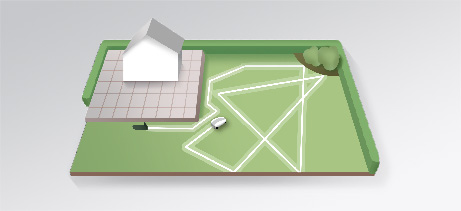
\includegraphics[scale=0.8]{figures/noLogiCut.jpg} 
\label{fig:randomcut}
\caption{Random cut system [source:Bosch]} 
\end{figure}

\noindent
When the battery is nearly discharged, the mower will follow the guard wire back to the base station for recharging.\\\\
\noindent
Parallel line mowers use a more intelligent control algorithm to optimize the mowing. After an initial learning run, following the guard wire around the lawn to be mowed, it will map the lawn, and cut in parallel lines, see \figref{fig:logicut}. The advantage of this strategy efficiency, as the lawn mower will not run over the same spots more than once. According to Bosch, a given lawn can be mowed up to 30\% faster with their Logicut system.
%% TODO: Insert source
 

\begin{figure}[H]
\centering
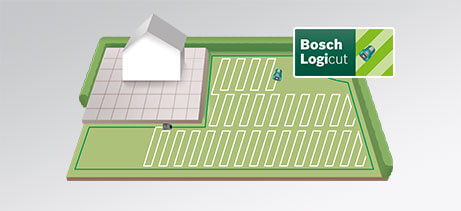
\includegraphics[scale=0.8]{figures/logicut.jpg} 
\label{fig:logicut}
\caption{Bosch Logicut system [source:Bosch]} 
\end{figure}

\noindent
Common for both systems is the guard wire, which has to be placed around the lawn and anywhere the lawn mower is not allowed to go, like flower beds, swimming pools, etc. \\\\
\noindent
This brings us to the problem with existing products.

\section{Problems with existing robotic lawn mowers}
All commercially available robotic lawn mowers requires a guard wire placed around the lawn. This can either be placed at the surface, and be held in place by pegs, or dug down below the surface. The guard wire must be routed around flower beds, etc. as well, see \figref{fig:robomow}

 
\begin{figure}[H]
\centering
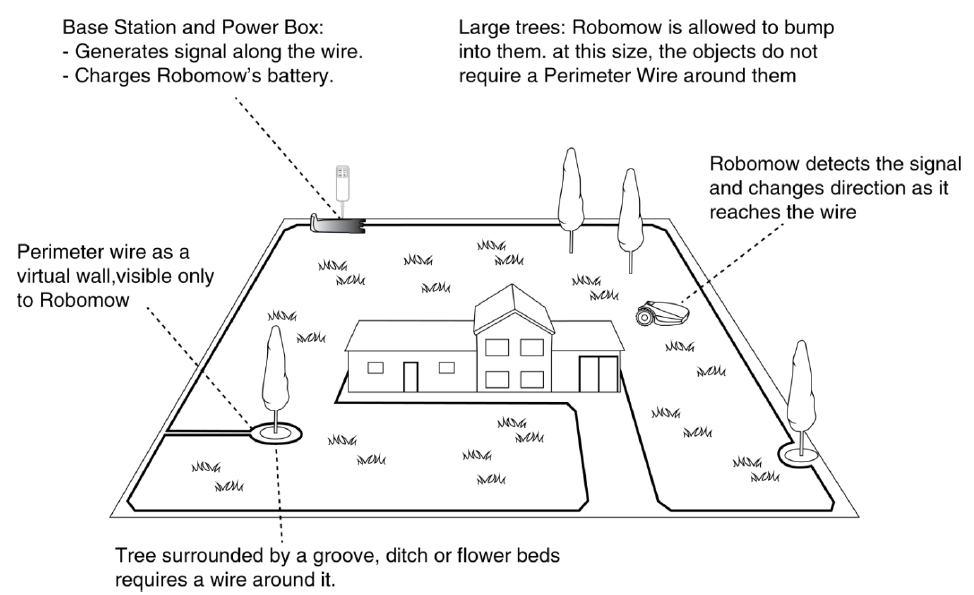
\includegraphics[scale=0.6]{figures/robomow.png} 
\label{fig:robomow}
\caption{Guard wire installation [source:Robomow]} 
\end{figure}
\noindent

The use of the guard wire for guiding the mower back to the charging station presents another potential problem: in a garden with many restricted areas, the guard wire could get very long. This could therefore make the journey home long, compared to a more direct route. This again uses more battery power, that instead could have been used for actually mowing the lawn.\\\\
\noindent
This will be the motivation for the project: to avoid the work routing a wire around the garden, and as a bonus get more work done on a battery charge, by not wasting power following the wire home.\\\\
\noindent
Then, the question is: What other solutions could be use to get the lawn mower to go where it has to go? \\
One first step could be to keep track of where it is in real-time.
%-- Section : GoT introductory presentation --%
\section{The Games on Track (GoT) system}
We were provided with the \emph{Games on Track GT-Position} system as a start to be able to determine the lawn mower's position in space. 
% Add reference to GoT description

\begin{figure}[H]
\centering
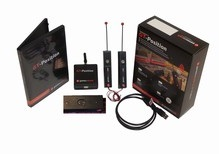
\includegraphics[scale=1.1]{figures/gotSystem.jpg} 
\label{fig:gotsystem}
\caption{Games on Track GT-Position package [source:Games\ on\ Track]} 
\end{figure}
\noindent

\noindent
It is composed of four different parts both hardware and software :
%% TODO : Add reference to http://www.gamesontrack.co.uk/pages/webside.asp?articleGuid=64556
\begin{itemize}
	\item A tracked module, which emits ultra-sound waves. It should be placed on the lawn mower itself while taking care, that the emitting cell is not obstructed by anything.
	\item Beacons or receivers, placed around the area the lawn mower will move in. Depending on the terrain, anywhere from 2 \todo{--Resolved-- is two enough? Answer: It is according to the GoT site (see reference in LaTeX comments)} to more than 20 of these can be used: the more is placed, the more accuracy can be obtained to fight against any ambient noise.
	\item The central system, which calculates the distance of the tracked module to each beacon, and transmits it to the computer via USB in regular intervals.
	\item The GoT software aggregates the received positions throughout time, and can be used to draw a map of the terrain (the lawn), and to determine the absolute position of the tracked module.
\end{itemize}

GoT was originally designed for train modelling, but it is easily adaptable for any use of position tracking and seems a good choice, at first, for our autonomous lawn mower.
But, why not use a satellite based positioning system ?

%-- Section : Satellite vs GoT --%
\section{Satellite based positioning systems vs GoT}
\todo{Wrong reasons for GPS vs GoT, elaborated below}
The reasons why satellite positioning system won't be used in our project are mainly related to accuracy over price ratios and to energy consumption.\todo{--To be reviewed again-- GPS uses very little power -> depending on the accuracy needed...}

\noindent
Indeed, these kinds of system like GPS or GLONASS would require a dedicated chip to put on the final system. The problem then would be the lack of precision. Although, there are some cheap standard GPS chips (around USD 10), these only reach around 1 meter of precision in the most ideal situations. % ref : www.gps.gov
On the other hand, the best GPS chips can achieve precisions up to a few millimeters when combined with different augmentation systems (algortihms for instance), but they end up being highly expensive (usually thousands of dollars). They are not generally intended for public use.
\todo{--To be reviewed again-- Only applies to cheap solutions, differential GPS can go to mm level, but is extremely expensive. This is what we are trying to replace with GoT, as it is a lot cheaper than diff-GPS} \\\\
%% TODO : Add reference to "A Review of GLONASS" Miller, 2000 & http://www.gps.gov/systems/gps/performance/accuracy/ 
\noindent
Moreover, if we add up the slow bit rates satellites can achieve, the signal amplifiers on the receiver, plus all the position calculations and possible augmentation systems, the total energy consumption would quickly rise,\todo{--To be reviewed again-- nope, it's just a radio receiver, uses almost no power} thus reducing the lawn mower autonomy, which is not desirable.\\
Indeed, the design of a product has no real value if no one is interested in using it. This is why choices made during this project have to be made in accordance with the final user's expectations.\\\\
\section{Potential consumer expectations}
Usually, we can think of a few priorities consumers will have when buying a product, whatever it is, and some more specific to technical products.\\
\noindent
Here for instance, the autonomy of the vehicle (both in energy and for the navigation), and the overall cost should be considered. The GoT system itself has a cost (USD 606.00 for a basic package) beyond anything a normal customer would probably pay for a lawn mower. But despite that, it appears, at first, to be a good solution for us in terms of accuracy and energy consumption compared to GPS-like systems which are even more expensive for the same accuracy. \todo{--Resolved-- insert price approximation here - not so true actually} \\\\
\noindent
These are the types of preliminary considerations that will influence this design process for an autonomous lawn mower.
\section{Robotic Lawn Mowers}\label{roboMowers}
Several manufacturers of electrical gardening machines have started selling robotic lawn mowers in the recent years. In general they use one of these two strategies when cutting the lawn \todo{Source}:
%
\begin{itemize}
	\item Random direction mowers.
	\item Parallel line mowers.
\end{itemize}
%
Mowers utilizing the random direction strategy will drive in a straight line until a guard wire or an obstacle is detected. They will then turn in a random direction, and continue. See \figref{fig:randomcut}.

\begin{figure}[H]
\centering
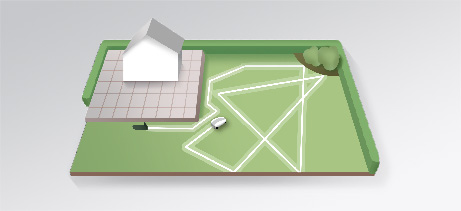
\includegraphics[scale=0.8]{figures/noLogiCut.jpg}
\caption{Random cut system \cite{Bosch}} 
\label{fig:randomcut}
\end{figure}
\noindent
When the battery is nearly discharged, the mower will follow the guard wire back to the base station to recharge.
%
Parallel line mowers utilize another control algorithm for mowing. After an initial learning run, following the guard wire around the lawn to be mowed, it will map the lawn, and cut in parallel lines, see \figref{fig:logicut}. The advantage of this strategy, is that the lawn mower will not run over the same spots more than once. According to Bosch, a given lawn can be mowed up to 30\% faster with their Logicut system \cite{Bosch}.

\begin{figure}[H]
\centering
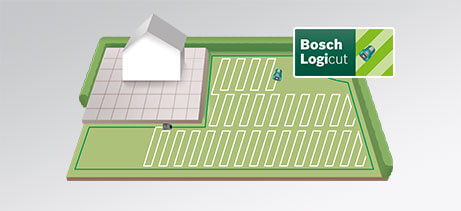
\includegraphics[scale=0.8]{figures/logicut.jpg} 
\caption{Bosch Logicut system \cite{Bosch}}
\label{fig:logicut}
\end{figure}
\noindent

Common for both systems is the guard wire, which has to be placed around the lawn and anywhere the lawn mower is not allowed to go, like flower beds, swimming pools, etc.
\subsection{Existing Problems}
Some commercially available robotic lawn mowers require a guard wire placed around the lawn. It can either be installed at the surface, and be held in place by pegs, or dug down below the surface\todo{source?}. The guard wire must be routed around flower beds, bushes etc. as well, see \figref{fig:robomow}.\\\\
%
The use of the guard wire for guiding the mower back to the charging station presents another potential problem: in a garden with many restricted areas, the guard wire could get very long. Therefore the journey home could be longer, compared to a more direct route. This again uses more battery power, that could have been used for actually mowing the lawn instead.\\\\
%
This will be the motivation for the project: to avoid the work routing a wire around the garden, and as a bonus get more work done on a battery charge, by not wasting power following the wire home.\\\\

\begin{figure}[H]
\centering
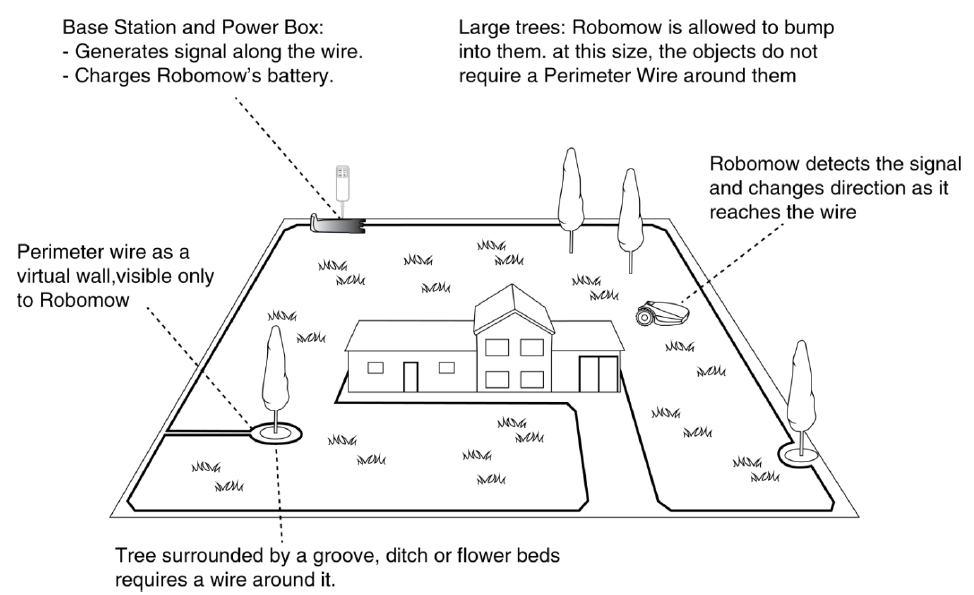
\includegraphics[scale=0.6]{figures/robomow.png} 
\caption{Guard wire installation [source:Robomow]}
\label{fig:robomow} 
\end{figure}
\noindent

Then, the next question is: what other solutions could be used to get the lawn mower to go where it has to go?
A solution of keeping track of the lawn mower's position in real-time is examined.
%-- Section : GoT introductory presentation --%
\section{The Games on Track System}
One available system is the \emph{Games on Track GT-Position} system, referred to as GoT. The GoT would be able to determine the lawn mower's position in space, see \secref{sec:Vehicledescription}. It is composed of three different parts both hardware and software \cite{GoTWebsitePos}:

\begin{itemize}
	\item A tracked module, which emits ultra-sound and radio waves. It should be placed on the lawn mower itself.
	\item Towers which are tracking the tracked module placed on the vehicle are needed. These should be located around the area where the lawn mower will move. There should be at least 3 towers, depending on the terrain, and can be up to more than 20. The more towers, the more accuracy can be obtained to cancel out any ambient noise, and more space can be monitored.
	\item The master, connected to a computer, receives data from the towers and transmits it to computer through a USB in regular intervals. The distance of the tracked module is then calculated by the computer.
\end{itemize}

\begin{figure}[H]
\centering
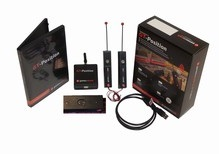
\includegraphics[scale=1.1]{figures/gotSystem.jpg} 
\caption{Games on Track GT-Position package [source:Games\ on\ Track]} 
\label{fig:GoTsystem}
\end{figure}
\noindent
%
The GoT software aggregates the received positions through time, and can be used to draw a map of the lawn, and to determine the absolute position of the tracked module.

GoT was originally designed for train modelling, but it is easily adaptable for any use of position tracking. In the following segment satellite based positioning systems are compared to the discussed GoT system.
%-- Section : Satellite vs GoT --%
\section{Satellite based positioning systems vs GoT}
\todo{Wrong reasons for GPS vs GoT, elaborated below}
The reasons why satellite positioning system won't be used in our project are mainly related to accuracy-over-price ratios and to energy consumption.\todo{--To be reviewed again-- GPS uses very little power -> depending on the accuracy needed...}\\\\
Indeed, these kinds of system like GPS or GLONASS would require a dedicated chip to put on the final system. The problem then would be the lack of precision. Although, there are some cheap standard GPS chips (around USD 10), these only reach around 1 meter of precision in the most ideal situations \cite{GPSUSWebsiteAccuracy,Miller}. \\
On the other hand, the best GPS chips can achieve precisions up to a few millimeters \cite{GPSUSWebsiteAccuracy} when combined with different augmentation systems (algortihms for instance), but they end up being highly expensive (usually thousands of dollars). They are not generally intended for public use.
\todo{--To be reviewed again-- Only applies to cheap solutions, differential GPS can go to mm level, but is extremely expensive. This is what we are trying to replace with GoT, as it is a lot cheaper than diff-GPS} \\\\
%
Moreover, if we add up the slow bit rates satellites can achieve, the signal amplifiers on the receiver, plus all the position calculations and potential augmentation systems, the total energy consumption would quickly rise, \todo{--To be reviewed again-- nope, it's just a radio receiver, uses almost no power} thus reducing the lawn mower autonomy, which is not desirable.\\\\
%
Indeed, the design of a product has no real value if no one is interested in using it. This is why choices made during this project have to be made in accordance with the final user's expectations.
\section{Consumer Expectations}
Usually, consumers have a few priorities when buying a product, whatever it is, and some more specific for technical products.\\
Here for instance, the autonomy of the vehicle (both in energy and for the navigation), and the overall cost should be considered. The GoT system itself has a cost (around \$ $600.00$ for the most basic package) beyond anything a normal customer would probably pay for a lawn mower. But despite that, it appears, at first, to be a good solution for a basic autonomous lawn mower in terms of accuracy and energy consumption compared to systems like GPS which are even more expensive for the same level of accuracy. \\\\
These are the types of preliminary considerations that will influence this design process for an autonomous lawn mower.

%---------- Chapter 2 ----------------------------------------
\chapter{Design Considerations}
\vspace{-5 mm}
In this chapter the system is designed with a top-down approach, which means an overview of the system is formulated first. Thereafter the system will be broken down into smaller segments. First a use-case model of the system, where the functionalities and the coherent actors is described, in order to give an overview of what the system must be able to do. Thereafter, constraints set by time limitations as well as a focus on the main scope of the project, in regards to the prototype, are considered.
\vspace{-4 mm}
\section{Use-case Design} \label{sec:UseCase}
To give an overview of what the system should be able to do, a use case with coherent actors is utilized. The use case diagram, see \figref{fig:usecase}, will describe the main functionalities in the use case as well as describing the actors, the external sensors and systems, affecting the system.

%The use-case diagram is made, where the micro controller is the system that will be analysed, because, it will be the master in this system

\vspace{-3 mm}
 \begin{figure}[H]
	\centering
	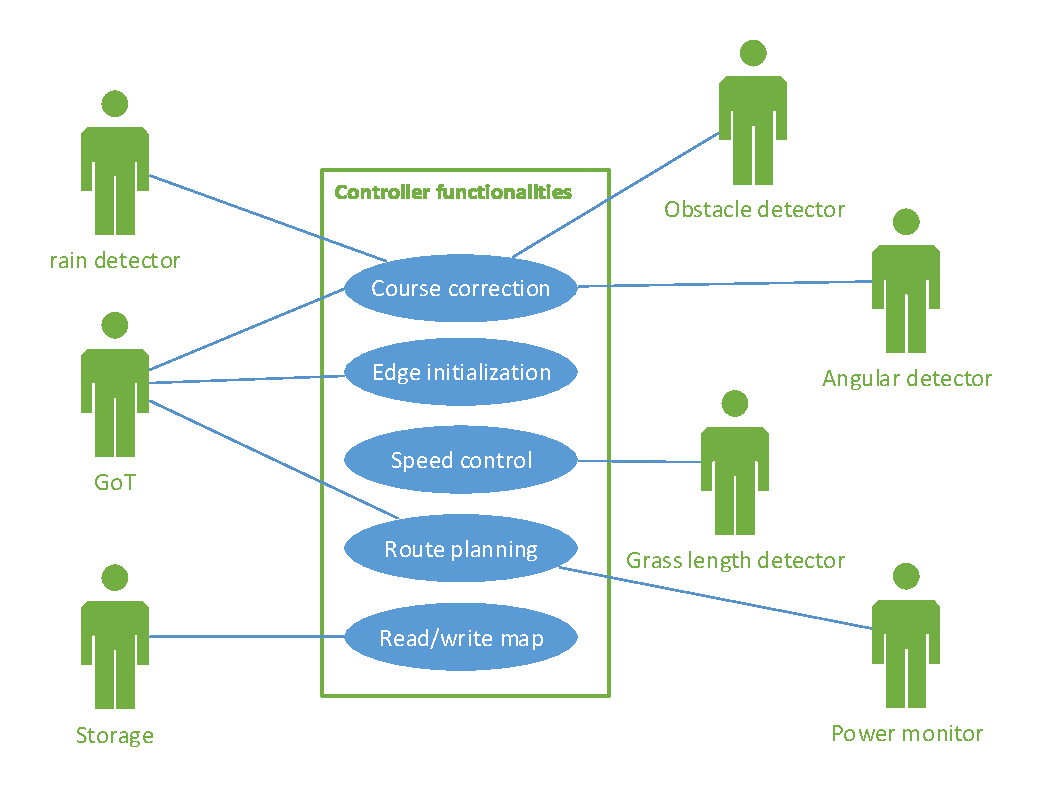
\includegraphics[scale=0.8]{figures/P5UseCase.pdf}
	\caption{Use-Case Diagram}
	\label{fig:usecase}
\end{figure}

\noindent
\newpage

The system, inside the controller, have 6 main functionalities and is affected by 9 different actors.

\subsection{Main Functionalities}

Functionalities are the functions that the system can do. Each Functionality can have more than one function in the system. The functionalities get input from actors and can be in association with other functionalities. 

\textbf{Edge Initialization}:
The \textit{Edge Initialization} gets input from the \textit{GoT} system and is associated with the \textit{Read/Write Map} functionality. The purpose of this function, is to calibrate the system to a new lawn, by mapping the edge of the lawn. The edges which is mapped should include the area in which the vehicle should stay inside and the areas which it should avoid, e.g. trees, bushes and so on. This is done, by first manually moving the \textit{GoT} system's transmitter along periphery of the lawn and thereafter along the edges of obstacle placed on the lawn. This could be performed by the use of a button which could make the system record edges if pressed. The information about the edges, an edge map is created and saved through the \textit{Read/Write Map} function.

\textbf{Route Planning}:
The \textit{Route Planning} gets input from the \textit{Power Monitor} and is associated with the \textit{Read/Write Map} functionality. The purpose of this function, is to plan the route for the lawn mower. The route is created by knowing where the lawn mower is located and the map of edges of the lawn, which is located in \textit{Storage}. The map is loaded from the \textit{Storage} with the \textit{Read/Write Map} function. Furthermore it acquires the voltage level of the battery from the \textit{Power Monitor}, to ensure it will return to base before it runs out of battery.

\textbf{Read/Write Map}:
The \textit{Read/Write Map} gets input from the \textit{Storage} and is associated with the \textit{Route Planning}, \textit{Course Correction} and the \textit{Edge Initialization} functionalities. This functionality is the link between functionalities and \textit{Storage}. The edge map retrieved from \textit{Edge Initialization} and through use of the \textit{Read/Write Map} function, is stored in the \textit{Storage}. In \textit{Storage}, the route which calculated by the \textit{Route Planning} is also located. The \textit{Course Correction} functionality also needs access to the \textit{Storage} to be able get the calculated route.

\textbf{Course Correction}:
The \textit{Course Correction} gets input from the \textit{GoT} system, the \textit{Humidity Detector}, the \textit{Obstacle Detector} and the \textit{Angular Detector} and is associated with the \textit{Read/Write Map} and the \textit{Speed Control} functionalities. This function gets both an angle and the humidity in the air as input, furthermore it gets an input if it encounters an obstacle blocking its path. \textit{Course Correction} takes all these parameters into consideration when navigating from its last registered position, retrieved from the \textit{GoT} system, to the next destination on the calculate route retrieved from the \textit{Storage} trough \textit{Read/Write Map}. The \textit{Course Correction} is the main function behind the regulation of the vehicle's angular movement. The  \textit{Course Correction} decides the velocity, according to the calculated route, and passes the decided velocity to the \textit{Speed Control}.

\textbf{Speed Control}:
The \textit{Speed Control} gets input from  the \textit{Grass Length Detector} and the \textit{Speed Measurement} and is associated with \textit{Course Correction}. The function's purpose, is to make sure that the lawn mower adapts the speed depending on the grass length and if the \textit{Course Correction} ask for a different velocity, e.g. if the vehicle is going into a curve.

\textbf{Blade Control}:
The \textit{Blade Control} gets input from the \textit{Blade Monitor}. The function's purpose, is keeping the blade rotational speed the same, to make an even cut grass. With the input from the \textit{Blade Monitor}, the \textit{Blade Control} can regulate the velocity of the blade.

\subsection{Actors}
A actor is a component, that influence the system by giving inputs to the functionalities and/or receiving outputs from them.

\textbf{GoT}:
The \textit{GoT} system is connected to the \textit{Course Correction}, the \textit{Route Planning} and the \textit{Edge Initialization} functionalities. This system is used to retrieve the GoT transmitter's, placed on the vehicle, location on the lawn. The GoT system is explained in \appref{GoTDescription}.

\textbf{Storage}:
The \textit{Storage} is connected to the \textit{Read/Write Map} functionality. It uses a non-volatile storage to store the information about the edge map and route, which is made in the \textit{Edge Initialization} and \textit{Route Planning} functionalities. This will make the \textit{Storage} able to keep the data even if the system is turned off.

\textbf{Humidity Detector}:
The \textit{Humidity Detector} is connected to the functionality \textit{Course Correction}. This is a sensor that measures the humidity in the air. The system uses the information about the ambient humidity level to see, whether the grass is too wet for mowing the lawn, since wet grass can not be cut evenly. 

\textbf{Obstacle Detector}:
The \textit{Obstacle Detector} is connected to the \textit{Course Correction} functionality. This sensor detects, if there are any objects, which blocks the lawn mower's route. This sensor makes sure, that the lawn mower registers objects, like a human or a dog, which could interfere with the lawn mower's route.

\textbf{Angular Detector}:
The \textit{Angular Detector} is connected to the \textit{Course Correction} functionality. This sensor measures the angular position and movement of the lawn mower, whether it is intentional movement or if the lawn mower slips.

\textbf{Grass Length Detector}:
The \textit{Grass Length Detector} is connected to the \textit{Speed Control} functionality. This sensor measure the  grass length, which affects the velocity, at which the lawn mower should drive. If the grass is long, the lawn mower has to drive slower, to make sure that it cuts the grass evenly. 

\textbf{Power Monitor}:
The \textit{Power Monitor} is connected to the \textit{Route Planning} functionality. This sensor measures how much power is left in the battery. This is needed, so that the lawn mower can drive back to its charging station, before the battery is too low, to not destroy the battery.

\textbf{Blade Monitor}:
The \textit{Blade Monitor} is connected to the \textit{Blade Control} functionality. This sensor measures the rotational speed of the blade and send the information back to the \textit{Blade Control}

\textbf{Speed Measurement}:
The \textit{Speed Measurement} is connected to the \textit{Speed Control} functionality. The sensor measure the speed of the lawn mower.
\section{The Vehicle}

\subsection{The vehicle in general}


\subsection{Hall Sensor}
There are two hall sensors implemented on the vehicle, one by each drive gear, illustrated in \figref{vehicleDescriptionDriveTrain}. Four magnets are placed on each drive gear, with a quarter turn between each. The Hall sensor is illustrated in \figref{HallSensor}.

\begin{figure}[H]
	\centering
	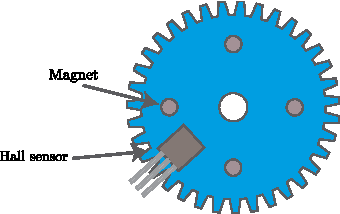
\includegraphics[scale=1.2]{figures/hallSensorDrawing.pdf}
	\caption{Illustration of the drive gear, with the magnets and the Hall sensor. The Hall sensor is placed stationary beside the rotating gear \cite{KHSoerensen}.}
	\label{HallSensor}
\end{figure}\vspace{-5mm}
%
A Hall sensor is affected by magnetic fields. When the field is significantly larger than the ambient fields a pulse is generated. This gives a voltage output each time one of the magnets is in front of the Hall sensor. Therefore each time the drive gear makes a quarter of a turn a voltage signal is generated.

%As the distance between each magnet is not exactly a quarter of a turn, the calculations of the pulses received from the Hall sensor, is processed for each magnet independently.
%By measuring the time between five outputs, as the first and the fifth output is from the same magnet, the time of a whole rotation of the gear can be found. By knowing the distance the vehicle travels for a full rotation of the gear, the speed can be calculated.
%
%When the vehicle is starting to move, the speed of the first turn of the gear can not be calculated. This is because two signal from the same magnet are needed before the speed can be calculated. So the first four output from the hall sensor will be saved and at the fifth output, after a whole turn, the speed related to the first magnet will be calculated.\\
%
%The hall sensors are used to measure the speed of the two belts, which will run at different speeds when the vehicle is turning. Now that the components linked to the velocity  are described, the steering material will be analysed.

\subsection{Servo}
On the vehicle there is a servo, which is a S3003 by Futaba.
The servo is used for the steering of the vehicle. The servo controls the steering through breaking one of the belts and transfer that power over to the other belt.


The Servo is controlled by a PWM signal. The PWM signal recieved is converted into an angle by the servo to control the steering of the belts, as seen on \figref{timeVSangle}. An angle of 90° is the normal position for going straight, while 0° and 180° are the limits for turning, where one of the belts is not moving. 

A mechanical arm is mounted on the servo and connected to the brakes of the tracks. When the servo rotates one way, it triggers the brakes more on one side and less on the other side, according to the value of the angle sent, through the PWM signal. This way, one of the belt will drive slower and the other belt drive faster, which will make the vehicle turn, without decreasing the motor power.

The servo reacts lineary to the PWM signal and the cycle of the signal is 30 milliseconds. To get the servo to be in neutral position, the servo needs a PWM signal of 4.83 \% (a period of 1450 microseconds). For 180°, it is 8.33 \% (a period of 2500 microseconds) and 1.67 \% (a period of 500 microseconds) for 0°. \\

%source http://www.societyofrobots.com/actuators_servos.shtml\\

\begin{figure}[H]
	\centering
	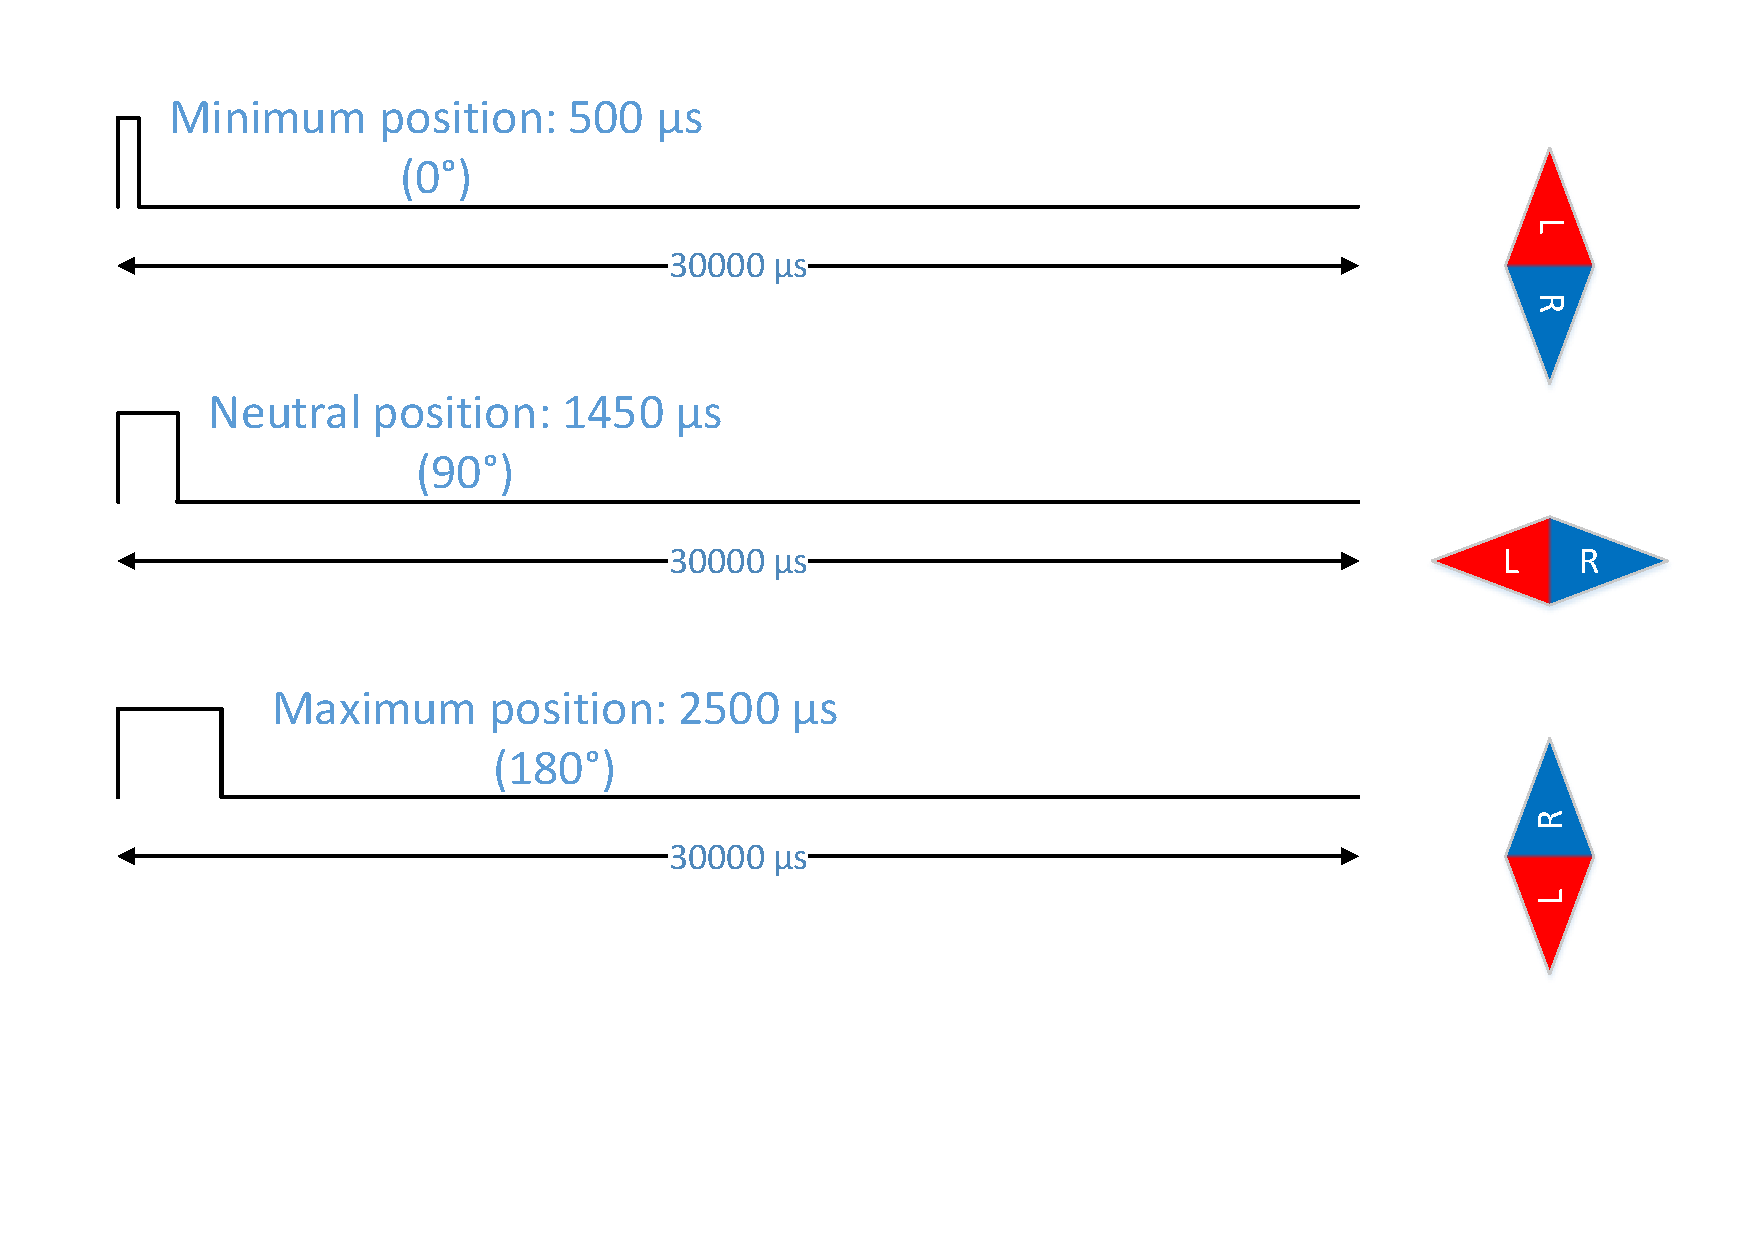
\includegraphics[scale=0.6]{figures/TimeVSangle.pdf}
	\caption{Convertion from time to angle by the servo}
	\label{timeVSangle}
\end{figure}


\subsection{Differential gears} \label{sec:Differentialgears}

When the servomotor is braking, it triggers the differential gears to make the vehicle turn.\\
Differential gears are used to reduce slipping between opposite wheels when a car is turning. The system can not avoid slipping under the tracks because they are too long, they will rotate at least around the center of the track. However, using differential gears will help control the course of the vehicle by transfering the power of the braking track to the other track.\\

As seen on \figref{diffGearLight}, the power is transmitted from the pinion gear (not represented on this picture) to the spider gear (here in green) fixed on the ring gear (here in blue). Only the spider gear is connected to the side gears(here in pink and yellow), fixed to the wheels.\\

\begin{figure}[H]
	\centering
	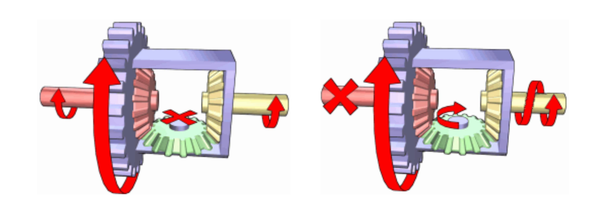
\includegraphics[scale=0.7]{figures/diffGearLight}
	\caption{Transfer of the power to the side gear when the spider gear is blocked versus when it spins \cite{MechanicalEngineering}}
	\label{diffGearLight}
\end{figure}

When the ring gear is turning but the spider gear does not spin, both side gears turn the same speed. But if one side gear is blocked, the spider gear will spin,  and the other side gear will turn faster.\\

There are usually two spider gears (here in red) for more reliability and solidity, and the ring gear (here in blue) is set in motion by the pinion gear (here in brown in front) as seen on \figref{diffGearFull}.\\

\begin{figure}[H]
	\centering
	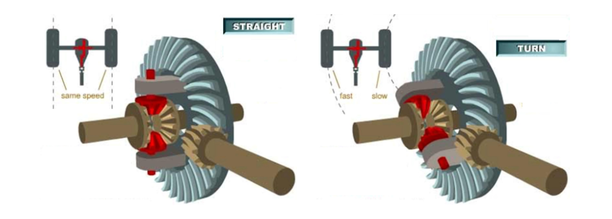
\includegraphics[scale=0.7]{figures/diffGearFull}
	\caption{Description of the differential system going straight vs turning \cite{MechanicalEngineering}}
	\label{diffGearFull}
\end{figure}

This is the element the servo is using when braking one track, allowing the other track to turn still.\\\\



The description of the vehicle allows then to consider a prototype of the functionnalities needed in this project.



\section{Prototype Constraints}\label{sec:PrototypeConstraints}
Before the prototype can be established, some considerations have to be made in respect to time limitations and the main scope of this semester. The aim of the project is to create a functional automated proof of concept lawn mower. The following section provides argumentation for eliminated functionalities from the use case \secref{sec:UseCase}.

\subsection{Grass Length Detection}
Detection of the grass length to control the velocity of the lawn mower thus ensuring an evenly cut lawn, is a submodule which can be added at any time. Since it is not fatal for a working system and might even be unnecessary depending on time between each mowing of the lawn, it is decided to exclude this functionality from the initial design.

\subsection{Humidity Sensor}
As the lawn mower is supposed to work outside, it is important to consider that the grass could be humid. Since it is difficult to cut wet grass, a humidity sensor could be used to warn the system of the humidity, thus the system could go back to the charging station. This submodule is not fatal for a functional prototype, so this type of sensor will not be included in the design.

\subsection{Obstacle Avoidance}
The lawn movers path might not always be clear, e.g. garden tools, tables or moving objects could be in the way. The vehicle should be aware of what is in front of it at any time, to correct its path and be able to get around the obstacle if necessary. To avoid this the sensor could be a pushing button to detect a solid object or an ultrasound detector if the object is fragile.
As the aim of the project is to control the path of the vehicle by using angular positioning sensors, a proximity sensor will not be included. Static objects could be registered on the map to avoid these issues.

Furthermore the edge mapping functionality will not be included in the project which instead will focus on a map predefined in the test room.

%\subsection{Power Monitoring}
%Power monitoring could be implemented by measuring the voltage across the batteries, to ensure that the lawn mower is not running out of power, and to ensure the vehicles calculated route passes the charging station before the power runs too low.
%This and the charging station will not be in the prototype, since it is beyond the scope of the project this semester and is not crucial for a working prototype.

\subsection{Blade Control \& Blade Monitor}
To get the blade to cut the grass evenly over the whole lawn, the blade control and monitor is needed to keep the blade at the same velocity.
The blade, and therefore the blade control and monitor, will not be in the prototype. This is because, the focus of the project is on the movement of the vehicle and the blade does not contribute to this and is therefore not relevant.

\subsection{Route Planning}
Route planning is a way to optimizing the lawn mowers time on the lawn, instead of the classic solution with a random cut system, describe in \secref{roboMowers}. The prototype will not have a algorithm calculating a route from the vehicle's position, the battery time and information received from the edge map. The route in which to follow is a predefined route made to illustrate and test the essential part of the prototype.

\subsection{Testing}
The testing will take place in Aalborg University Vicon Room, where the GoT system is installed, see \secref{GoTDescription}, is installed and calibrated with the appurtenant transmitter, which is mounted on the tracked vehicle during test.

A description of the system and arguments for eliminating functionalities from the initial design has been presented in the preceding segment. The prototype can now be established in regards to the equipment available and remaining functionalities.

\section{Prototype, Interfaces and Submodules} \label{Finalprototype}
%The overall functionalities for the project have been limited, due to time limitations and to focus on the scope of the project. In this project a prototype will therefore be made to show the main functionalities necessary to make an automated vehicle containing principles for lawn mowing.
%In short, the final prototype includes a regulator, which will make it possible to follow a path from A to B. It is able to continue if the wireless connection is lost between the prototype and the GoT system for some duration. Furthermore it is able to plan a route within a given area and store these calculated data points locally, on the vehicle. The rough outline of the design is shown in \figref{fig:systemOverview1} to give an idea of the final prototype setup.

%\begin{figure}[H]
%	\centering
%	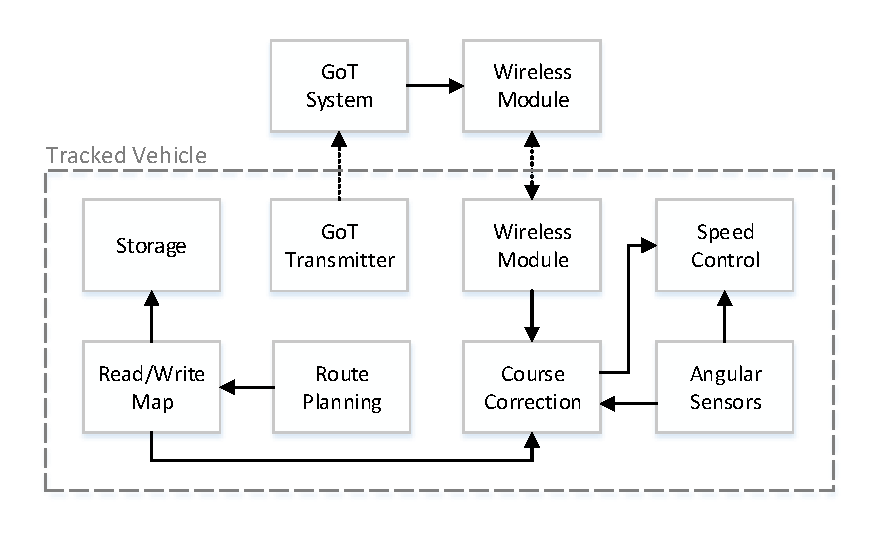
\includegraphics[scale=.9]{figures/systemOverview1}
%	\caption{Overview of the system prototype}
%	\label{fig:systemOverview1}
%\end{figure}

%The GoT system provides the vehicle with coordinates, which is utilized in course correction in combination with the map supplied from storage, to follow the route. In course correction lies also control between coordinates given by the GoT system and the storage, this is regulated through use of angular position and movement supplied by the angular sensors. The speed control gets an input from the course correction, the speed given is then held through regulation again using input from angular sensors, in this case specifically acceleration.


%Previously the rough prototype design is presented. To provide a more broad overview of the system, an exploded view of functionalities, their submodules and interfaces is presented in \figref{fig:systemOverview2}.

The overall functionalities for the project have been constrained from the Use-Case \secref{sec:UseCase}, due to time limitations and to focus on the main scope of the semester. A prototype is therefore made to illustrate the main functionalities necessary to make an automated vehicle, containing principles for lawn mowing.

The final prototype includes a regulator, which will make it possible to follow a path from A to B. It is able to continue if the wireless connection is lost between the prototype and the GoT system for some duration. The outline of the design is shown in \figref{fig:systemOverview2} to give an idea of the final prototype setup. In this section, the different functional blocks are put forth along with the interfaces describing the interaction between them.

\begin{figure}[H]
	\centering
	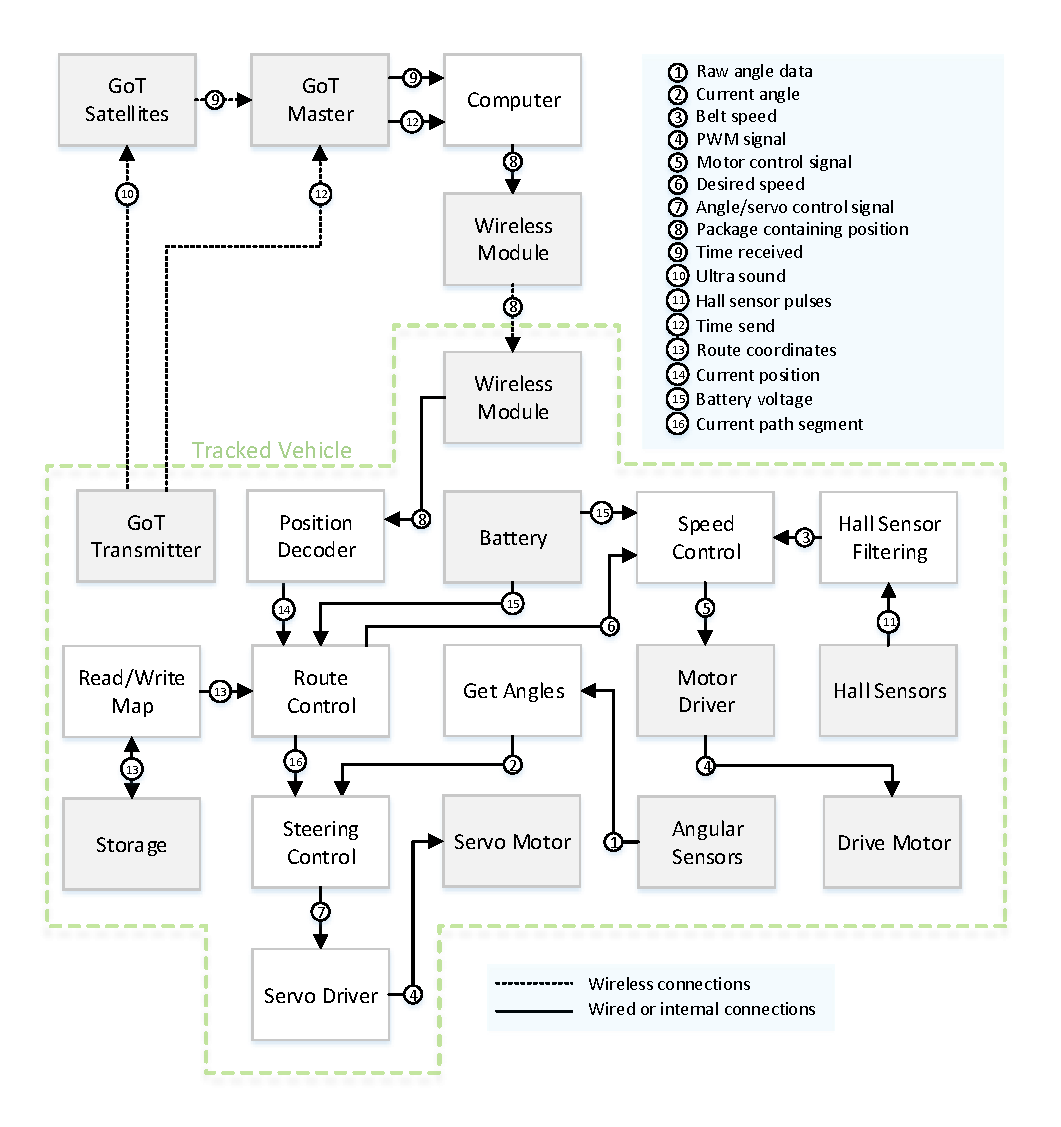
\includegraphics[scale=.9]{figures/systemOverview2}
	\caption{Overview of the software and electronic parts of the system prototype, where the gray modules are hardware and the white are software.}
	\label{fig:systemOverview2}
\end{figure}

\subsection{Modules}
In the following all the modules from the system prototype which needs further explanation are described to obtain a basic understanding of the prototype.

%\subsubsection{GoT System}
%%The GoT satellites is placed in the area in which the vehicle needs to operate. These satellites receives information from the vehicle. The time which the vehicles transmitter sends out bursts is received by the GoT master. Furthermore the time which the satellites receives the information send from the vehicles transmitter is transmitted to the GoT master. The GoT master then relays the information received from the vehicle directly to the 
%
%The \textit{GoT Transmitter} placed on the vehicle transmits a signal containing the time at which it send the ultra sound signal to the \textit{GoT Satellites} to the \textit{GoT Master}. The satellites transmit the signal recieved to the master as soon as they recieve it. The master then relays those informations to the \textit{GoT on Computer} that will calculate the position of the car.

\textbf{Computer and Position Decoder:}
The computer handles the calculation of the current position of the vehicle \secref{sec:Vehicledescription}. If a packet is disturbed or sent incorrectly it should be possible to detect it, so invalid data is not used by the prototype. It may occur that the coordinates which are sent from the GoT system is out of sensible range, e.g the coordinate transmitted jumps from one location to a location which is unrealistic for the vehicle to reach in the amount of time between received coordinates. In this event the out of range coordinate should also be disregarded. The computer must compile a package containing the coordinates. The position decoder must be able to decode the transmitted package.

%\textbf{Route Planning:}
%This module receives the vehicle's position from the GoT and the next destination on the path, which is located in the storage. This information constitutes a desired path segment on which the vehicle must stay. The desired path segment is passed along to steering control.
%The route planning also monitors the battery voltage, and plans a route back to base when the battery starts running low. This is of course to ensure that the vehicle does not get stuck on the lawn, but also to protect the battery, which might get damaged from excessive discharge.

\textbf{Steering Control:}
This module makes sure that the vehicle stays on its path, which it receives from storage. To achieve this the steering control also receives the current path segment of the vehicle, which it uses to calculate a desired angle. The desired angle is used in comparison with the current angle in the steering control to regulate course of the vehicle.

\textbf{Read/Write Map:}
This module handles the writing of coordinates to the non-volatile storage device, as well as the reading of next desired destination from the stored route.

\textbf{Speed Control:}
This module retrieves the speed of the vehicle from the Hall Sensor Filtering module. This is used, through control, to obtain a steady speed. Furthermore it handles any request of change in speed delivered by the course correction.

%\subsubsection{Edge Map}
%The first time the user will initialise the lawn mower, an \textit{Edge Map} will be created thanks to the GoT system. This edge map will determine the areas that the car is allowed to go or not, in regards of specifications or objects on the lawn.  

%\subsubsection{Route Planning}
%The Route Planning module calculates a route from the points gathered from the Edge Map. The route will be in straight lanes, as in the Bosch Logicut system \secref{roboMowers}, to guarantee that the whole lawn is cut.

%\subsubsection{Angular Sensors}
%The angular position is measured thanks to the \textit{Angular Sensors}, that will send data to the submodule \textit{Get Angle}, in charge to send the angle to the Speed Control and to the Course Correction submodule.

\subsection{Interfaces}
%- To Tom and Rasmus \newline
%In the subsection an explanation of the different interfaces between the modules is made. We have thought about making it like a high layer interface, where we only explain what we need the different modules to give each other. Like one module needs to get the map edge, i.e. coordinates, but since it is this early in the report and it would be more overview by writing map edge rather than coordinates. But as you can see in \figref{fig:systemOverview2} the layers of information are different, one is raw angle data and another time send. Is this okay or should we change something else?
%\indent
%The interfaces of the system is very important when designing each of the adjacent submodules. The existing interfaces as well as the ones presumed are also important in the process of analyzing the system capabilities width focus on requirements of the prototype. Width that in mind follows a brief review of the interfaces between each submodule.
In this section a high layer interface between the modules will be presented. This provides information for designing each of the adjacent submodules individually.

\textbf{Package Containing Position (8):}
The data communicated from the GoT system to the Position Decoder on the vehicle contains the last recorded position of the vehicle. This position is presented in the form of an x- and a y-coordinate, which must be included in the data package. Additionally each package must contain decode information for the receiver, including how to separate each package along with error handling.

\textbf{Angle/Servo Control Signal (7) and PWM Signal (4):}
Course correction will ask the vehicle to turn or make small adjustments to the angle. This angle adjustment is realized through the servomotor which brakes on either belt appropriate to the required angle. For the servo to understand the angle, the servo driver must translate it into a PWM signal, which makes the servo turn to a specific position for each pulse width.

\textbf{Route Coordinates (13), Current Position(14) and Battery Voltage (15):}
Route coordinates are extracted from the storage and paired with the current position given by the GoT system. This coordinate pair yields a path segment for the vehicle to follow, which is forwarded to steering control.

\textbf{Raw Angle Data (1), Current Angle (2) and Current Path Segment (16):}
The raw angle data is translated to a current angle of the vehicle. Current angle is then used to calculate the desired angle using the path segment given by route planning.

\textbf{Desired Speed (6), Motor Control Signal (5) and PWM Signal (4):}
Desired speed is regulated by the route control because the route planner knows when the vehicle must turn, in which case the speed should be lowered, if desired. The speed controller makes sure that the vehicle stays at this speed, until told otherwise, by regulation of the motor control signal. This signal is then translated, by the motor driver, to a PWM signal for the motor.

\textbf{Hall Sensor Pulses (11) and Belt Speed (3):}
To determine the speed of the vehicle, two Hall sensors are placed by the drive wheels. These generate pulses transmitted through the filter, which translates it into two separate belt speeds averaged as one for speed control.


%Route Planning, Storage and Read/Write Map Interfaces:
%The Edge Map submodule sends the Map edge to Route Planning, that will send a Route to Read/Write Map. The Route to follow will then be transmited to the Course Correction submodule for a path correction, and to the Storage for saving.

%\textbf{Speed Control Interfaces:}
%The Hall Sensors send Hall sensor pulses to the submodule Get Speed, that will process it to transmit the Belt speed to the Speed Control. A PWM signal containing the new wanted speed will then be sent to the Motor Driver, wich will convert it to the final Motor control signal and sent it to the Drive Motor.
%
%\textbf{Angular Sensors Interfaces:}
%The Angular Sensors will send a Raw angle data to the submodule  Get Angles, that will process it and send the Processed angle data to Course Correction.
%
%\textbf{Course Correction Interfaces:}
%The Course Correction submodule receives the Position and Time from the Wireless Module, the Route to follow from Read/Write Map, and the Processed angle data from Get Angles. With all those information, a decision will be sent to the Speed Control through the Desired speed, and to the Servo Motor with an Angle/servo control signal.

Now that the vehicle is described and the prototype defined, requirements for the prototype can be established.


%---------------------------------------------------------------------------------------------------------------------------\\
%REWRITE THIS SCRAMBLED VERSION OF THE ABOVE TWO SUBSECTIONS \todo{rewrite in the above section and delete these subsections}\\
%---------------------------------------------------------------------------------------------------------------------------
%
%\subsubsection{GoT Satellites, Master and GoT Ultra Sound \& Radio Link}
%\indent
%A number of GoT Satellites are placed in the corners of the area in which the vehicle is to operate. These Satellites receive ultra sound signal from the GoT device placed on the vehicle. The time in which each ultrasound signal is received is passed through a wireless connection from the satellites to the GoT master. The GoT master then pairs this information with the time the ultra sound signal was send from the vehicle which it receives via radio link from the GoT device on the vehicle. After collecting the information, the GoT master sends a calculated position and along with a time stamp to the computer handling GoT.
%
%\subsubsection{Wireless Modules}
%\indent
%%The wireless modules serves the purpose of transmitting the calculated coordinates from the GoT system to the vehicle.
%
%\subsubsection{Edge Map, Route Planning, Read/Write Map and Storage}
%\indent
%%The route planning functionality receives the hard coded edge positions from edge map. Using this information the route is then planned and saved in the storage through the read/write map functionality.
%
%\subsubsection{Gyro, Accelerometer, Magnetometer, Speed Control and Course Correction}
%\indent
%%Gyro along with magnetometer is used for angular position of the vehicle. This is passed to the course correction through the get angle functionality. Here it is used as to correct the orientation of the vehicle on its path. The accelerometer also channels through the get angle functionality. The angular acceleration is then used for correction of the speed.
%
%\subsubsection{Hall Sensor}
%\indent
%%The speed control also receives input from the hall sensors through the get speed functionality, where the inputs from the hall sensors are translated to speed of the vehicle's belts. This information is then used in speed control to regulate the speed.
%
%\subsubsection{Servo Motor}
%\indent
%%The servo motor receives an angle/servo control signal from course correction. This angle equals a given amount of breaking on either of the two belts, which then through the differential gearing translate into steering and thus correction of the course of the vehicle.
%
%\subsubsection{Motor Driver and Drive Motor}
%\indent
%%The drive motor takes a motor control signal from the motor driver provided by the speed control. The control signal from speed control is a PWM signal.

%---------- Chapter 3 ----------------------------------------
\chapter{Modeling of the Vehicle}\label{cha:ModelOfVehicle}

The prototype model contains software, hardware and mechanical components. Software and hardware components are easy to change and to model after how the rest of the system is made and shall run. The vehicle, which is a mechanical plant, is provided to this project and therefore not changeable. This means that requirements about how the system should react, described in \secref{sec:Vehicledescription}, apply only for elements of the system that are external to the plant. In this chapter, a model of the vehicle is made to describe the power transfer from both the motor's and servomotor's rotational energy to the movement of the vehicle. Once, this model is established, it is possible to measure its output and apply a control on it, see \chapref{cha:ControlOfTheVehicle}.


\begin{figure}[H]
	\centering
	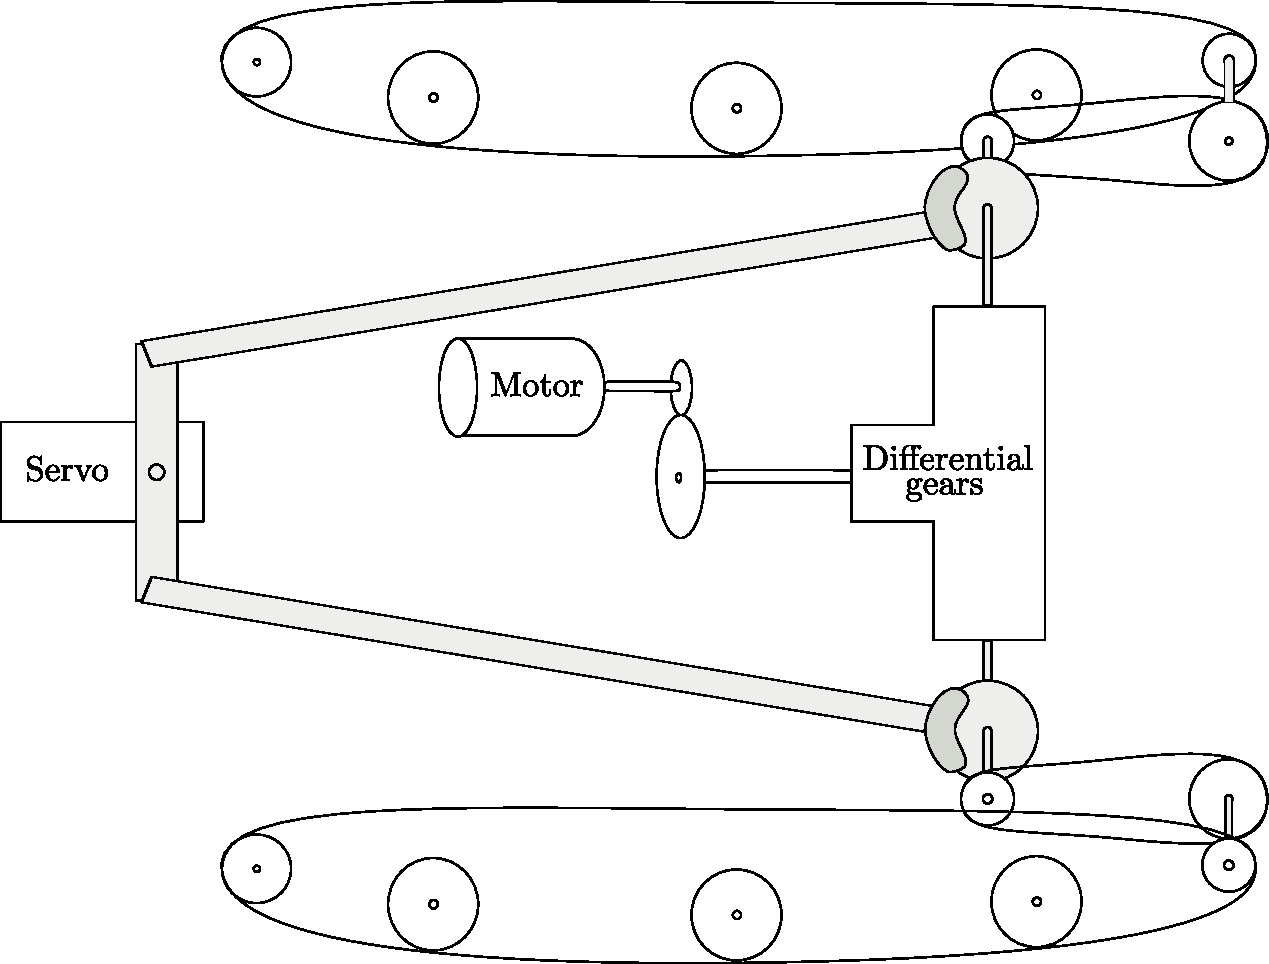
\includegraphics[width=\textwidth]{figures/completeMechanical.pdf}
	\caption{A mechanical diagram of the vehicle}
	\label{fig:completeMechanicalDiagram}
\end{figure}

The \figref{fig:completeMechanicalDiagram} shows both the drivetrain and steering mechanisms on the given vehicle. It is possible to identify and separate these two sub-systems. The driving part allows the vehicle to run and comprises the motor, all the gears that make the belts turn and the belts themselves. On the other hand, the steering part is made of the servomotor which acts on two shafts and breaks one or the other belt, as stated in \secref{sec:Vehicledescription}. In the next sections, the drivetrain, which allows the vehicle to run, and the steering part, which allows the vehicle to turn, are modelled separately, and eventually recombined into a single model.
\section{Velocity model}
This section will contain the modelling of the car.

Plant that we were given, to be able to make requirements.

Black boxing:


\begin{figure}[H]
	\centering
	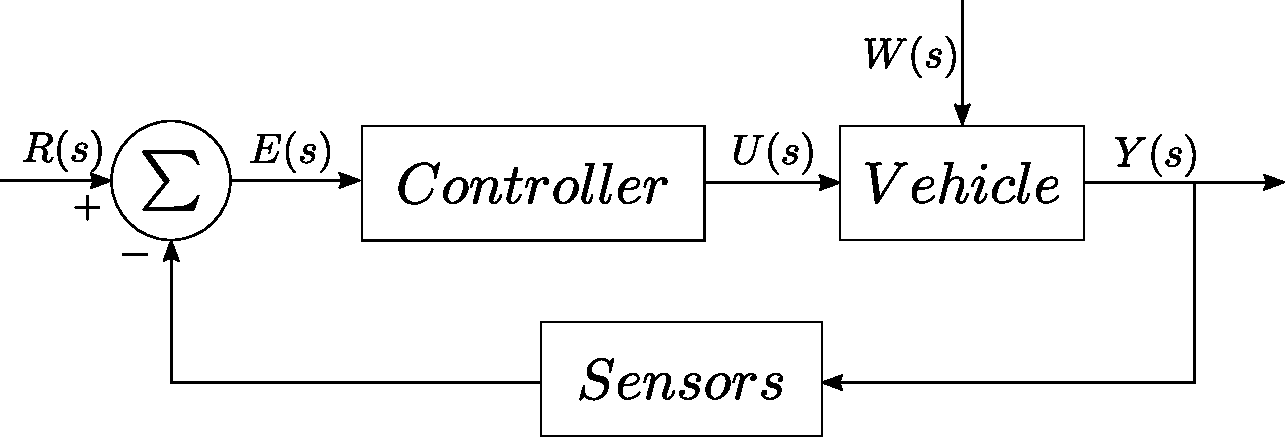
\includegraphics[scale=0.6]{figures/StartTotalModelsystem.pdf}
	\caption{}
	\label{fig:StartTotalModelsystem}
\end{figure}

\subsection{Motor Modelling}\label{motormodelling}
In this section a model of a motor is depicted only as an electrical system, which delivers a rotational force called torque, \si{\tau_m}. The electrical model provides the motor's produced torque to the drivetrain which is further discussed in \secref{DriveTrain}.
%
\subsubsection{Electrical Model}
The output needed from the motor's electrical model is the torque, \si{\tau_m}. To obtain the torque, the formula for translating the electrical current, \si{i_a}, to torque is utilized:
%
\begin{flalign}\centering
  \eq{\tau_m(t)}{K_t \cdot i_a(t)} \unit{N \cdot m}
  \label{equ:motortorque}
\end{flalign}
\hspace{6mm} Where:\\
\begin{tabular}{p{1cm}lll}
& \si{\tau_m(t)} & is the rotational force torque &\unitWh{N \cdot m} \\
& \si{i_a(t)} & is the electrical closed loop current &\unitWh{A}\\
& \si{K_t} & is the motor constant &\unitWh{N \cdot m \cdot A^{-1}}
\end{tabular}

An expression for the current, \si{i_a(t)}, is required to derive a model for the electrical system. In \figref{fig:electricaldiagrammotor} an electrical diagram of the motor is displayed.
%
\begin{figure}[H]
\centering
	\begin{circuitikz}[american voltages]
		\draw
		
		% electromotive force 
		(0,0) to [short] (6,0)
		%to [sV, l=$e_b$] (6,2) %  voltage
		(6,0) to [V, l=$e_b$] (6,3)
		%to node[short]{}(6,2)

		%to node[short]{}(0,0)		 
		(0,0) to [V, l=$U_a$] (0,3) %  voltage

		
		%to [R, l=$Z_G$] (3,3) % generator impedance
		
		(0,3) to [R, l_=$R_a$, i>_=$i_a$] (3,3)	
		
		to [L, l_=$L_a$] (6,3); 
	\end{circuitikz}
  \caption{A electrical diagram of the motor}
  \label{fig:electricaldiagrammotor}
\end{figure}
%
By using Kirchoff voltage law on the closed loop, seen in \figref{fig:electricaldiagrammotor}, an expression including $i_a$ can be derived:
%
\begin{flalign}
\eq{U_a(t)}{R_a \cdot i_a(t) + L_a \cdot \frac{di_a(t)}{dt} + e_b(t)}\unit{V} 
\label{MotorClosedLoop}
\end{flalign}
\hspace{6mm} Where:\\
\begin{tabular}{p{1cm}lll}
& \si{U_a(t)} & is the supply voltage                       &\unitWh{V} \\
& \si{R_a}    & is the internal resistance in the motor     &\unitWh{\Omega}\\
& \si{L_a}    & is the inductance in the motor              &\unitWh{H} \\
& \si{e_b}    & is the electromotive force, also called EMF &\unitWh{V} \\
\end{tabular}

The electromotive force, \si{e_b(t)}, is equivalent to:
%
\begin{flalign}
\eq{e_b(t)}{K_e \cdot \dot{\theta}_m(t)}\unit{V} 
\end{flalign}
\hspace{6mm} Where:\\
\begin{tabular}{p{1cm}lll}
& \si{K_e}            & is the electromotive constant        &\unitWh{Wb} \\
& \si{\dot{\theta}_m(t)} & is the angular velocity in the motor &\unitWh{rad \cdot s^{-1}} \\
\end{tabular}

The equivalent for the electromotive force is substituted into \eqref{MotorClosedLoop}.
%
\begin{flalign}
\eq{U_a(t)}{R_a \cdot i_a(t) + L_a \cdot \frac{di_a}{dt} + K_e \cdot \dot{\theta}_m(t)}&
\end{flalign}
%
The Laplace transform is applied to the derived equation:
%
\begin{flalign}
\eq{U_a(s)}{R_a \cdot i_a(s) + L_a \cdot s \cdot i_a(s) + K_e \cdot \omega_m(s)}&
\end{flalign}
%
The equation is solved for \si{i_a}:
%
\begin{flalign}
\eq{i_a(s)}{\frac{U_a(s) - K_e \cdot \omega_m(s)}{L_a \cdot s + R_a}}&
\end{flalign}
%
By substituting the derived equation for $i_a$ into \eqref{equ:motortorque}, a new expression for the motor's torque is derived. 
%
\begin{flalign}
\eq{\tau_m}{K_t \cdot i_a(s)}&\nonumber\\
\eq{\tau_m}{K_t \cdot \frac{U_a(s) - K_e \cdot \omega_m(s)}{L_a \cdot s + R_a}}
  \label{eq:Totaltorquewithcurrentexpression}
\end{flalign}
%
By dividing with the voltage applied to the motor, $U_a$, a relation can be established:
%
\begin{flalign}
\eq{\frac{\tau_m}{U_a(s) - K_e \cdot \omega_m(s)}}{\frac{K_t}{L_a \cdot s + R_a}}&
  \label{eq:TotaltorquewithcurrentexpressionTransferFunction}
\end{flalign}
%
A relation for the electrical model relative to the motor's torque has been derived. Thus enabling setting up calculations for the vehicle's drivetrain.
\subsection{Drivetrain}\label{Drivetrain}

%% INTRODUCTION %%
The drive train on the given belt vehicle is what translates the torque $\tau_m$ given by the motor into the actual movement of the vehicle. The model of this system part shows the relation between the applied rotational force (or torque) $\tau_m$ and the speed of the belts. It is still considered that the vehicle's tajectory follows a straight line.\\\\
%
Different iterations of this model can be made to get more acuraccy. The first of these iterations should give an overview of how the system reacts to a given torque input. 

%% SSSECTION : BLACK BOX MODEL %%
\subsubsection{Black Box Model}\label{BlackBoxModel}
To get a rough approximation of how the drive train works, a black box model is used. There is a small gear $G_m$ on the motor shaft, which is in contact with another actual gear $G_2$. The imaginary gear $G_d$ represents the differential and the gears and shafts of the drivetrain from (and including) this second gear $G_2$ to the gears that drive the belt, see \figref{fig:DrivetrainMechanicalModel} and \figref{fig:BeltMechanicalDiagram}. The number of teeths on $G_d$ is set to the total gear ratio of this black box

\begin{figure}[H]
	\centering
	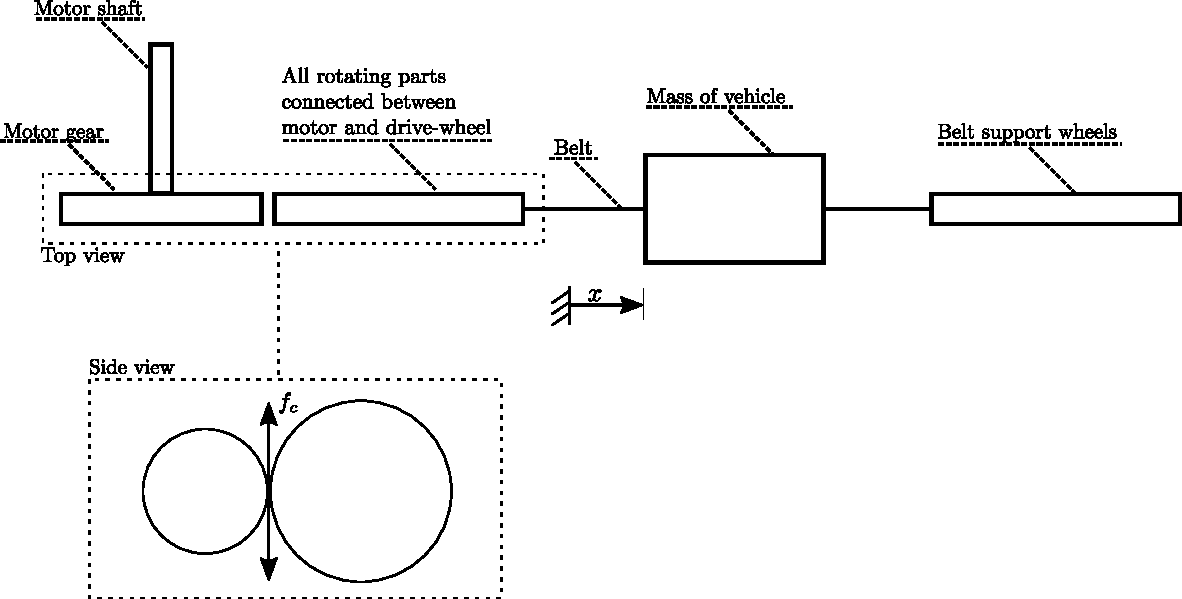
\includegraphics[scale=0.8]{figures/mechanicalDrawing.pdf}
	\caption{A simple mechanical diagram of the vehicle drivetrain}
	\label{fig:DrivetrainMechanicalModel}
\end{figure}
\todo{Add notations to the diagram and create free body diagrams of belt and black box parts}

% APPLICATION OF NEWTON'S SECOND LAW %

\begin{figure}[H]
	\centering
	%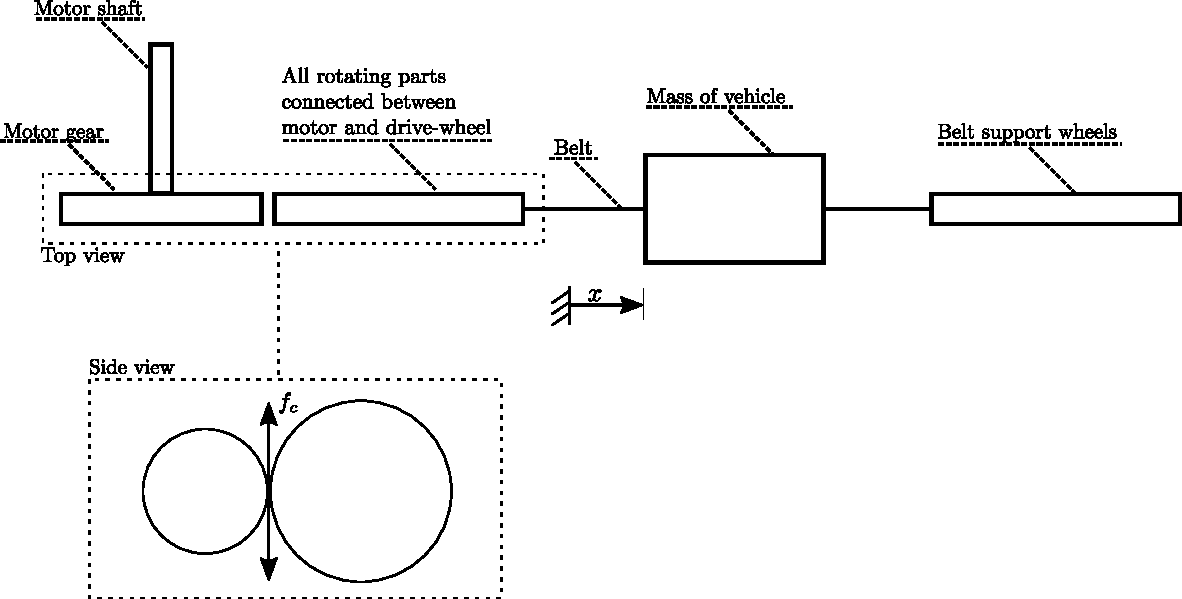
\includegraphics[scale=0.8]{figures/mechanicalDrawing.pdf}
	\caption{A free body diagram of the motor gear}
	\label{fig:MotorGearFreeBodyDiagram}
\end{figure}

\begin{figure}[H]
	\centering
	%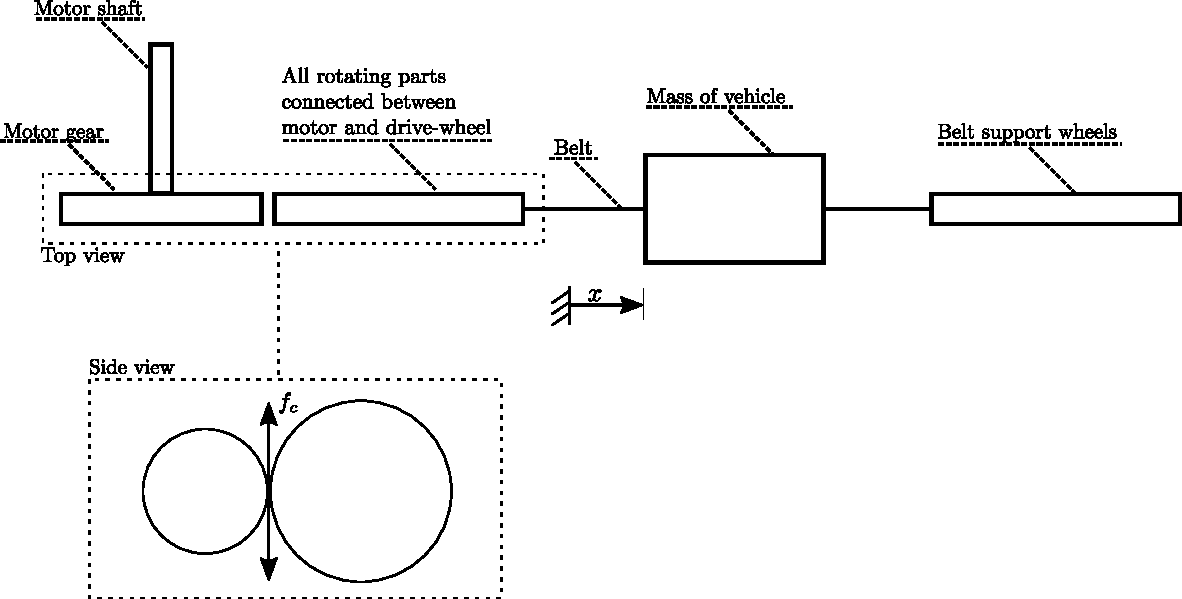
\includegraphics[scale=0.8]{figures/mechanicalDrawing.pdf}
	\caption{A free body diagram of the `black box' gear}
	\label{fig:BlackBoxGearFreeBodyDiagram}
\end{figure}

The \todo{cite equation with label eq:MotorMechaModel from motor modeling part}[EQUATION] is extended with the contribution of the load which is the whole drivetrain. Therefore, from \figref{fig:MotorGearFreeBodyDiagram} and Newton's second law appplied to rotational systems, the following equation can be extracted:
\begin{flalign}\centering
J_m \cdot \dot{\omega}_m(t) = \tau_m(t) - B_m \cdot \omega_m(t) - N_m \cdot f_c(t) 
\label{eq:MotorGearNewtonSecLaw}
\end{flalign}
\hspace{6mm} Where:\\
\begin{tabular}{p{1cm}ll}
& $J_m$ 			      & is the motor's inertia [$kg \cdot m^2$] \\
& $\omega_m$        & is the angular velocity of the motor [$rad \cdot s^{-1}$] \\
& $\dot{\omega}_m$ 	& is the angular acceleration of the motor [$rad \cdot s^{-2}$] \\
& $\tau_m$ 		     	& is the torque delivered by the motor [$N \cdot m$] \\
& $B_m$             & is the coefficient of the friction happening inside the motor [$N \cdot m \cdot s \cdot rad^{-1}$] \\
& $N_m$             & is the number of teeth of the motor gear $G_m$ [$number\ of\ teeths$] \\
& $f_c$             & is the coefficient of the contact force between $G_m$ and $G_d$ [$N \cdot m \cdot number\ of\ teeths^{-1}$]
\end{tabular}

The equation for \figref{fig:BlackBoxGearFreeBodyDiagram} is obtained the same way:
\begin{flalign}\centering
J_d \cdot \dot{\omega}_d(t) = N_d \cdot f_c(t) - N_d \cdot f_b(t)
\label{eq:BlackBoxGearNewtonSecLaw}
\end{flalign}
\hspace{6mm} Where:\\
\begin{tabular}{p{1cm}ll}
& $J_d$ 			      & is the `black box' gear inertia [$kg \cdot m^2$] \\
& $\omega_d$        & is the angular velocity of the `black box' gear [$rad \cdot s^{-1}$] \\
& $\dot{\omega}_d$ 	& is the angular acceleration of the `black box' gear [$rad \cdot s^{-2}$] \\
& $N_d$ 		     		& is the number of teeth on the `black box' gear [$number\ of\ teeth$] \\
& $f_b$             & is the coefficient of the contact force between $G_d$ and the belt [$N \cdot m \cdot number\ of\ teeths^{-1}$] \\
\end{tabular}

%% SSSECTION : BELT MODEL %%
\subsubsection{Belt Model}\label{BeltModel}

\begin{figure}[H]
	\centering
	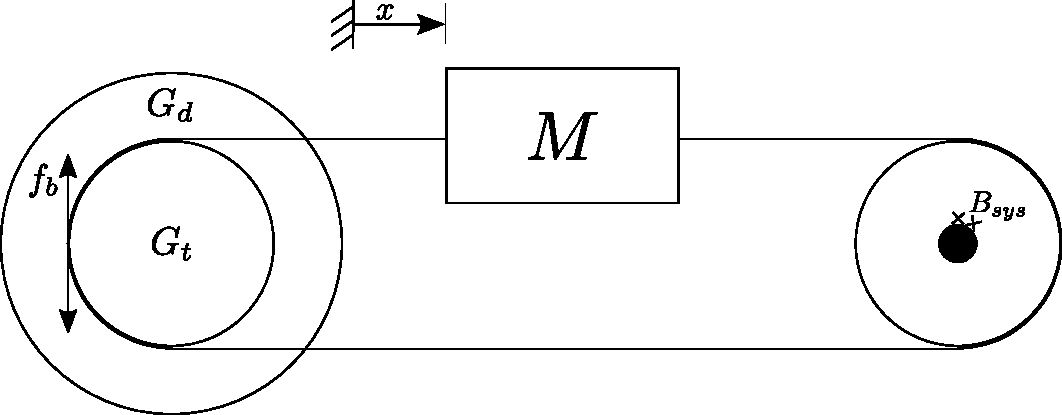
\includegraphics[scale=0.8]{figures/mechanicalDrawingBelt.pdf}
	\caption{A mechanical diagram of the belt part}
	\label{fig:BeltMechanicalDiagram}
\end{figure}

\begin{figure}[H]
	\centering
	% 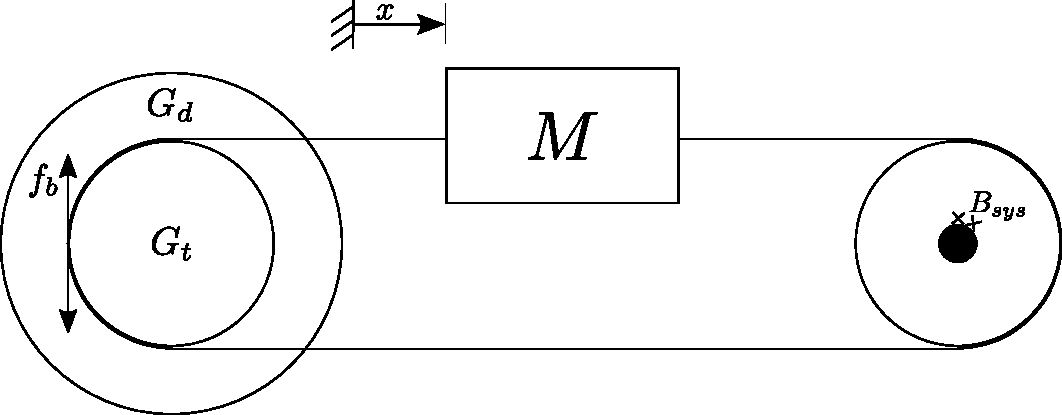
\includegraphics[scale=0.8]{figures/mechanicalDrawingBelt.pdf}
	\caption{A free body diagram of the belt driven mass}
	\label{fig:BeltFreeBodyDiagram}
\end{figure}

From \figref{fig:BeltFreeBodyDiagram}, the mechanical equation of the belt system on \figref{fig:BeltFreeBodyDiagram} is found to be:
\begin{flalign}\centering
M \cdot \dot{v}(t) = r_t \cdot f_b(t) - B_{sys} \cdot v(t)
\label{eq:BeltMassNewtonSecLaw}
\end{flalign}
\hspace{6mm} Where:\\
\begin{tabular}{p{1cm}ll}
& $M$ 			  & is the vehicle's total weight [$kg$] \\
& $v$        	& is the linear velocity of the behicle [$m \cdot s^{-1}$] \\
& $\dot{v}$ 	& is the linear acceleration of the vehicle [$m \cdot s^{-2}$] \\
& $r_t$ 		  & is the translational coefficient between the last gear and the belt [$m \cdot number\ of\ teeths^{-1}$] \\
& $B_{sys}$   & is the coefficient of the friction happening throughout the gears [$N \cdot s \cdot rad^{-1}$] \\
\end{tabular}

The assembling of a model for the drivetrain is made from these separate mechanical equations.

% SSSECTION : ASSEMBLING OF THE DIFFERENT EQUATIONS %
\subsubsection{Drivetrain modeling}\label{DrivetrainModeling}
The combination of \eqref{eq:MotorGearNewtonSecLaw}, \eqref{eq:BlackBoxGearNewtonSecLaw} and \eqref{eq:BeltMassNewtonSecLaw} makes it possible to get the linear velocity of the vehicle $v$ out of the torque $\tau_m$ given by the motor. Indeed, it is possible to link these equations throughout the contact force coefficients $f_c$ and $f_b$.\\\\
%
Taking the Laplace-transform of these equations helps arranging them and eventually, to find a transfer function from $\tau_m(s)$ to $V(s)$ :
%
\begin{flalign}\centering
\eqref{eq:MotorGearNewtonSecLaw} \xRightarrow{\mathcal{L}} J_m \cdot s \cdot \omega_m(s) = \tau_m(s) - B_m \cdot \omega_m(s) - N_m \cdot F_c(s) 
\label{eq:MotorGearNewtonSecLawLaplace}
\end{flalign}
%
\begin{flalign}\centering
\eqref{eq:BlackBoxGearNewtonSecLaw} \xRightarrow{\mathcal{L}} J_d \cdot s \cdot \omega_d(s) = N_d \cdot F_c(s) - N_d \cdot F_b(s)
\label{eq:BlackBoxGearNewtonSecLawLaplace}
\end{flalign}
%
\begin{flalign}\centering
\eqref{eq:BeltMassNewtonSecLaw} \xRightarrow{\mathcal{L}} M \cdot s \cdot V(s) = r_t \cdot F_b(s) - B_{sys} \cdot V(s)
\label{eq:BeltMassNewtonSecLawLaplace}
\end{flalign}
%
By finding the expressions for $F_b$ from \eqref{eq:BeltMassNewtonSecLawLaplace} and then $F_c$ from \eqref{eq:BlackBoxGearNewtonSecLawLaplace}, it is then possible to insert $F_b$ expression into $F_c$'s and the latter into \eqref{eq:MotorGearNewtonSecLawLaplace}.
%
\begin{flalign}\centering
\eqref{eq:BeltMassNewtonSecLawLaplace} \xRightarrow{} r_t \cdot F_b(s) =  M \cdot s \cdot V(s) - B_{sys} \cdot V(s) \xRightarrow{} F_b(s) =  \frac{M \cdot s \cdot V(s) - B_{sys} \cdot V(s)}{r_t}
\label{eq:BeltContactForceLaplace}
\end{flalign} \todo{Get the second implication to be on the next line}
%
And $F_c$ is found this way :
\begin{flalign}\centering
\eqref{eq:BlackBoxGearNewtonSecLawLaplace} \xRightarrow{} N_d \cdot F_c(s) = J_d \cdot s \cdot \omega_d(s) + N_d \cdot F_b(s) \xRightarrow{} F_c(s) =  \frac{J_d \cdot s \cdot \omega_d(s) + N_d \cdot F_b(s)}{N_d} =  \frac{J_d \cdot s}{N_d} \cdot \omega_d(s) + F_b(s)
\label{eq:GearsContactForceLaplace}
\end{flalign}
\todo{Get the steps to be on different lines}
%
Moreover, the relation of velocity for two gears $G_m$ and $G_d$ in contact is given by:
\begin{flalign}\centering
N_m \cdot \omega_m = N_d \cdot \omega_d
\label{eq:GearsVelocityRelation}
\end{flalign}, 

which is equivalent to :
\begin{flalign}\centering
\omega_m = \frac{N_d}{N_m} \cdot \omega_d \xRightarrow{\mathcal{L}} \omega_m(s) = \frac{N_d}{N_m} \cdot \omega_d(s).
\label{eq:BlackBoxGearNewtonSecLaw}
\end{flalign}
%
The same principle is applied from the angular velocity $\omega_d$ to the translational velocity $V$:
\begin{flalign}\centering
v(t) = r_t \cdot \omega_d(t) = r_t \cdot \frac{N_m}{N_d} \cdot \omega_m(t) \xRightarrow{} \omega_m(t) = \frac{N_d}{N_m \cdot r_t} \cdot v(t) \xRightarrow{\mathcal{L}} \omega_m(s) = \frac{N_d}{N_m \cdot r_t} \cdot V(s).
\label{eq:BlackBoxGearNewtonLaplaceNew}
\end{flalign}

It is now possible to replace $\omega_d$ and $F_b$ in \eqref{eq:GearsContactForceLaplace}:
\begin{flalign}\centering
F_c(s) =  \frac{J_d \cdot s}{N_d} \cdot \frac{1}{r_t} \cdot V(s) + V(s) \cdot \left[\frac{M \cdot s + B_{sys}}{r_t}\right] = V(s) \cdot \left[\frac{J_d \cdot s}{r_t \cdot N_d} + \frac{M \cdot s + B_{sys}}{r_t} \right].
\label{eq:GearsContactForceLaplaceNew}
\end{flalign}

And the desired relation between the motor torque and the linear velocity is finally obtained :
\begin{flalign}\centering
\tau_m(s) = J_m \cdot \frac{N_d}{N_m \cdot r_t} \cdot V(s) \cdot s + B_m \cdot \frac{N_d}{N_m \cdot r_t} \cdot V(s) + N_m \cdot \left[\frac{J_d \cdot s}{r_t \cdot N_d} + \frac{M \cdot s + B_{sys}}{r_t} \right] \cdot V(s) = V(s) \cdot \frac{1}{r_t} \cdot \left[\frac{J_m \cdot N_d}{N_m} \cdot s + N_m \cdot J_d \cdot s + M \cdot s + N_m \cdot B_{sys} + B_m \cdot \frac{N_d}{N_m} \right]
\end{flalign}

Therefore, the transfer function from $\tau_m$ to $V$ is :
\begin{flalign}\centering
\frac{V(s)}{\tau_m(s)} = \frac{r_t}{\left[\frac{J_m \cdot N_d}{N_m} + N_m \cdot J_d + M\right] \cdot s + \left[B_{sys} \cdot N_m + B_m \cdot \frac{N_d}{N_m} \right]}
\label{eq:TransferFunctionTorqueToVelocity}
\end{flalign}

Eventually, it is possible to draw a block diagram for the drivetrain, from the motor torque to the vehicle's velocity with \eqref{eq:TransferFunctionTorqueToVelocity} and also back to the angular velocity with \eqref{eq:BlackBoxGearNewtonLaplaceNew}, see .

\begin{figure}[H]
	\centering
	% 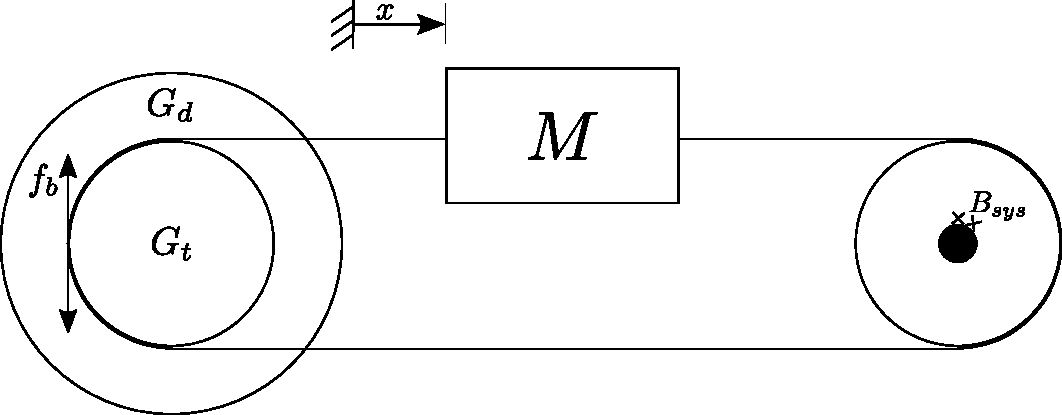
\includegraphics[scale=0.8]{figures/mechanicalDrawingBelt.pdf}
	\caption{A block diagram of the drivetrain}
	\label{fig:BeltFreeBodyDiagram}
\end{figure}
\subsection{Verifying the Velocity Model}


\begin{figure}[H]
  \centering
 	%Trim margins @:   left        bottom       right       top
 	\adjustbox{ trim = {.15\width} {.30\height} {.15\width} {.30\height}, clip }
  {
    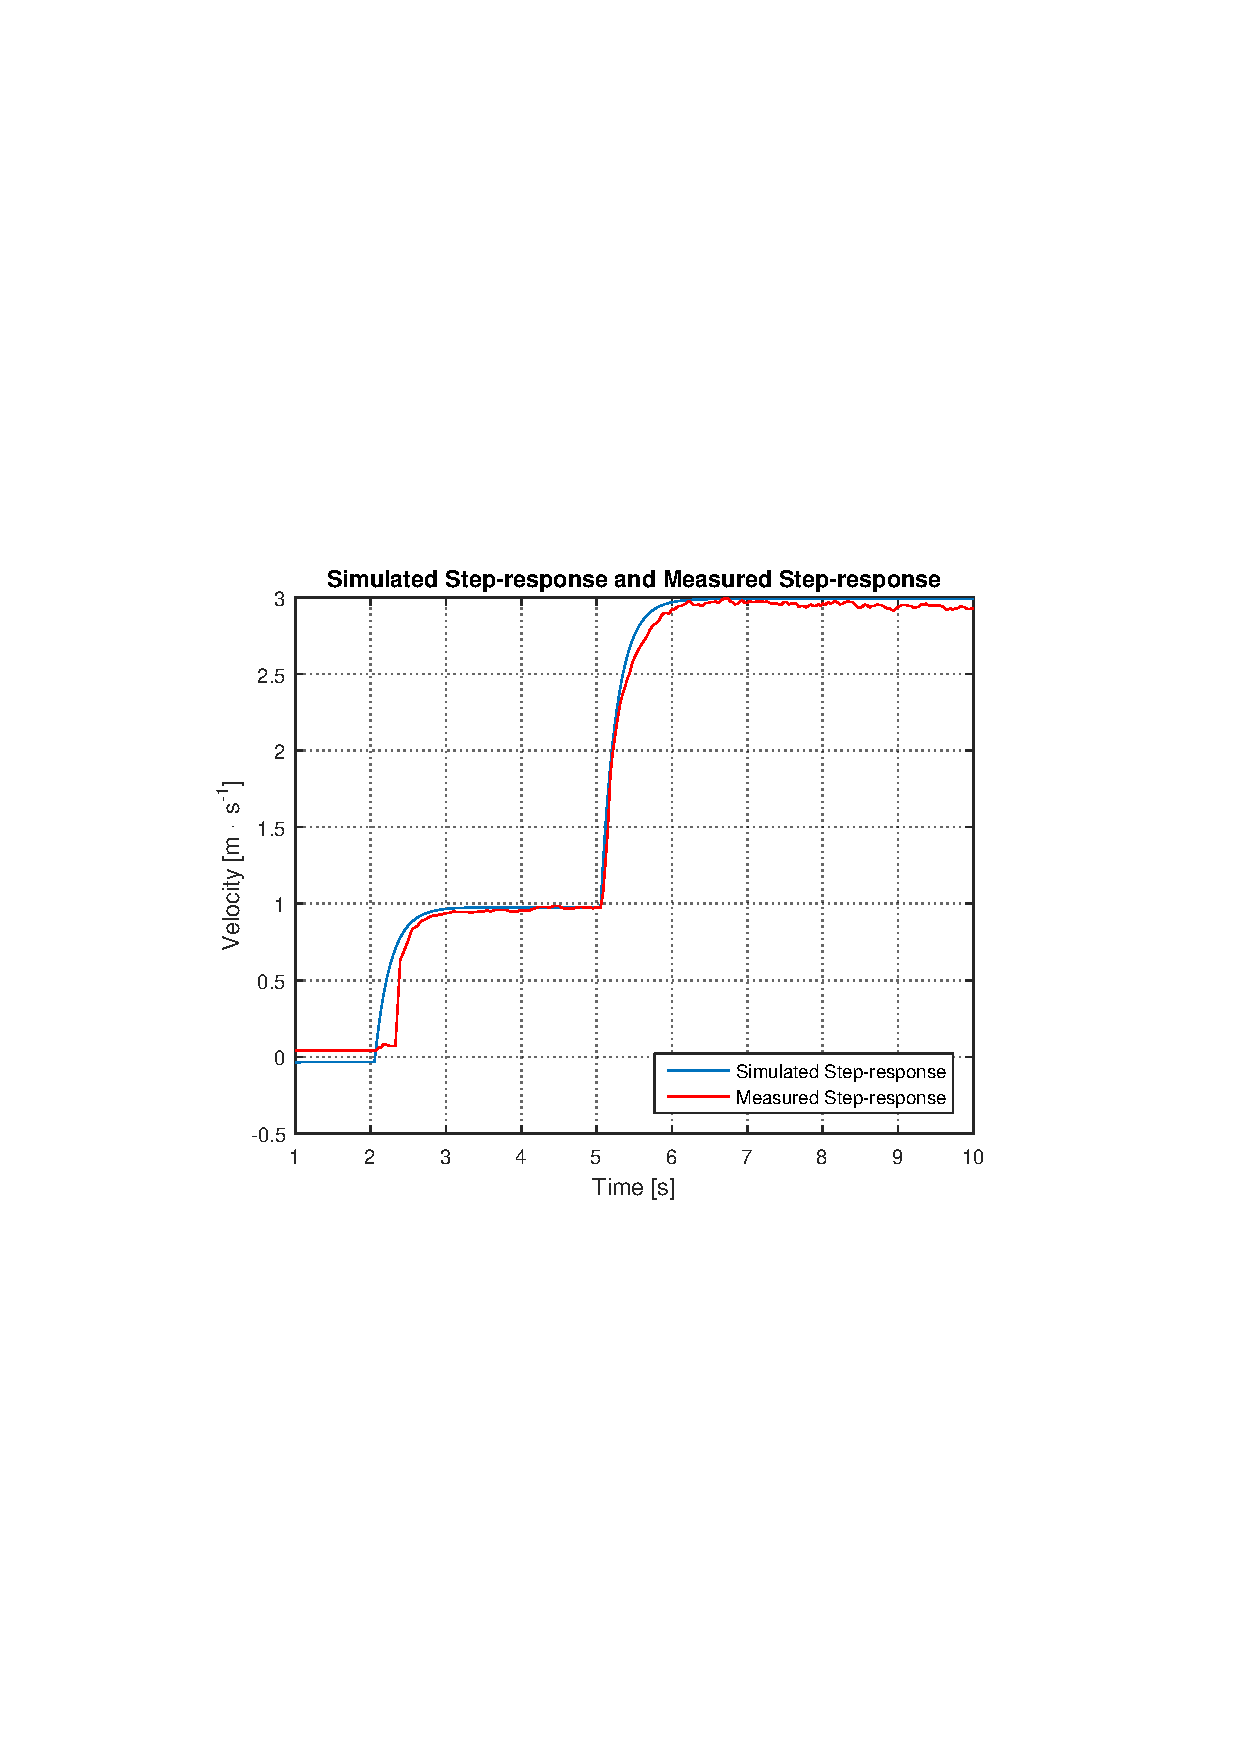
\includegraphics[width=1.2\textwidth]{figures/SimulationIRLsteprespons2.pdf}
  }
  \caption{A plot of a measured armature resistance, with a red line indicating the an average value.}
  \label{armatureResistance}
\end{figure}


\section{Steering Model of the Vehicle}\label{sec:SteeringModel}
After describing a model for the driving part of the vehicle seen on \figref{fig:completeMechanicalDiagram}, the present section draws a model from the steering part, which is isolated in \figref{steeringMechanical}. Thus, the focus is made on the relationship between the PWM command signal to the servo, the angle of the servo, and the resulting orientation of the vehicle. To facilitate the steering modelisation, the vehicle's velocity is considered only around an operating point. A overview of the braking system can be seen in.

 \begin{figure}[H]
 	\centering
 	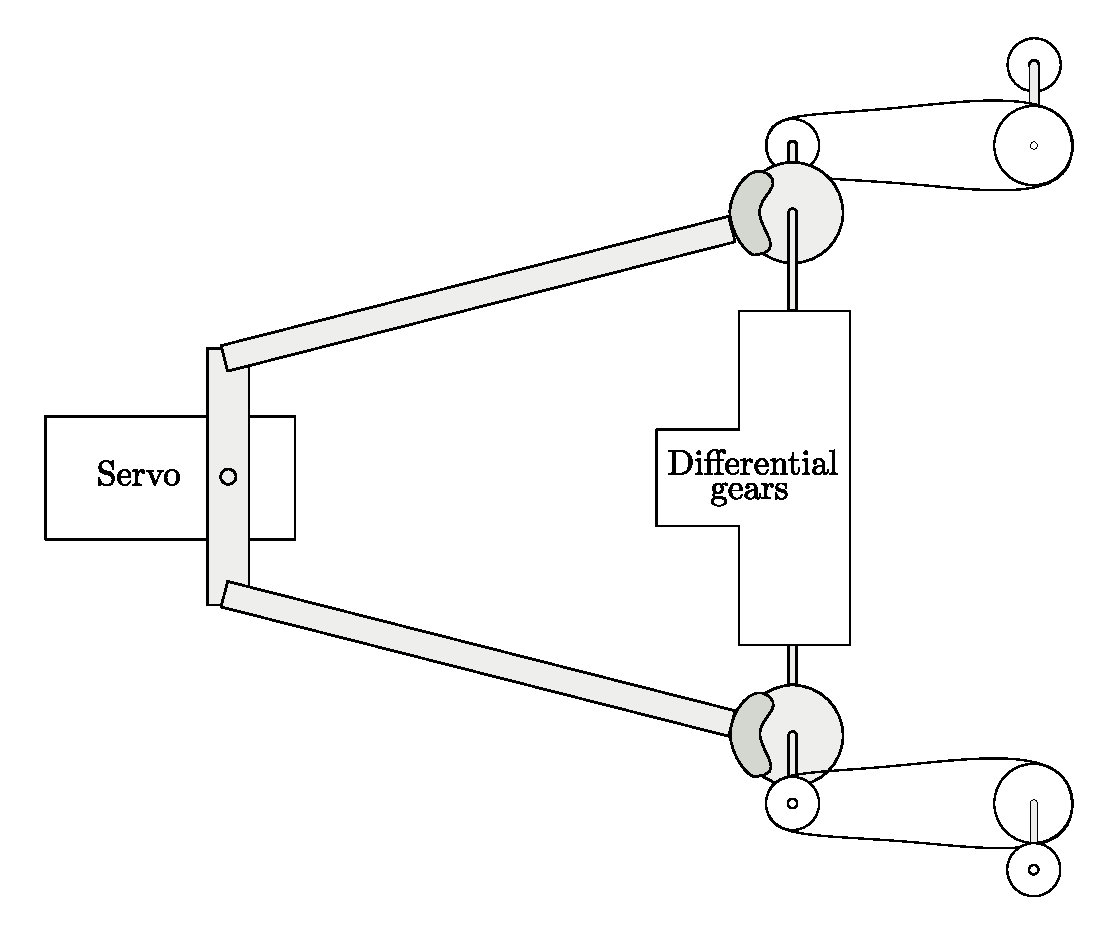
\includegraphics[scale=0.6]{figures/steeringMechanical.pdf}
 	\caption{Mechanical drawing of the steering}
 	\label{steeringMechanical}
 \end{figure}

As described in \secref{sec:Vehicledescription}, when the servo turns one way, it pushes one of the arms, which in turn moves  a brake pad towards the brake disc to add friction and hold the corresponding belt. The differential gears will then transfer the power from one belt to the other, making the vehicle turn.

\subsection{Directional model}
As the steering system contains many moving parts, it is convenient to start with a simple model, to verify it, and iterate until it is satisfactory.\\
%
The first model considered can be seen on \figref{basicSteering}.

\begin{figure}[H]
	\centering
	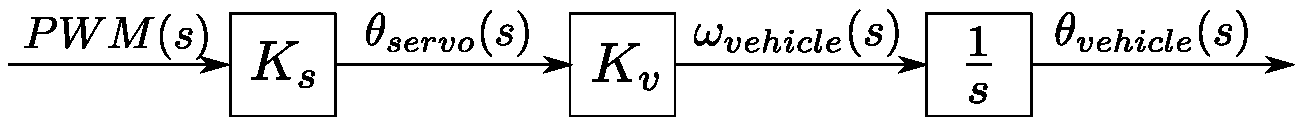
\includegraphics[width=0.8\textwidth]{figures/basicSteeringModel.pdf}
	\caption{A basic steering model}
	\label{basicSteering}
\end{figure}
 
As described in \secref{Servo}, the angle of the servo is proportional to a pulse width modulated signal on its control input (let aside the intrinsic offset of the servomotor). The pulse width is therefore chosen as the input in this model. It is then multiplied by a constant, \si{K_s}, which translates the pulse width to an angle of the servo.
Since the velocity of the vehicle is assumed constant, the rate of change of the direction, \si{\omega_{v} (s)}, must be a function of the servo angle, and a constant, \si{K_v}, representing the speed of the vehicle and the braking the system.
The rate of change in the vehicle's angle is finally integrated over time, resulting in a angle heading, \si{\theta_{v} (s)}. 

\subsection{Extension of the Directional Model}

The first model describes in a simple manner how the mechanical part of the steering system functions. However, it can be extended to include the time delay caused by the servo. According to \secref{Servo}, the servo is controlled by a PWM signal with a period of 30 ms. This means, that it will not be possible to update the servo angle continuously, but only in discrete time steps of 30 ms. These steps will be implemented in the model as a sampling delay.\\
As seen in the Modeling and Control course on the 5th semester of Electronic and IT at Aalborg University \cite{KMNielsen}, the delay of a signal, \si{u(t)}, is usually described in frequency domain by an exponential factor:
\begin{flalign}
  \eq{\mathcal{L}\left[u(t+\lambda)\right]}{U(s)\cdot e^{-\lambda \cdot s}}&&\nonumber
  \label{eq:delaySampling}
\end{flalign}
However, for small values of \si{\lambda}, it is possible to use the approximation:
\begin{flalign}
  \si{\exp(-\lambda \cdot s) \simeq \frac{1}{\lambda\cdot\text{s}+1}}&&\nonumber
  \label{eq:delaySampling}
\end{flalign}

With the delay from the servo, \si{\lambda}, being \si{30\ ms}, this approximation is used and inserted into the model between the sent PWM and the action of the servo, as shown on \figref{basicSteeringWithDelay}:
\begin{figure}[H]
	\centering
	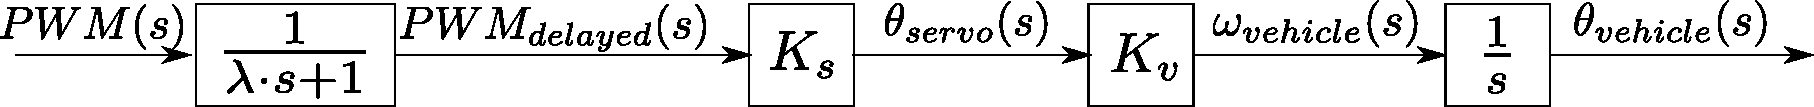
\includegraphics[width=\textwidth]{figures/basicSteeringModelWithDelay.pdf}
	\caption{A basic steering model}
	\label{basicSteeringWithDelay}
\end{figure}
%
This model describes the action of the steering on the vehicle, by translating PWM signals sent to the servo into headings of the vehicle. It allows to apply a control on the direction of the vehicle, but not for it to follow a predefined set of points.

\subsection{Line Following Model}
Since the vehicle has to follow a predetermined route, a direction control alone is not enough. As seen on \figref{SteeringDeviation}, any change of direction caused by a disturbance, will cause a deviation from the planned line between two points A and B on the wanted route. This is why a model of this deviation is created in this section.

\begin{figure}[H]
	\centering
	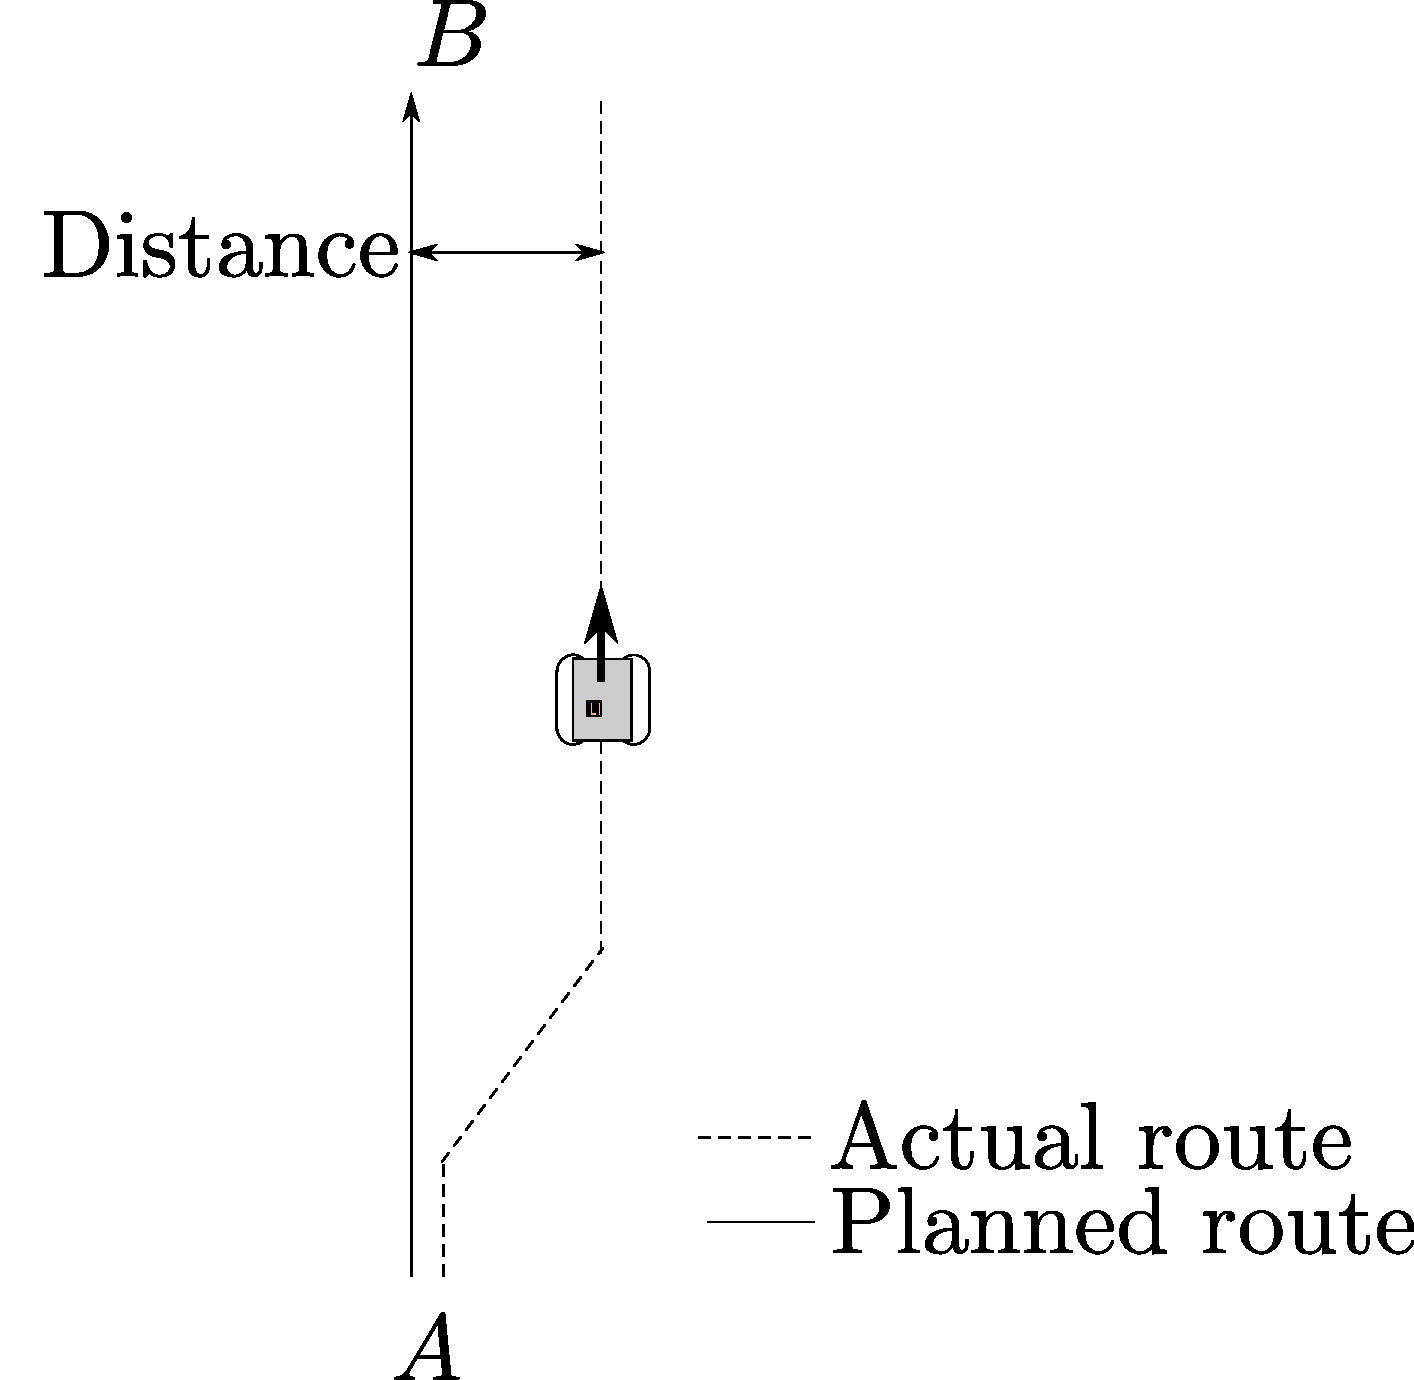
\includegraphics[width=0.6\textwidth]{figures/steeringDeviation.pdf}
	\caption{Consequence of using directional control alone}
	\label{SteeringDeviation}
\end{figure}

How large the deviation is, should depend on the vehicle's erroneous angle from the wanted line, its velocity and the time it takes for the control system to account for the error. The instantaneous distance, \si{d_1}, can be expressed with simple trigonometry as:
\begin{flalign}
  \eq{d_1}{v_1 \cdot t_1 \cdot \sin\left(\Delta\theta_1\right)}\unit{m}
  \label{eq:distance}
\end{flalign}
\hspace{6mm} Where:\\
\begin{tabular}{p{1cm}lll}
  &\si{d_1}   & is the distance of the vehicle from the wanted line at instant \si{t_1} &\unitWh{m}\\
  &\si{t_1}   & is the time instant of measurement                                      &\unitWh{s}\\
  &\si{v_1}   & is the vehicle's velocity at instant \si{t_1}                           &\unitWh{m \cdot s^{-1}}\\
  &\si{\Delta\theta_1}  & is the vehicle's angle compared to the wanted line  at instant \si{t_1} &\unitWh{rad}\\
\end{tabular}

The speed is assumed to be constant. From this assumption, the distance error over time, \si{d(t)}, is then described as an integration over time of the sine of the error angle multiplied with the velocity, see \eqref{eq:angleIntegration}.
\begin{flalign}
  \eq{d(t)}{v \cdot \int^{t} \sin\left(\Delta\theta (t)\right) \mathrm{d}t}\unit{m}
  \label{eq:angleIntegration}
\end{flalign}
\hspace{6mm} Where:\\
\begin{tabular}{p{1cm}lll}
  &\si{d(t)}        & is the distance of the vehicle from the wanted line &\unitWh{m}\\
  &\si{t}           & is the time variable used for the integral          &\unitWh{s}\\
  &\si{v}           & is the constant vehicle's velocity                  &\unitWh{m \cdot s^{-1}}\\
  &\si{\Delta\theta (t)}  & is the vehicle's angle compared to the wanted line  &\unitWh{rad}\\
\end{tabular}

The integration over time actually multiplies the integrated sine function with a time interval. Moreover, the sine function output being dimensionless, the resulting function, \si{d(t)}, has the dimension of a length and the unit of meters: it is the time varying distance between the vehicle and the wanted line.\\
To facilitate the process of Laplace transform, it is necessary to linearize the \si{\sin} function. By assuming that the vehicle is in its operating point, i.e. within a short distance and small angle from the wanted line, the angle difference, \si{\Delta\theta (t)}, is then very small. For small angle values, the \si{\sin} function can be approximated to :
\begin{flalign}
  \si{\sin\left(\Delta\theta\right) \simeq \Delta\theta}&&\nonumber
\end{flalign}
%
Thus, the \eqref{eq:angleIntegration} is simplified into:
\begin{flalign}
  \eq{d(t)}{v \cdot \int^{t} \Delta\theta (t) \mathrm{d}t}\unit{m}
  \label{eq:angleIntegrationLinearized}
\end{flalign}
%
The transformation of \eqref{eq:angleIntegration} into the Laplace domain eventually yields:
\begin{flalign}
  \eq{D(s)}{v \cdot \frac{1}{s} \cdot \Delta\theta (s)}\unit{m}
\end{flalign}
By definition, \si{\Delta\theta} is the difference between the real heading of the vehicle, \si{\theta_v}, and the reference angle, \si{\theta_{ref}}. Since both angles are given or measured in degrees, it is also needed to convert them to radians to match the units, as shown in \eqref{eq:angleIntegrationLaplace}.
\begin{flalign}
  \eq{D(s)}{\frac{\pi}{180} \cdot v \cdot \frac{1}{s} \cdot \left(\theta_{v}(s) - \theta_{ref}(s)\right)}\unit{m}
  \label{eq:angleIntegrationLaplace}
\end{flalign}
\hspace{6mm} Where:\\
\begin{tabular}{p{1cm}lll}
  &\si{\theta_{v}(s)} & is the absolute real heading of the vehicle &\unitWh{^{\circ}}\\
  &\si{\theta_{ref}(s)}     & is the absolute wanted heading of the vehicle &\unitWh{^{\circ}}\\
\end{tabular}

From \eqref{eq:angleIntegrationLaplace}, the block diagram of the steering model on \figref{basicSteeringWithDelay} can be extended, as seen on \figref{fig:steeringLineFollowingModel}.

\begin{figure}[H]
  \centering
  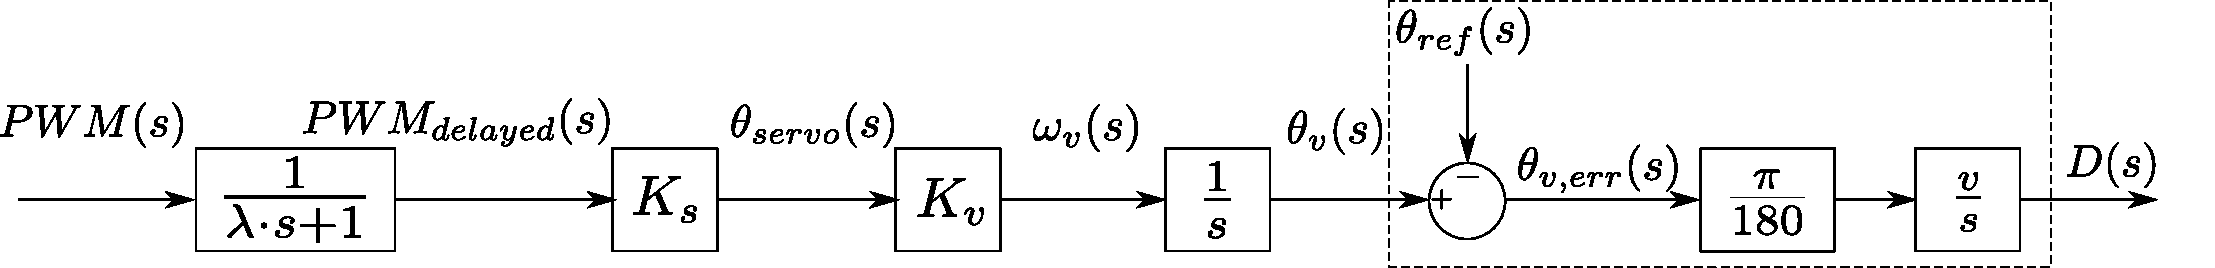
\includegraphics[width=1\textwidth]{figures/steeringModelWithLineFollowing.pdf}
  \caption{Block diagram of the combined directional and line following models}
  \label{fig:steeringLineFollowingModel}
\end{figure}

This model describes how the steering reacts and therefore, how the vehicle can be moved sideways. It allows for the controlling of both the heading of the vehicle and its position relative to the line it has to follow, see \secref{sec:steeringController}.\\
However, it also uses assumptions that need to be verified. Firstly, the distance calculation model only works if the vehicle is deviating and not if it is following a line parallel to the wanted one. Indeed, were that the case, then the angle difference would approach zero and the calculated distance too, even though it wouldn't actually be. This problem is considered in \todo{secref{sec:lineFollowingControl}}. Moreover, this model is only used to simulate the system's behavior since the distance calculations are made with the use of the Games on Track positioning system. Finally, the velocity can only be considered constant if properly controlled, as done in \secref{sec:velocityController}.

%%% Part 2 %%%
\part{Design \& implementation}

%%% Part 3 %%%
\part{Test \& conclusion}


%%% Setup for Appendix and Bibliography %%%
\bookmarksetup{startatroot} %this is it
\addtocontents{toc}{\bigskip} %perhaps as well
\newpage
\fancyhead[RO]{\color{aaublue}\small Appendix \nouppercase\rightmark} %even page - chapter title
\fancyhead[LE]{\color{aaublue}\small Appendix \nouppercase\rightmark} %uneven page - section title
\fancyhead[RE,LO]{}
\titleformat{\section}[hang]{\Large\bfseries}{\thesection\hsp\textcolor{aaublue}{|}\hsp}{0pt}{\Large\bfseries}
\renewcommand{\thesection}{\Alph{section}}
\setcounter{section}{0}

%%% Appendix %%%
\chapter*{Appendix}
\addcontentsline{toc}{chapter}{Appendix}

%---------- Appendix A ---------------------------------------- GoT Description
\section{The Games on Track GT-position system}
The Games on Track GT-Position system, shortened GoT, is a GPS system which uses radio-waves and ultrasound to locate the object. The system is build up by three hardware components, the transmitter, receiver and master. 

\subsubsection{Transmitter}
The transmitter component is placed on the object, which needs to be located. To indicate the objects position, the transmitters emits out ultrasound waves to indicate where it and the object is positioned. The transmitter component runs on 2 AA-batteries and therefore does not need an external power-source. 

\subsubsection{Receiver}
\todo{What kind of "radio waves" does the receiver transmit data to the master?}
The receiver component is placed around the area where the object, with the transmitter, has to be located. The receivers assignment is to search for the ultrasound waves, which the transmitter is emitting. The ultrasound waves received by the receivers, provides information containing the distance between the specific receiver to the transmitter located on the object. To be able to calculate the exact position of the transmitter and the object, a minimum of three receivers is necessary. however, more receivers can be added to the system for more reliability and the ability to cover a larger area. For the receivers to work at a high efficiency, they should be placed 1 to 2 meters apart and not on a single line. But if receivers shall cover a bigger area, they can be placed up to a distance of 5 meters between them, however, this would affect the measurement and thereby make it less reliable. Each receiver have a maximum range of 8 meters and as seen on \figref{receiverSetup}, the three receivers should be placed in each others reach. The receivers needs between 14 to 20 volt DC. Thus, making the receivers able to be powered through a computer charger if necessary.

\begin{figure}[H]
	\centering
	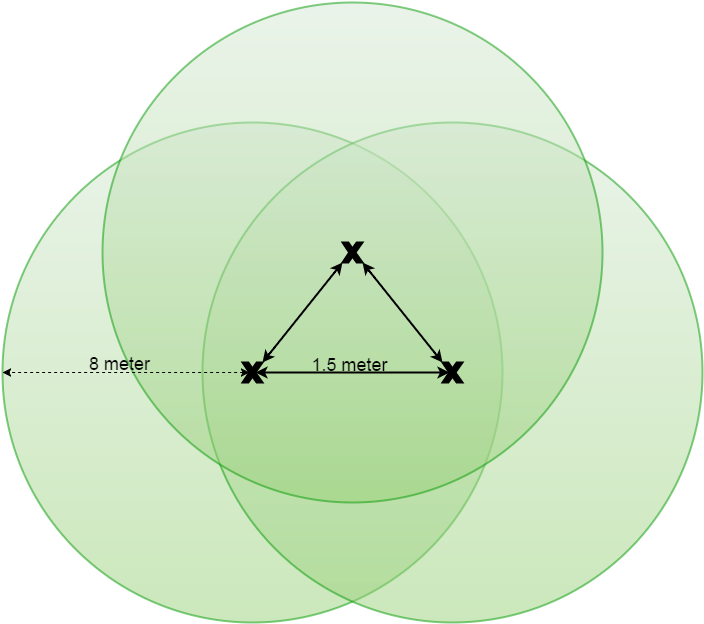
\includegraphics[scale=0.5]{figures/ReceiverSetup.png}
	\caption{Example on a standard setup for the receivers (increase size of text in figure)}
	\label{receiverSetup}
\end{figure}

\subsubsection{Master}
The master is a receiver which should be connected to a computer. The masters assignment is to receive the data transmitted from the individual receivers and send it directly to the connected computer. The master is powered through a USB cable, between the master and the computer.
\subsubsection{Computer}

The program on the computer, which handles the information received from the master, uses the data to calculate the position of the transmitter. This is done with a method call Trilateration. Trilateration is a way of calculating a position, in a three-dimensional space, from three distances (from known locations), with the help of spheres, circles and triangles. Therefore it is necessary for the system to have atleast three receivers, as mentioned earlier. With additional receivers a check up can be performed to ensure the position of the transmitter is correct.\\\\

If the receivers have been moved, it is necessary to calibrate the system. This is done with a calibration triangle. The calibration triangle is three markings on the surface, that will be setup to be the zero surface for the Z-axis. One of the points on the calibration triangle is made the origin (0,0,0) of the coordinate system. Another point on the triangle will then be call (X,0,0), in which the line between the first point and the second point will become the X-axis. The last point will be call (X,Y,0) and will determine in which way the positive Y-axis will go. The surface which the calibration triangle is creating, will be the zero surface for the Z-axis, and is horizontal. The distance between the three points is measured and put into the software. Thereafter, with using the transmitter, are the position of the receivers calculated.  The transmitter is first placed in the first point (0,0,0), there next the second point (X,0,0) and then in the last point (X,Y,0). At each point the distance to the receivers is measured. Out from this data, about the placement of the points and their distance to the receivers, the software can calculate the position of each receiver, with the help of trilateration. \\\\

\todo{How should the recievers be placed? how far can they reach, picture?}

\todo{How do you calibrate, do you move the transmitter around?? but that in the text}

\todo{mergeconflict which needs to be addressed}

The program on the computer, which handles the information received from the master, uses the data to calculate the position of the transmitter. This is done with a method call Trilateration. Trilateration is a way of calculating a position, in a three-dimensional space, from three distances (from known locations), with the help of spheres, circles and triangles. Therefore it is necessary for the system to have atleast three receivers, as mentioned earlier.  With additional receivers a check up can be performed to ensure the position of the transmitter is correct. Trilateration does not work, if the three know points is on a single line and therefore shall the receivers be placed in a triangle.\\\\
\noindent
If the receivers have been moved, it is necessary to calibrate the system. This is done with a calibration triangle. The calibration triangle is made of three points on a flat surface and have a distance of 40 to 200 centimeters between them. One of the points on the calibration triangle is made the origin (0,0,0) of the new coordinate system. Another point on the triangle will then be call (X,0,0), in which the line between the first point and the second point will become the X-axis. The last point will be call (X,Y,0) and will determine in which way the positive Y-axis will go. The surface which the calibration triangle is placed on, will be the XY-plan, where Z will go positiv in the direction of the receivers. The distance between the three points is measured and put into the program. Thereafter, the transmitter placed in the three point, with (0,0,0) first and (X,Y,0) last. When the transmitter is placed in a point, the receivers measure the distance between them and the transmitter. From the data, the program can calculate the position of each receiver, with the help of trilateration. \\\\


%---------- Appendix B ---------------------------------------- Motor Tests
\pagebreak
\section{Motor Tests}
\nopagebreak
\subsection{Armature Resistance} %\label{put a label here and uncomment}
\textbf{Name: Group 510}\\
\textbf{Date: 30/09 - 2015}

\subsubsection{Purpose}
The purpose of the test is to measure the armature resistance $R_a$ of the motor.

\subsubsection{Setup}
\begin{figure}[H]
  \centering
	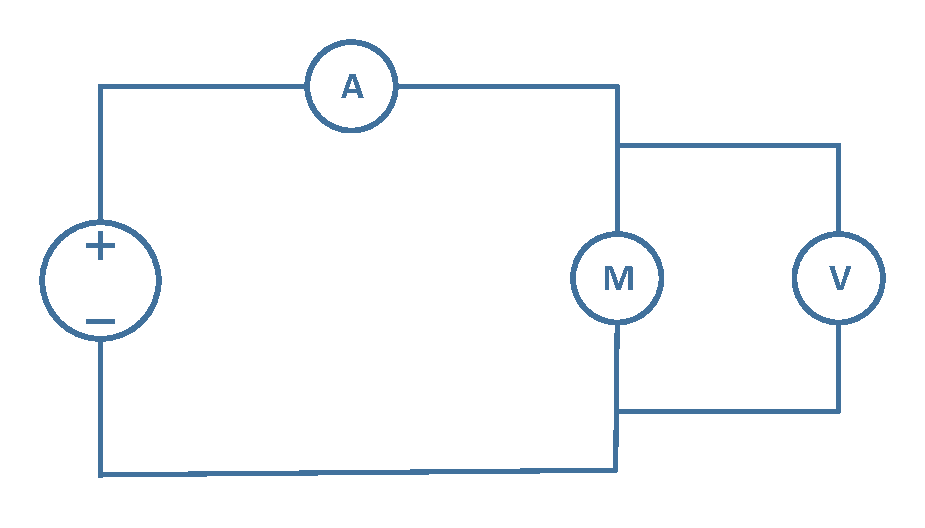
\includegraphics[scale=0.5]{figures/MotorTest1.pdf}
	\caption{Setup diagram}
\end{figure}

\subsubsection{List of Equipment}
\begin{table}[H]
\begin{tabular}{|l|l|p{4cm}|}
\hline%------------------------------------------------------------------------------------
  \textbf{Instrument}                        &  \textbf{AAU-no.}  &  \textbf{Type}       \\
\hline%------------------------------------------------------------------------------------
  Multimeter 1                               &  60764             &  Fluke 189 True RMS  \\
\hline%------------------------------------------------------------------------------------
  Multimeter 2                   		         &  60769             &  Fluke 189 True RMS  \\
\hline%------------------------------------------------------------------------------------
  Power Supply \small{(0 - 32 V) (0 - 10 A)} &  77076             &  Ea - ps 7032 - 100  \\
\hline%------------------------------------------------------------------------------------
  Clamp for fixing the motor                 &  03039             &                      \\
\hline%------------------------------------------------------------------------------------
\end{tabular}
\end{table}

\subsubsection{Procedure}

\begin{enumerate}
  \item Turn on the two multimeters and choose Voltage and Ampere settings respectively.
  \item Fix the motor shaft so it can not turn.
  \item Choose the first current value ($0,5$ A) on the current limiting of the power supply.
  \item Turn on the power supply and adjust the current limiting in accordance with the ampere meter.
  \item Read the voltage supplied to the motor from the volt meter.
  \item Repeat the three previous steps for each measurement in $0,5$ A increments up to $5$ A.
  \item Switch the poles of the power supply and repeat the measurements in the negative direction.
\end{enumerate}

\subsubsection{Results}

\begin{table}[H]
\begin{tabular}{|l|l|l| l|l|}
\cline{1-2}\cline{4-5}%-----------------------             ----------------------------------------------
  \textbf{Input (A)}   & \textbf{Output (V)} &\phantom{hey}& \textbf{Input (A)}   & \textbf{Output (V)}\\
\cline{1-2}\cline{4-5}%-----------------------             ----------------------------------------------
  $-5,0$               &            $-0,71$  &             & $0,5$                & $0,16$             \\
\cline{1-2}\cline{4-5}%-----------------------             ----------------------------------------------
  $-4,5$               &            $-0,65$  &             & $1,0$                & $0,34$             \\
\cline{1-2}\cline{4-5}%-----------------------             ----------------------------------------------
  $-4,0$               &            $-0,59$  &             & $1,5$                & $0,53$             \\
\cline{1-2}\cline{4-5}%-----------------------             ----------------------------------------------
  $-3,5$               &            $-0,54$  &             & $2,0$                & $0,62$             \\
\cline{1-2}\cline{4-5}%-----------------------             ----------------------------------------------
  $-3,0$               &            $-0,43$  &             & $2,5$                & $0,64$             \\
\cline{1-2}\cline{4-5}%-----------------------             ----------------------------------------------
  $-2,5$               &            $-0,36$  &             & $3,0$                & $0,75$             \\
\cline{1-2}\cline{4-5}%-----------------------             ----------------------------------------------
  $-2,0$               &            $-0,27$  &             & $3,5$                & $0,78$             \\
\cline{1-2}\cline{4-5}%-----------------------             ----------------------------------------------
  $-1,5$               &            $-0,20$  &             & $4,0$                & $0,80$             \\
\cline{1-2}\cline{4-5}%-----------------------             ----------------------------------------------
  $-1,0$               &            $-0,14$  &             & $4,5$                & $0,83$             \\
\cline{1-2}\cline{4-5}%-----------------------             ----------------------------------------------
  $-0,5$               &            $-0,07$  &             & $5,0$                & $0,88$             \\
\cline{1-2}\cline{4-5}%-----------------------             ----------------------------------------------
\end{tabular}
\end{table}

\begin{figure}[H]
  \centering
 	%Trim margins @:   left        bottom       right       top
 	\adjustbox{ trim = {.15\width} {.30\height} {.15\width} {.30\height}, clip }
  {
    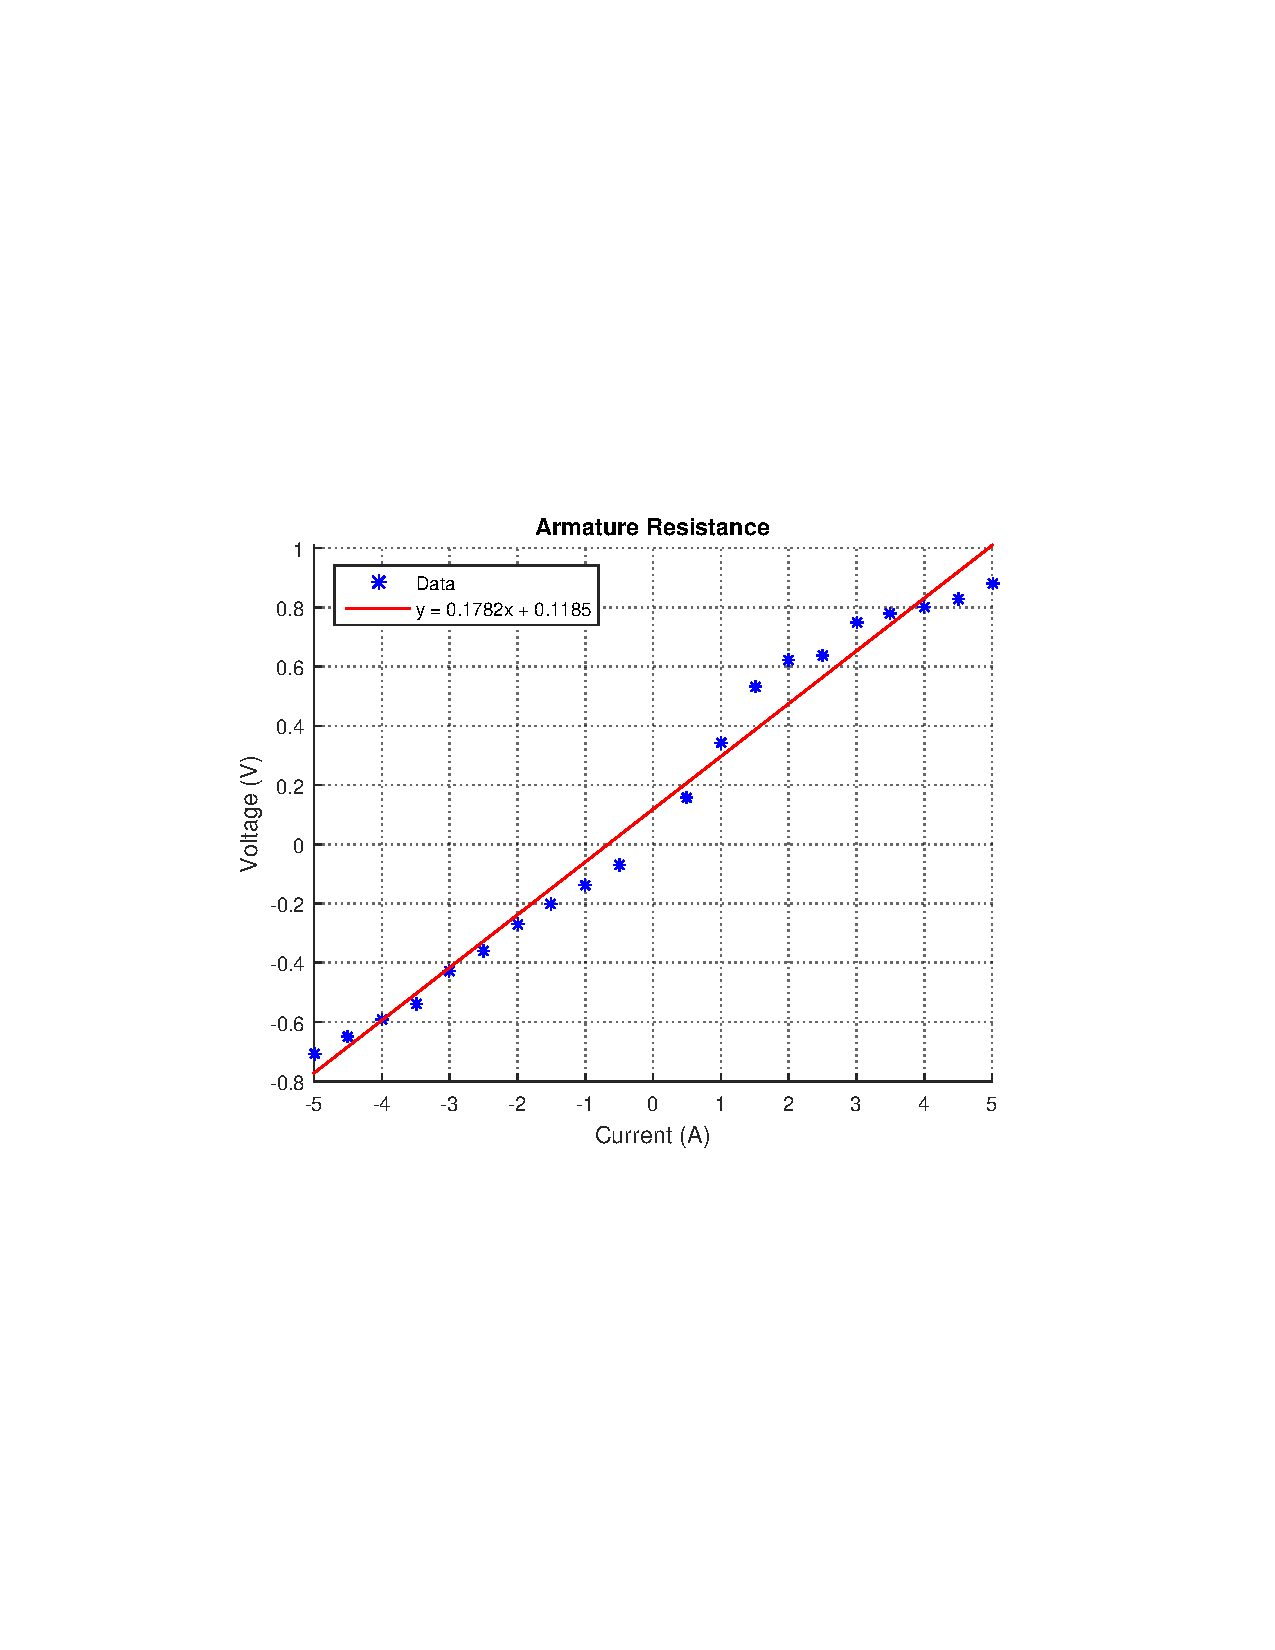
\includegraphics[width=\textwidth]{figures/armatureResistance.pdf}
  }
  \caption{A plot of a measured armature resistance, with a red line indicating the an average value.}
  \label{armatureResistance}
\end{figure}

During these measurements the motor is in steady state. This is necessary for the inductor in the armature coil to act as a short circuit, which allows easy calculation of the armature resistance. In steady state we get:

\begin{flalign}
  \eq{R_a} {\frac{U_a}{I_a}} \unit{\Omega}\nonumber
\end{flalign}
\hspace{6mm} Where:\\
\begin{tabular}{p{1cm}lll}
  & \si{I_a} & is the armature current    &\unitWh{A}    \\
  & \si{U_a} & is the armature voltage    &\unitWh{V}    \\
  & \si{R_a} & is the armature resistance &\unitWh{\Omega}  \\
\end{tabular}

As seen on the data plot in \figref{armatureResistance} the result is a relatively linear function. The armature resistance is approximated directly as the slope of the least square line: \todo{is it not invers?}
\begin{flalign}
  \eq{R_a}{0,178}\ \si{\Omega}&\nonumber
\end{flalign}
\pagebreak
\subsection{Armature Inductance}%\label{put a label here and uncomment}
\textbf{Name: Group 510}\\
\textbf{Date: 30/09 - 2015}

\subsubsection{Purpose}
The purpose of the test is to determine the Armature inductance \si{L_a} of the motor.

\subsubsection{Setup}
\begin{figure}[H]
  \centering
	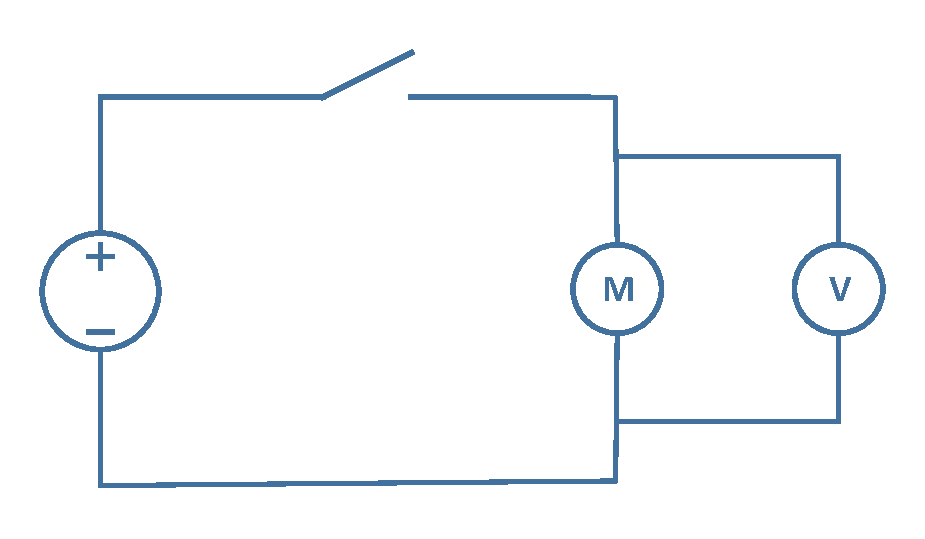
\includegraphics[scale=0.5]{figures/MotorTest2.pdf}
	\caption{Setup diagram}
\end{figure}

\subsubsection{List of Equipment}

\begin{table}[H]
\begin{tabular}{|l|l|p{4cm}|}
\hline%--------------------------------------------------------------------------------
  \textbf{Instrument}                    &  \textbf{AAU-no.}  &  \textbf{Type}       \\
\hline%--------------------------------------------------------------------------------
  Power Supply ($0 - 32$ V) ($0 - 10$ A) &  77076             &  Ea - ps 7032 - 100  \\
\hline%--------------------------------------------------------------------------------
  AC/DC Current Clamp (Output: 100 mV/A) &  78550             &  FLUKE i30s          \\
\hline%--------------------------------------------------------------------------------
  Oscilloscope                           &  64672             &  Agilent DSO6034A    \\
\hline%--------------------------------------------------------------------------------
  Clamp for fixing the motor             &  03039             &                      \\
\hline%--------------------------------------------------------------------------------
\end{tabular}
\end{table}

\subsubsection{Procedure}

\begin{enumerate}
  \item Fix the motor shaft so it can not turn.
  \item Start with the power supply disconnected and turn on the oscilloscope.
  \item On the oscilloscope press the "trigger mode"-key choose the "normal"-option and push the "single"-key.
  \item To prevent false triggering on the oscilloscope, set the trigger value to $113$ mV.
  \item To supply the motor a pulse of $5$ V, adjust the power supply to $5$ V and connect it.
  \item Connect a USB-drive to the oscilloscope and press the save key to extract the data.
\end{enumerate}

\subsubsection{Results}

\begin{figure}[H]
  \centering
 	%Trim margins @:   left        bottom       right       top
 	\adjustbox{ trim = {.15\width} {.30\height} {.15\width} {.30\height}, clip }
  {
    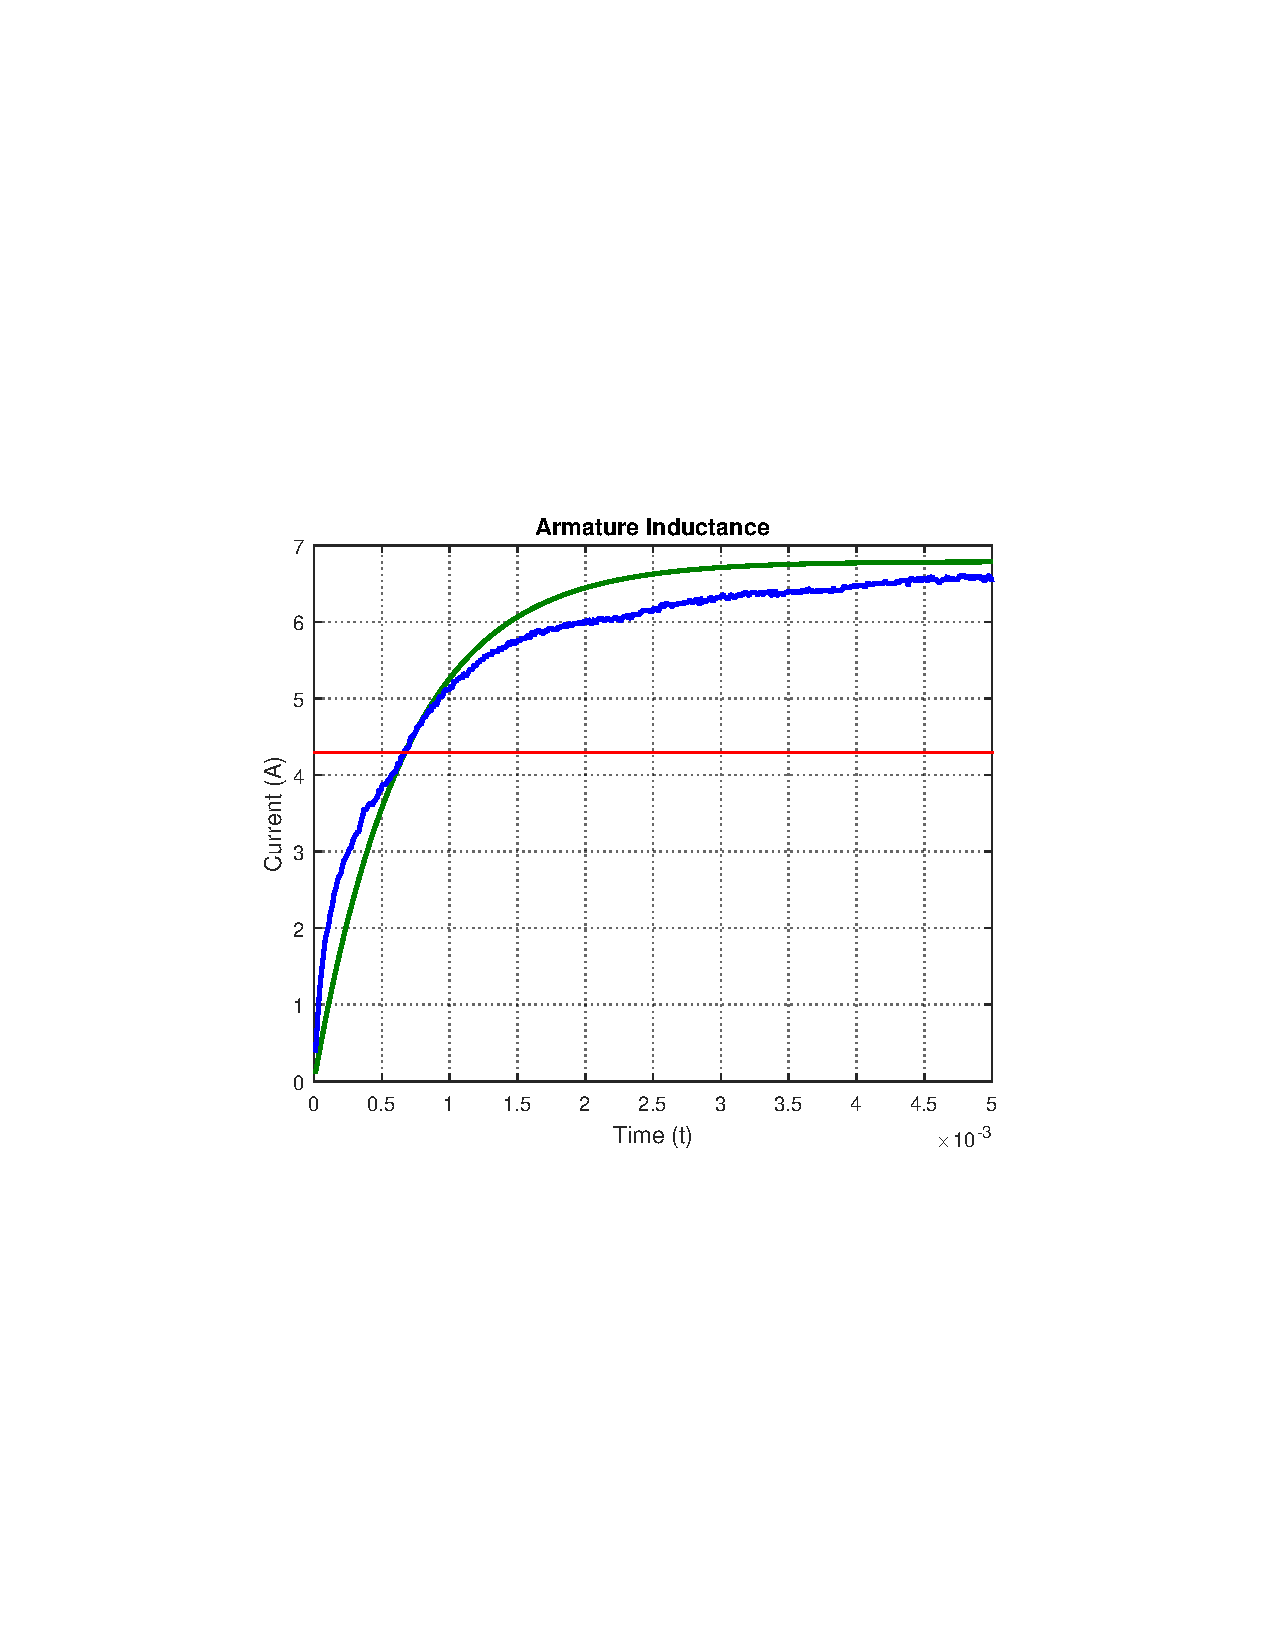
\includegraphics[width=\textwidth]{figures/armatureInductance.pdf}
  }
	\caption{A plot of a current step response of the motor, where the blue line is data, the green line is the ideal step response and the red line is the time constant}
	\label{armatureInductance}
\end{figure}

The armature inductance, \si{L_a}, is calculated from the time constant given by:
\begin{flalign}
  \eq{\tau} {\frac{L_a}{R_a}}\unit{s}\nonumber
\end{flalign}
\hspace{6mm} Where:\\
\begin{tabular}{p{1cm}ll}
  & \si{\tau} & is the time constant \unit{s}       \\
  & \si{L_a}  & is the armature inductance \unit{H} \\
  & \si{R_a}  & is the armature resistance \unit{\Omega} \\
\end{tabular}

\si{R_a} is know from the previous test, \textit{Armature Resistance}, where it was found to \si{0,178 \Omega}. $\tau$ is the time at which the current reaches \si{63,2\%} of the value at steady state. This value of $\tau$ is found by use of \figref{armatureInductance} and located in the data set:
%
\begin{flalign}
  \eq{\tau}{0,67 \cdot 10^{-3}}\unit{s}\nonumber
\end{flalign}
%
From this we get the armature inductance:
%
\begin{flalign}
  \eq{L_a}{\tau \cdot R_a}\unit{H}\nonumber\\
  \eq{L_a} {0,67 \cdot 10^{-3} \cdot 0,178}\unit{H}\nonumber\\
  \eq{L_a}{119,26}\unit{\mu H}\nonumber
\end{flalign}
\pagebreak
\subsection{Tachometer Constant} %\label{put a label here and uncomment}
\textbf{Name: Group 510}\\
\textbf{Date: 30/09 - 2015}

\subsubsection{Purpose}
The purpose of the test is to measure verify that tachometer constant (in V) is 0,030 multiplied by the motor velocity in radians per second.

\subsubsection{Setup}
\begin{figure}[H]
  \centering
	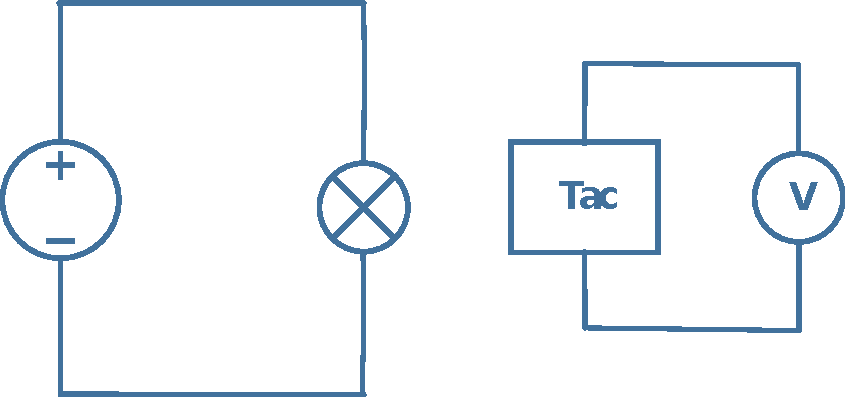
\includegraphics[scale=0.5]{figures/MotorTest3.pdf}
	\caption{Setup Diagram}
	\flushleft
\end{figure}

\subsubsection{List of Equipment}

\begin{table}[H]
\begin{tabular}{|l|l|p{4cm}|}
\hline%--------------------------------------------------------------------------------
  \textbf{Instrument}                    &  \textbf{AAU-no.}  &  \textbf{Type}       \\
\hline%--------------------------------------------------------------------------------
  Power Supply ($0 - 32$ V) ($0 - 10$ A) &  77076             &  Ea - ps 7032 - 100  \\
\hline%--------------------------------------------------------------------------------
  Multimeter                             &  60764             &  Fluke 189 True RMS  \\
\hline%--------------------------------------------------------------------------------
  Optical tachometer                     &  08246             &  Shimpo DT-205       \\
\hline%--------------------------------------------------------------------------------
\end{tabular}
\end{table}

\subsubsection{Procedure}

\begin{enumerate}
  \item Adjust voltage of power supply till the multimeter reaches $6$ V over the tachometer.
  \item Measure the RPM with the Optical tachometer.
\end{enumerate}

\subsubsection{Results}
The tachometer measured 1933 RPM at 6 V, which is used to verify a tachometer constant of \SI{0,03}:
%
\begin{flalign}
 \frac{1933}{60} \cdot 2 \cdot \pi \cdot \num{0,03} &= \num{6,07} \approx 6 \unit{V}
  \label{eqTachometerConstant}
\end{flalign}
\subsection{Generator Constant} %\label{put a label here and uncomment}
\textbf{Name: Group 510}\\
\textbf{Date: 30/09 - 2015}

\subsubsection{Purpose}
The purpose of the test is to find the generator constant $K_e$ by measuring the motor voltages, currents and velocities, in several steady states.

\subsubsection{Setup}
\begin{figure}[H]
  \centering
	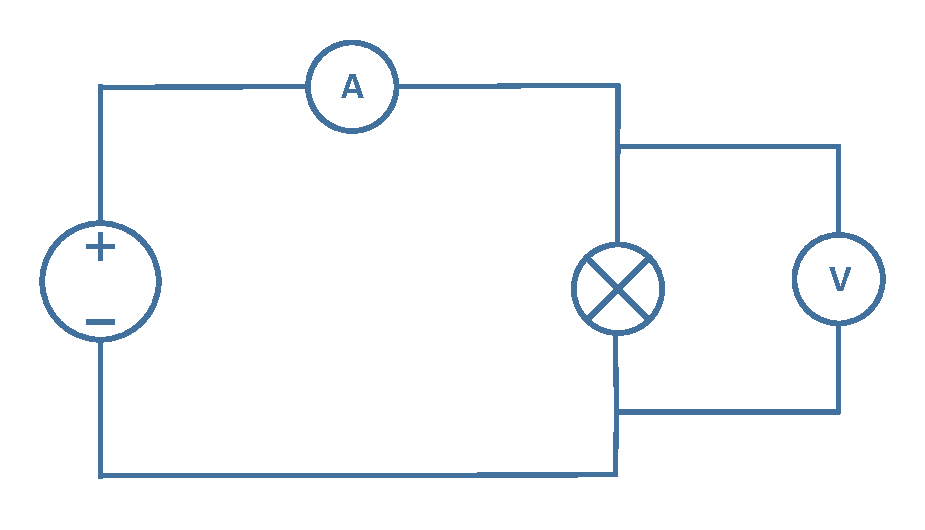
\includegraphics[scale=0.5]{figures/MotorTest4.pdf}
	\caption{Use-Case Diagram}
\end{figure}

\subsubsection{List of Equipment}

\begin{table}[H]
\begin{tabular}{|l|l|p{4cm}|}
\hline%------------------------------------------------------------------------------------
  \textbf{Instrument}                        &  \textbf{AAU-no.}  &  \textbf{Type}       \\
\hline%------------------------------------------------------------------------------------
  Multimeter 1                               &  60764             &  Fluke 189 True RMS  \\
\hline%------------------------------------------------------------------------------------
  Multimeter 2                   		         &  60769             &  Fluke 189 True RMS  \\
\hline%------------------------------------------------------------------------------------
  Power Supply ($0 - 32$ V) ($0 - 10$ A)     &  77076             &  Ea - ps 7032 - 100  \\
\hline%------------------------------------------------------------------------------------
  Optical tachometer                         &  08246             &  Shimpo DT-205       \\
\hline%------------------------------------------------------------------------------------
\end{tabular}
\end{table}

\subsubsection{Procedure}

\begin{enumerate}
  \item Turn on the two multimeters and put them in ampere and voltage mode respectively.
  \item Apply $1$ V by use of the voltage mode multimeter
  \item Read out the current value from the ampere mode multimeter
  \item Read out RPM of the motor using the optical tachometer.
  \item Repeat the past $3$ steps up to $7$ V in $1$ V increments.
\end{enumerate}

\subsubsection{Results}

\begin{table}[H]
\begin{tabular}{|l|l|l|l|}
\hline%----------------------------------------------------------------
  \textbf{Input (V)}  & \textbf{Output (A)} & \textbf{Output (RPM)} & \textbf{Generator constant} \\
\hline%----------------------------------------------------------------
  $1$                 &            $1.7$  &  $3684$ & $0.00181$                 \\
\hline%----------------------------------------------------------------
  $2$                 &            $2.2$  &  $8063$ & $0.00191$                 \\
\hline%----------------------------------------------------------------
  $3$                 &            $2.6$  &  $12021$ & $0.00202$                \\
\hline%----------------------------------------------------------------
  $4$                 &            $3.3$  &  $16746$ & $0.00195$                \\
\hline%----------------------------------------------------------------
  $5$                 &            $4.1$  &  $21966$ & $0.00186$                \\
\hline%----------------------------------------------------------------
  $6$                 &            $4.8$  &  $26420$ & $0.00186$                \\
\hline%----------------------------------------------------------------
  $7$                 &            $5.6$  &  $31447$ & $0.00182$                \\
\hline%----------------------------------------------------------------
\end{tabular}
\end{table}

The equation for the generator constant is $K_e = \frac{U_a - R_a I_a}{\omega}$. The generator constants for each measurement is not equal, but with a small margin in difference. The average generator constant is $0.00189$.
\pagebreak
\subsection{Motor Constant} %\label{put a label here and uncomment}
\textbf{Name: Group 510}\\
\textbf{Date: 30/09 - 2015}

\subsubsection{Purpose}
The purpose of this of this test is to measure the motor constant \si{K_t}.

\subsubsection{Setup}
\begin{figure}[H]
  \centering
	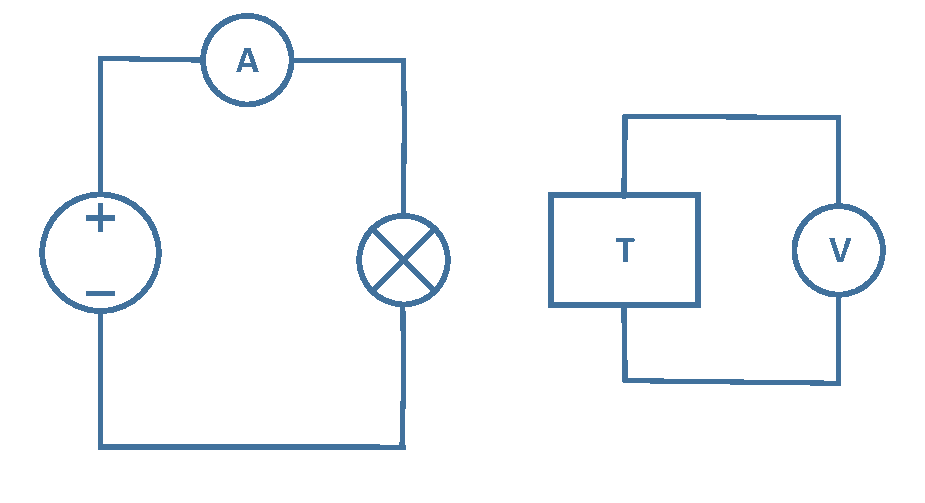
\includegraphics[scale=0.5]{figures/MotorTest5.pdf}
	\caption{Setup diagram}
\end{figure}

\subsubsection{List of Equipment}

\begin{table}[H]
\begin{tabular}{|l|l|p{4cm}|}
\hline%------------------------------------------------------------------------------------
  \textbf{Instrument}                        &  \textbf{AAU-no.}  &  \textbf{Type}       \\
\hline%------------------------------------------------------------------------------------
  Multimeter 1                               &  60764             &  Fluke 189 True RMS  \\
\hline%------------------------------------------------------------------------------------
  Multimeter 2                   		         &  60769             &  Fluke 189 True RMS  \\
\hline%------------------------------------------------------------------------------------
  Power Supply ($0 - 32$ V) ($0 - 10$ A)     &  77076             &  Ea - ps 7032 - 100  \\
\hline%------------------------------------------------------------------------------------
  Torque sensor                              &  08772             &  Icom                \\
\hline%------------------------------------------------------------------------------------
\end{tabular}
\end{table}

\subsubsection{Procedure}

\begin{enumerate}
  \item Connect the motor shaft to the torque sensor.
  \item Turn on the two multimeter in current and voltage mode respectively.
  \item Start by setting the power supply at 1 A current limiting.
  \item Turn on the supply and note the voltage across the torque sensor.
  \item Repeat the previous two steps up to 10 A with 1 A increments.
\end{enumerate}

\subsubsection{Results}

\begin{table}[H]
\begin{tabular}{|l|l|l|}
\hline%-----------------------------------------
  \textbf{Input (A)}  & \textbf{Output (V)}  \\
\hline%-----------------------------------------
  $1$                 &            0,107    \\
\hline%-----------------------------------------
  $2$                 &            0,113    \\
\hline%-----------------------------------------
  $3$                 &            0,118    \\
\hline%-----------------------------------------
  $4$                 &            0,122    \\
\hline%-----------------------------------------
  $5$                 &            0,131    \\
\hline%-----------------------------------------
  $6$                 &            0,142    \\
\hline%-----------------------------------------
  $7$                 &            0,149    \\
\hline%-----------------------------------------
  $8$                 &            0,158    \\
\hline%-----------------------------------------
  $9$                 &            0,169    \\
\hline%-----------------------------------------
  $10$                &            0,180    \\
\hline%-----------------------------------------
\end{tabular}
\end{table}

\begin{figure}[H]
  \centering
 	%Trim margins @:   left        bottom       right       top
 	\adjustbox{ trim = {.15\width} {.30\height} {.15\width} {.30\height}, clip }
  {
    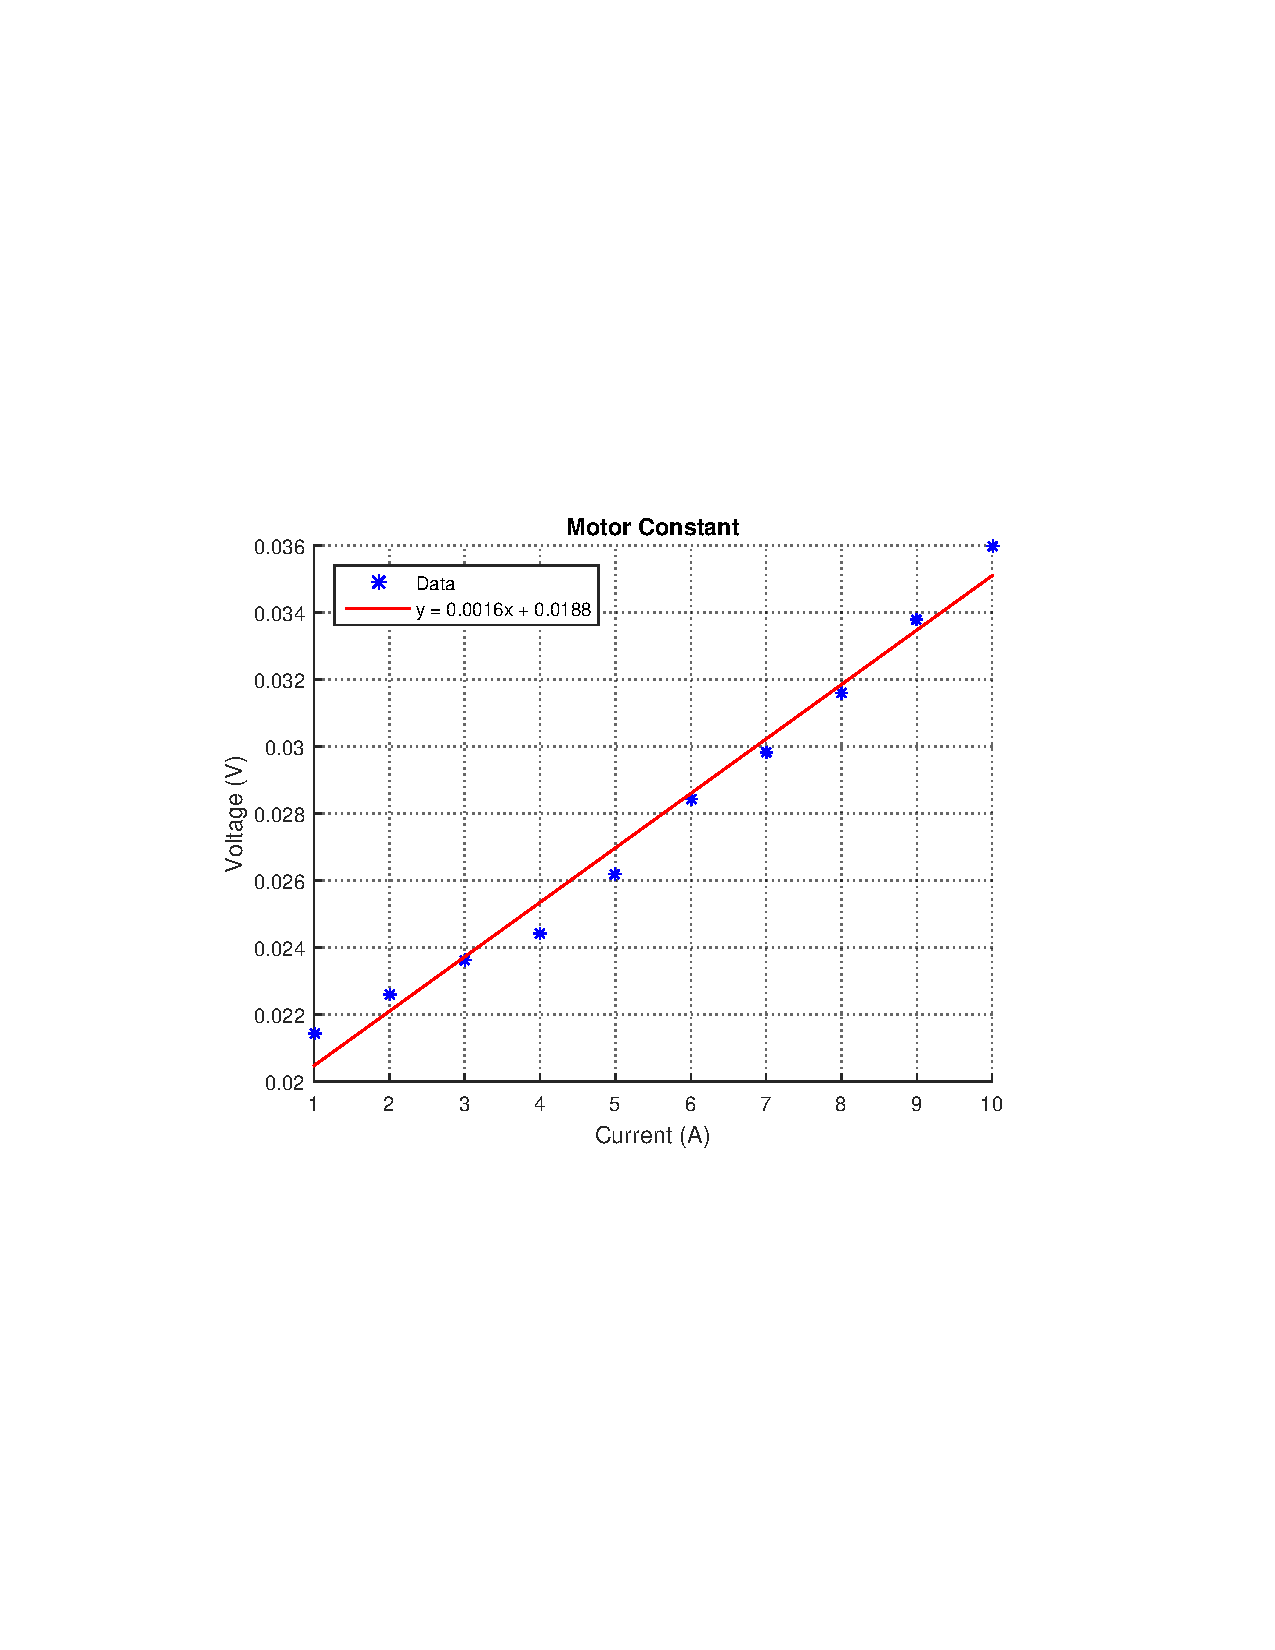
\includegraphics[width=\textwidth]{figures/motorConstant.pdf}
  }
	\caption{A plot of the torque at different currents, where the blue dots is the measurements and the red line is the least square line.}
	\label{motorConstant}
\end{figure}

The voltages measure are scaled by factor of 0,2 since the torque sensor outputs 5 V per \si{100N\cdot cm} giving a torque of 0,2 \si{N\cdot m/V} \cite{MWAW81P}.
After scaling the voltages to torques it is plotted and a lest square line is added as seen on \figref{motorConstant}. The relation between the current and torque is described as follows:

\begin{flalign}
  \eq{\tau}{K_t \cdot I_a}\unit{N\cdot m}\nonumber\\
  \eq{K_t} {\frac{\tau}{I_a}}\unit{N\cdot m \cdot A^{-1}}\nonumber
\end{flalign}
\hspace{6mm} Where:\\
\begin{tabular}{p{1cm}lll}
  & \si{\tau}   & is the torque                        &\unitWh{N\cdot m}\\
  & \si{I_a}    & is the current supplied to the motor &\unitWh{A}\\
  & \si{K_t}    & is the motor constant                &\unitWh{N\cdot m \cdot A^{-1}}
\end{tabular}

The value of \si{K_t} is then extracted directly as the slope of the least square regression:
\begin{flalign}
  \eq{K_t}{\num{0,0016}} \ \si{N\cdot m \cdot A^{-1}}&\nonumber
\end{flalign}
\pagebreak
\subsection{Motor Friction} %\label{put a label here and uncomment}
\textbf{Name: Group 510}\\
\textbf{Date: 30/09 - 2015}

\subsubsection{Purpose}
The purpose of the test is to find the motor friction, B, by measuring the motor current and the corresponding velocities, in several steady states.

\textbf{The data from the test \textit{Generator Constant} is reused, and so the equipment and setup is the same.}

\subsubsection{Results}
%
\begin{table}[H]
\begin{tabular}{|l|l|l| l|l|}
\cline{1-2}\cline{4-5}%-------------------------             -------------------------------------------------
  \textbf{Input (A)}   & \textbf{Output (RPM)} &\phantom{hey}& \textbf{Input (A)}   & \textbf{Output (RPM)} \\
\cline{1-2}\cline{4-5}%-------------------------             -------------------------------------------------
  1,7                &             $3684$    &             & 4,1                & $21966$               \\
\cline{1-2}\cline{4-5}%-------------------------             -------------------------------------------------
  2,2                &             $8063$    &             & 4,8                & $26420$               \\
\cline{1-2}\cline{4-5}%-------------------------             -------------------------------------------------
  2,6                &             $12021$   &             & 5,6                & $31447$               \\
\cline{1-2}\cline{4-5}%-------------------------             -------------------------------------------------
  3,3                &             $16746$  \\
\cline{1-2}%------------------------------------
\end{tabular}
\end{table}
%
\begin{figure}[H]
  \centering
 	%Trim margins @:   left        bottom       right       top
 	\adjustbox{ trim = {.15\width} {.30\height} {.15\width} {.30\height}, clip }
  {
    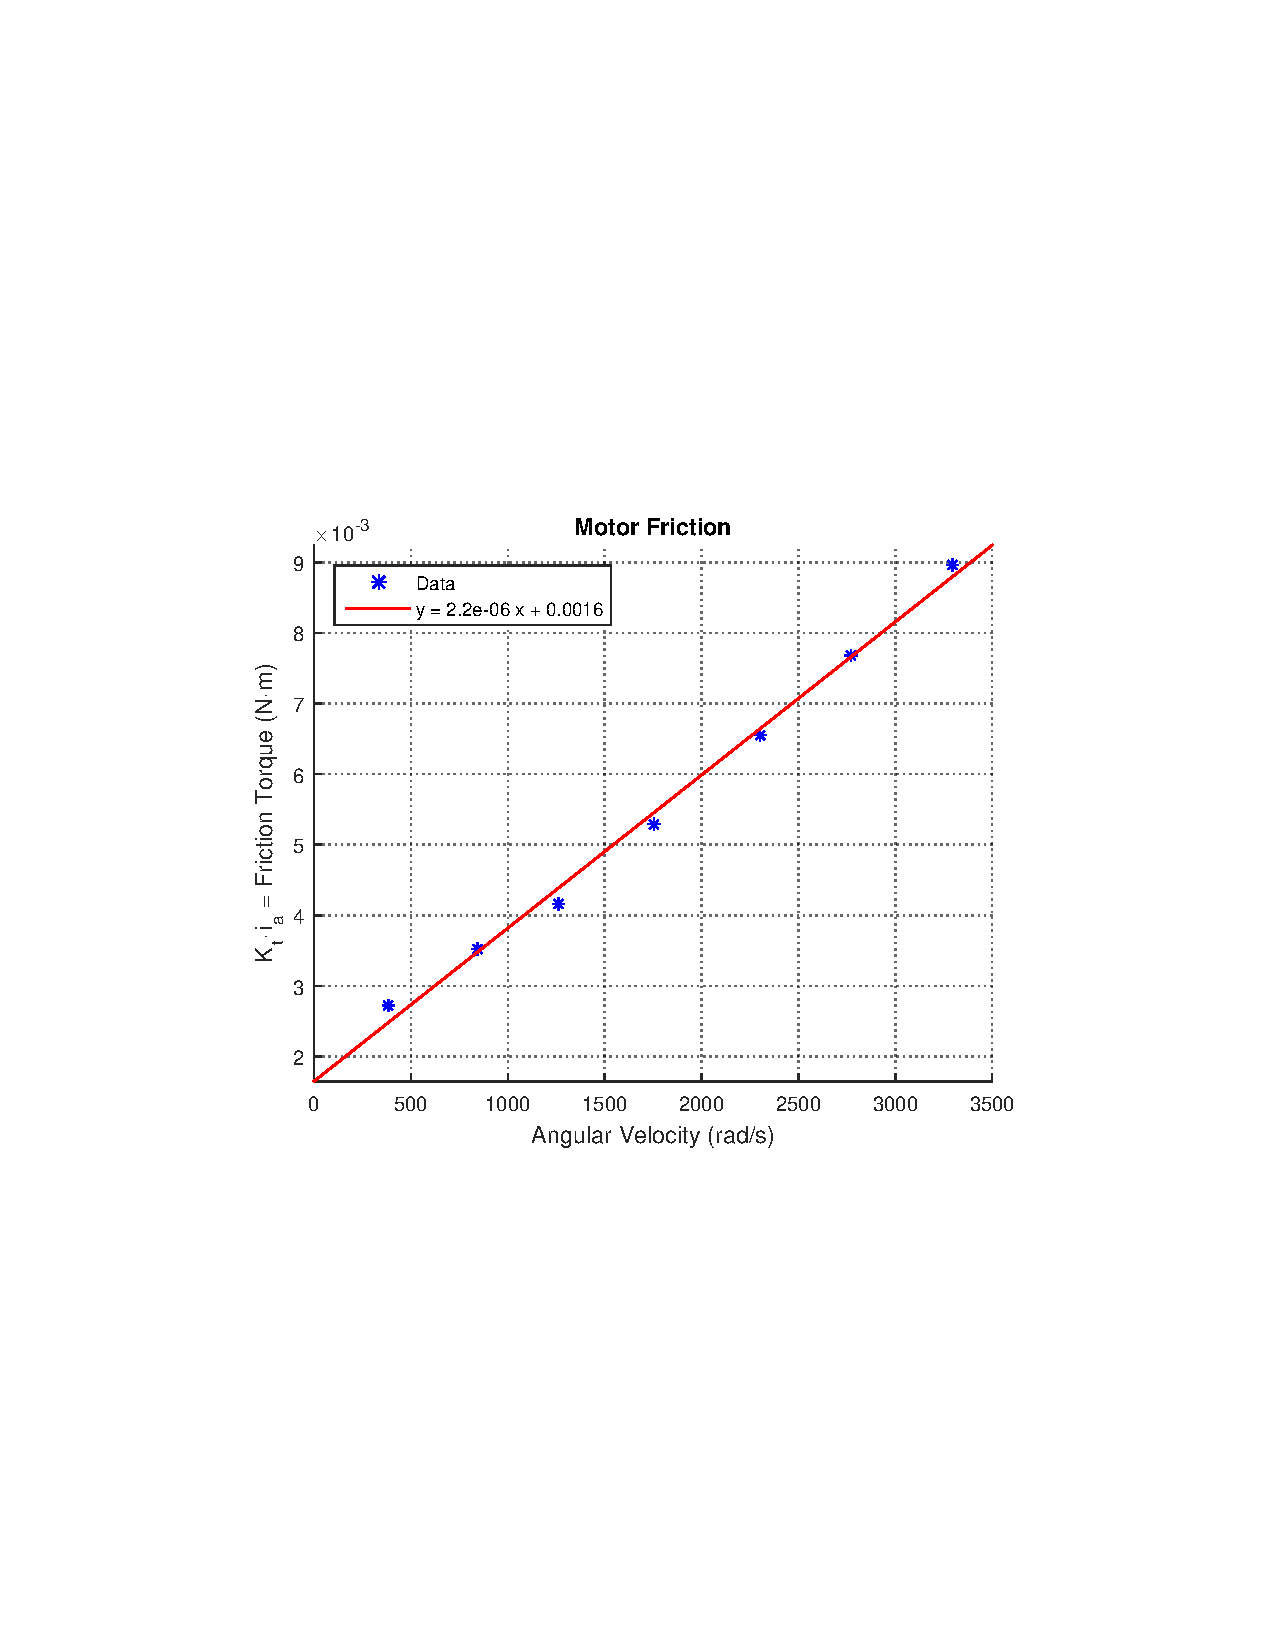
\includegraphics[width=\textwidth]{figures/motorFriction.pdf}
  }
	\caption{Plot of test results}
	\label{motorFriction}
\end{figure}

The following equation is applied to obtain the motor friction:

\begin{align}
  \eq{B}{\frac{K_t \cdot I_a}{\omega}} \unit{N\cdot m \cdot s}\nonumber
\end{align}

\hspace{6mm} Where:\\
\begin{tabular}{p{1cm}ll}
  & \si{K_t}   & is the motor constant \unit{N\cdot m \cdot A^{-1}}  \\
  & \si{I_a}   & is the armature current \unit{A}                    \\
  & \si{B}     & is the motor friction \unit{N\cdot m \cdot s}       \\
  & \si{\omega}& is the motor angular velocity \unit{s ^{-1}}                \\
\end{tabular}

This relationship is plotted in \figref{motorFriction} and a least square line is added. The friction, B, is found as the slope and the Coulomb friction (stiction), \si{\tau_c}, is the interception between the least square line and the y-axis.

\begin{align}
  \eq{B}{\num{2,2}\cdot 10^{-6}} \unit{N\cdot m}\nonumber\\
  \eq{\tau_c}{\num{0.0016}} \unit{N\cdot m}\nonumber
\end{align}
\pagebreak
\subsubsection{Moment of Inertia} %\label{put a label here and uncomment}
\textbf{Name: Group 510}\\
\textbf{Date: 30/09 - 2015}

\subsubsection{Purpose}
The purpose of this test is to find the moment of inertia $I$, by measuring the motor velocity as a function of time.

\subsubsection{Setup}
Test setup

\subsubsection{List of Equipment}

\begin{table}[H]
\begin{tabular}{|l|l|p{4cm}|}
\hline%------------------------------------------------------------------------------------
  \textbf{Instrument}                        &  \textbf{AAU-no.}  &  \textbf{Type}       \\
\hline%------------------------------------------------------------------------------------
  Oscilloscope                               &  64672             &  Agilent DSO6034A    \\
\hline%------------------------------------------------------------------------------------
  Power Supply ($0 - 32$ V) ($0 - 10$ A)     &  77076             &  Ea - ps 7032 - 100  \\
\hline%------------------------------------------------------------------------------------
  Optical tachometer                         &  77087             &  Compact             \\
\hline%------------------------------------------------------------------------------------
\end{tabular}
\end{table}

\subsubsection{Procedure}

\begin{enumerate}
  \item Turn on the oscilloscope.
  \item On the oscilloscope press the "mode"-key choose the "normal"-option, set the trigger to "falling edge".
  \item To prevent false triggering on the oscilloscope set the trigger value to %\fxnote{input value from extracted data} mV with the turn-key.
  \item Turn on the power supply at 7 volt.
  \item Press "single"-key on oscilloscope and cut the power of the motor.
  \item Insert a USB-pin in the oscilloscope and press the save key to extract the data.
\end{enumerate}

\subsubsection{Results}

\begin{figure}[H]
	\centering
	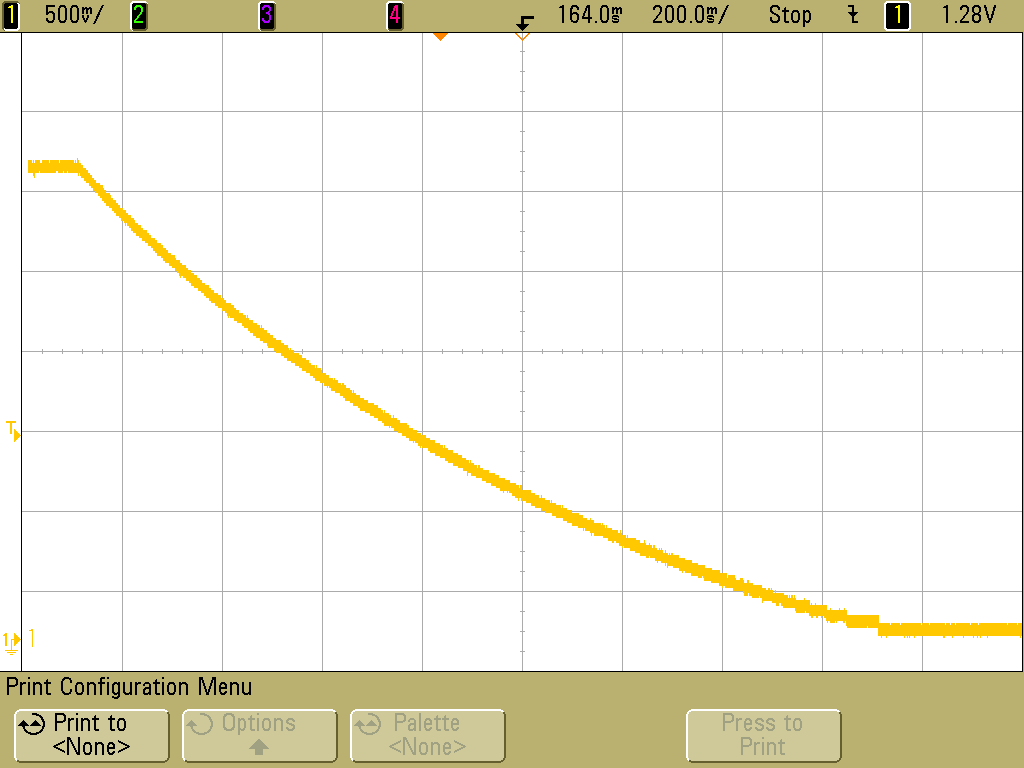
\includegraphics[scale=.4]{figures/Exercise7}
	\caption{Plot of test results}
\end{figure}
\pagebreak
\subsection{Time Constant and Gain} %\label{put a label here and uncomment}
\textbf{Name: Group 510}\\
\textbf{Date: 30/09 - 2015}

\subsubsection{Purpose}
The purpose of this test is to find the motors time constant $\tau$ and gain. This is done by measuring the motors step response.

\subsubsection{Setup}
\begin{figure}[H]
  \centering
	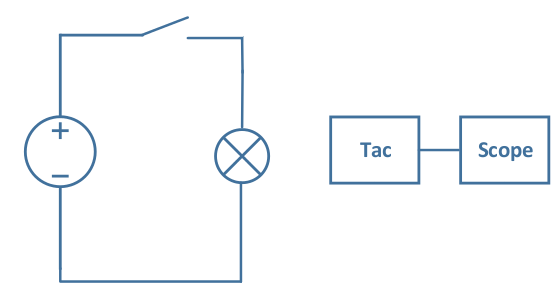
\includegraphics[scale=0.5]{figures/MotorTest8.png}
	\caption{Setup diagram}
\end{figure}

\subsubsection{List of Equipment}

\begin{table}[H]
\begin{tabular}{|l|l|p{4cm}|}
\hline%------------------------------------------------------------------------------------
  \textbf{Instrument}                        &  \textbf{AAU-no.}  &  \textbf{Type}       \\
\hline%------------------------------------------------------------------------------------
  Oscilloscope                               &  64672             &  Agilent DSO6034A    \\
\hline%------------------------------------------------------------------------------------
  Power Supply ($0 - 32$ V) ($0 - 10$ A)     &  77076             &  Ea - ps 7032 - 100  \\
\hline%------------------------------------------------------------------------------------
  Optical tachometer                         &  77087             &  Compact             \\
\hline%------------------------------------------------------------------------------------
\end{tabular}
\end{table}

\subsubsection{Procedure}

\begin{enumerate}
  \item Turn on the oscilloscope, and connect one channel to the power supply, and another to the tachometer.
  \item On the oscilloscope press the "trigger mode"-key choose the "normal"-option, set the trigger to "rising-edge", and the trigger source to the channel connected to the power supply.
  \item To prevent false triggering on the oscilloscope set the trigger value to \num{4,50}V with the turn-key.
  \item Press "single"-key on oscilloscope.
  \item Turn on the power supply at 5 volt.
  \item Insert a USB-flash drive in the oscilloscope and press the save key to extract the data.
\end{enumerate}

\subsubsection{Results}

\begin{figure}[H]
  \centering
  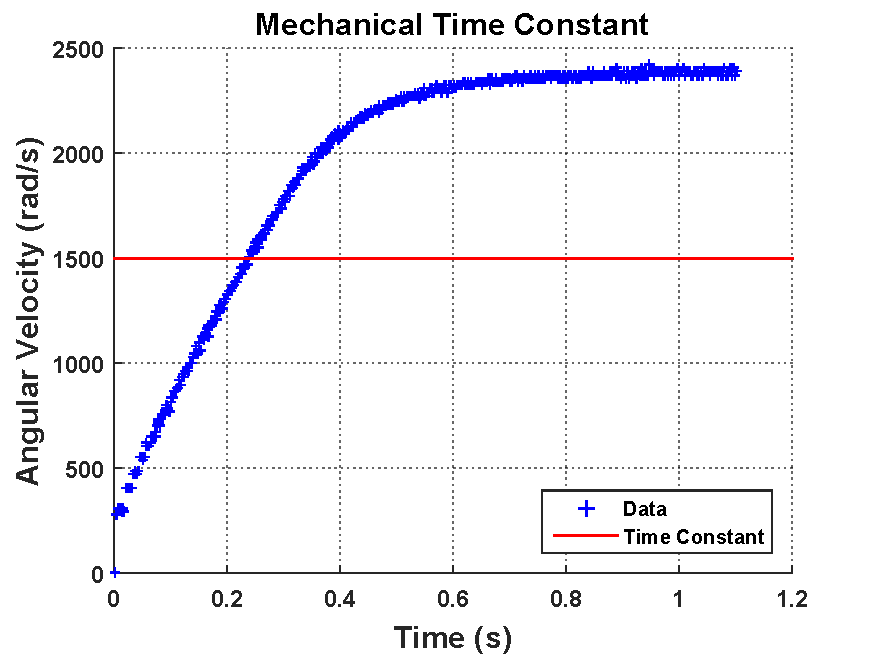
\includegraphics[width=.8\textwidth]{figures/mechanicalTimeConstant.pdf}
	\caption{A plot of the step response illustrating the angular velocity over time. The blue dots is the measurements and the red line indicates the mechanical time constant.}
	\label{mechanicalTimeConstant}
\end{figure}

The graph in \figref{mechanicalTimeConstant} shows the angular velocity of the motor over time. The read line shows the time constant at \si{\num{63.2} \%} of max angular velocity. In the data the mechanical time constant is found to be:
%
\begin{flalign}
  \eq{\tau_{mec}}{0,238} \tx{ s}&&\nonumber
\end{flalign}

\begin{figure}[H]
  \centering
 	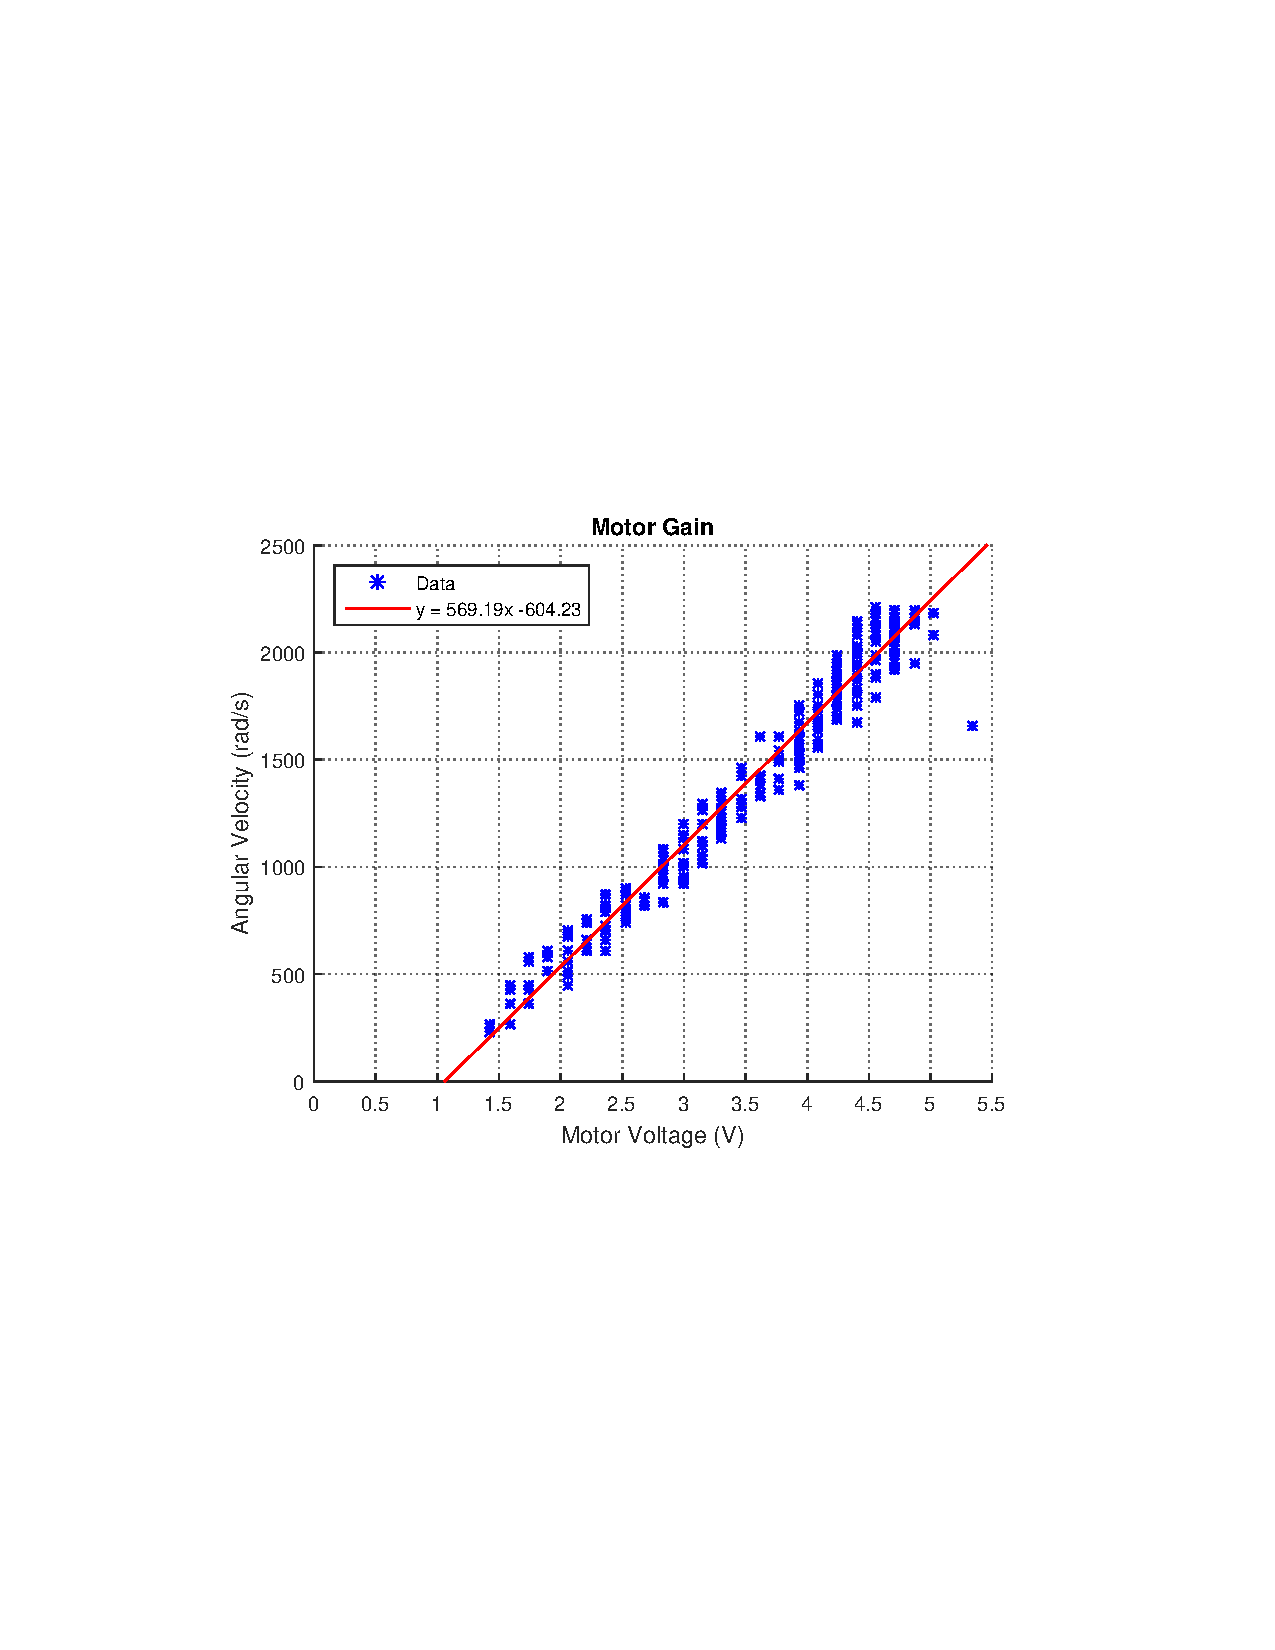
\includegraphics[width=.8\textwidth]{figures/motorGain.pdf}
  \caption{A plot of the motor's step response, where the input is motor voltage and the output is the angular velocity. The blue dots indicates the measurements and the red line is the tendency line.}
	\label{motorGain}
\end{figure}

The graph in \figref{motorGain} shows motor voltage in relation to the angular velocity, which reveals the gain, \si{K} of the system, as the slope of the least square regression line:
%
\begin{flalign}
  \eq{K}{\num{569.19}} \unit{\cdot}\nonumber
\end{flalign}

\pagebreak
\section{Inertia Test}
\nopagebreak
%\subsection{} %\label{put a label here and uncomment}
\textbf{Name: Group 510}\\
\textbf{Date: 30/09 - 2015 to change}

\subsubsection{Purpose}
The purpose of the test is to measure inertia of the loaded vehicle.

\subsubsection{Setup}
\begin{figure}[H]
	\centering
	%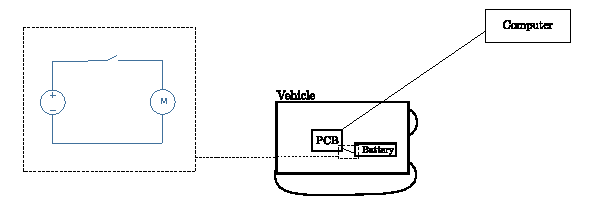
\includegraphics[scale=0.5]{figures/inertiaTestSetupDiagram.pdf}
	\caption{Setup diagram}
	\label{inertiaTestSetupDiagram}
\end{figure}

\subsubsection{List of Equipment}


\subsubsection{Procedure}

\begin{enumerate}
  \item Connect the vehicle to the computer via the arduino card, and disconnect the battery.
  \item Launch the arduino program.
  \item Plug in the battery so the vehicle runs.
  \item After a few seconds of running, take off the two wires connected to the PCB to stop powering the vehicle.
  \item Wait until the vehicle stops to end measuring the speed of it.
  \item Plot the speed of the vehicle.
\end{enumerate}

\subsubsection{Results}

\begin{figure}[H]
  \centering
  %\includegraphics[scale=0,5]{figures/InertiaTestPlot.pdf}
  \caption{Plot of the inertia measured speed of the vehicle at constant speed and unpowered at the end.}
  \label{intertiaTestPlot}
\end{figure}

During these measurements the motor is at constant speed until the end when it is unpluged.

%---------- Appendix C ---------------------------------------- Friction Test
\pagebreak
\subsection{Friction test} %\label{put a label here and uncomment}
\textbf{Name: Group 510}\\
\textbf{Date: 28/10 - 2015}

\subsubsection{Purpose}
The purpose of the test is to find the total friction, $B$, of the vehicle.

\subsubsection{Setup}
\begin{figure}[H]
  \centering
	\includegraphics[scale=0.5]{figures/FrictionTest.pdf}
	\caption{A diagram of the test setup}
\end{figure}

\subsubsection{List of Equipment}

\begin{table}[H]
\begin{tabular}{|l|l|p{4cm}|}
\hline%------------------------------------------------------------------------------------
  \textbf{Instrument}                        &  \textbf{AAU-no.}  &  \textbf{Type}       \\
\hline%------------------------------------------------------------------------------------
  Multimeter                               &  60764             &  fluke 189 true RMS    \\
\hline%------------------------------------------------------------------------------------
  Power Supply ($0 - 32$ V) ($0 - 10$ A)     &  77075             &  Ea - ps 7032 - 100  \\
\hline%------------------------------------------------------------------------------------
  Treadmill                         &  75483             &  Rodby            \\
\hline%------------------------------------------------------------------------------------
\end{tabular}
\end{table}

\subsubsection{Procedure}

\begin{enumerate}
  \item Connect the power supply's power channel to the motor and the ground channel to the multimeter.
  \item Place the vehicle in the middle of the treadmill.
  \item Set the power channel to under $4$ amperes, the vehicle is not running, but ready to run when the power supply is set above $4$ amperes later. 
  \item Activated the treadmill to run at the required speed, and at the same time correct the power supply so the vehicle receives more than $4$ amperes and thereby making it move.
  \item Correct the speed of the vehicle with the power supply until the vehicle has the same velocity as the treadmill.
  \item Read the current on the multimeter.
  \item Repeat the process with different velocities.
\end{enumerate}

\subsubsection{Results}
The Raw data extracted from the measurements is the vehicle's velocity in $[km \cdot hour^{-1}]$ and the current needed for achieving the specific velocity. The velocity is calculated from $[km \cdot hour^{-1}]$ to a linear velocity $[m \cdot s^{-1}]$:

\begin{align}
\eq{V}{\frac{V_m \cdot 10^{3}}{3600}} \unit{m \cdot s^{-1}}
\end{align}
\hspace{6mm} Where:\\
\begin{tabular}{p{1cm}ll}
& $V_m$ & is measured velocity of the vehicle [$km \cdot hour^{-1}$] \\
& V & is the vehicle's linear velocity [$m \cdot s^{-1}$] \\
\end{tabular}

By using linear velocity $[m \cdot s^{-1}]$, the motors angular velocity $[rad \cdot s^{-1}]$ can be calculated:

\begin{align}
\eq{\omega_m}{\frac{V \cdot N}{r_t}} \unit{rad \cdot s^{-1}}
\end{align}
\hspace{6mm} Where:\\
\begin{tabular}{p{1cm}ll}
& \si{\omega_m} & is the motor's angular velocity [$\frac{rad}{s}$] \\
& N & is the gear ratio of the vehicle  [$\cdot$]\\
& $r_t$ & is the radius of the two wheels driving the belts [$m$] \\
\end{tabular}

The motor's torque and angular velocity is plotted: 

\begin{figure}[H]
  \centering
	\includegraphics[scale=1]{figures/FrictionTestPlot.png}
	\caption{A plot of the motor's torque over the motor's angular velocity. The blue dots indicates the measurements and the red line is the tendency line.}
	\label{TotalFriction}
\end{figure}

The red line in \figref{TotalFriction} is the tendency line, the slope indicates the friction and the offset is the stiction of the system. The total friction of the system is therefore:

\begin{align}
\eq{B_{tot}}{4.7*10^{-6}} \unit{N \cdot m \cdot rad^{-1} \cdot s}
\end{align}
%\pagebreak
\section{Steering test} %\label{put a label here and uncomment}
\textbf{Name: Group 510}\\
\textbf{Date: 28/10 - 2015}

\subsection{Purpose}
The purpose of the test is to find the needed order of the steering model.

\subsection{Theory}


What is the input and output of the test?

cirkel figure

cirkel figure description (avoiding measuring angle to improve accdapowjda.)

(The hall sensor is not used for putting points around the arc, since just taking manual point will be faster, furthermore we will not use it to get the angle, because it will be to difficult to get an exact angle)

equations from the cirkel:

radius

angular velocity

\subsection{Setup}
\begin{figure}[H]
  \centering
	\includegraphics[scale=0.5]{figures/FrictionTest.pdf}
	\caption{A diagram of the test setup}
\end{figure}

\subsection{List of Equipment}

\begin{table}[H]
\begin{tabular}{|l|l|p{4cm}|}
\hline%------------------------------------------------------------------------------------
  \textbf{Instrument}                       &  \textbf{AAU-no.}  &  \textbf{Type}         \\
\hline%------------------------------------------------------------------------------------
  Multimeter                                &  60764             &  Fluke 189 true RMS    \\
\hline%------------------------------------------------------------------------------------
  Power Supply ($0 - 32$ V) ($0 - 10$ A)    &  77075             &  Ea - ps 7032 - 100    \\
\hline%------------------------------------------------------------------------------------
  Treadmill                                 &  75483             &  Rodby                 \\
\hline%------------------------------------------------------------------------------------
\end{tabular}
\end{table}

\subsection{Procedure}

\begin{enumerate}
  \item C
  \item P
  \item S
  \item A
  \item C
  \item R
  \item R
\end{enumerate}

\subsection{Results}




%%% Bibliography %%%
\printbibliography

%%% To Do List %%%
\listoftodos

\end{document}